\part{新帝国主义理论}

\chapter{资本主义与不发达}

\section{引言}

第二篇集中分析了发达资本主义的功能及其转化。每种理论都谋求对“\textbf{长期繁
  荣}”提供一种解释,理解使它最终受到削弱的矛盾,因此而说明西方工人阶级的被动状态,
也为将来的激进化运动寻找根据。在所有的情况下,落后地区的经济结构及其与发达国家经
济结构的关系,几乎都不在考虑之列。只有巴兰和斯威齐认为它们比较重要,但即使如此,
它们在《垄断资本》中的重要性也只是第二位的。资本主义中心地带稳定和变化的力量,在
根本上被认为是通过主要资本主义国家经济的再生产和增长来起作用的。

但是,第二次世界大战之后,\textbf{其他地区的落后变得越来越明显}。那时,发达国家平
均的单位资本收入比不发达地区高4倍,18世纪中期这两者大约是相等的,再早200年,很多
非欧洲国家比欧洲还要富。此外,作为一种政治力量,马克思主义主要是在不发达地区获得
了发展,而且马克思主义者自然觉得有必要把自己与落后连在一起。这一点本身并不新鲜。
正如本书第一卷所证明的,俄国的马克思主义者曾详细思考过这个问题。战后出现的理论的
新奇之处在于,它们认为\textbf{落后是不发达进程的结果},在这一进程中,发达资本主义
经济为了阻碍落后地区的发展而扭曲其经济结构。当然,马克思主义者总是认为帝国主义剥
削有助于主要资本主义国家的经济增长。但在20年代之前,他们还认为西方的冲击在全球范
围内刺激了经济的发展。马克思、恩格斯、考茨基、卢森堡、希法亭以及列宁、布哈林、托
洛茨基都普遍相信,帝国主义促进了资本主义经济的发展。

当然,这一问题从来不是这些马克思主义者著作论述的主题,这些马克思主义者是高度的欧
洲中心主义者。甚至他们对“帝国主义”这个词的使用也反映了这一点。例如,列宁把帝国
主义用作资本主义垄断阶段的同义词,而希法亭和卢森堡则把帝国主义与争夺“经济版
图”等同起来。发达国家对不发达国家的控制和剥削,在战后已经具有主要的涵义,但
在1917年之前,甚至在两次世界大战期间,它的确没被普遍提及。只有考茨基和卢森堡比较
接近这个涵义,他们强烈地抵制这种新用法与政治的联系,在这种新用法中,人们常常会认
为“阶级斗争”在现在就意味着剥削和被剥削民族之间的斗争(见以下第3节)。

对已有的帝国主义理论进行修正的责任落到保罗·巴兰身上。在50年代初,他就系统地阐述了
关于不发达分析的大部分主要的经济学命题。这些思想的先兆,甚至能够在权威的,
如1928年共产国际的纲要这样的文件中看到(见以下第11章)。两次世界大战期间,斯大林、
托洛茨基和其他俄国马克思主义者的偶然陈述中,也有巴兰著作中的观点。在列宁关于帝国
主义已不再是进步力量的论述中,也明显地可见这种新理论的基础。由于他严重依赖希法亭,
又与布哈林的观点很接近,所以在希法亭和布哈林的著作中也可见新理论的基础(见本书第一
卷第13章)。1920年之后,第三国际提高了殖民地国家反帝斗争的重要性,这无疑也为这种理
论的重新表达提供了有益的推动力。不过,单单是巴兰的著作,就已对传统马克思主义关于
落后国家资本主义经济发展问题作出了明显的突破。\textbf{一个全面的不发达经济理论第
  一次得到了系统阐述,它解释了为什么如果没有社会主义革命的介入,发达资本主义中心
  地带之外的发展就不可能。}巴兰的观点后来虽然被安德烈·冈德·弗兰克、伊曼纽尔·沃勒
斯坦和“依附理论者”加以扩展,但他们对它改进很少(见以下第3节和第4节)。因而,巴兰
可以在现代马克思主义帝国主义理论中占据与希法亭在本世纪初马克思主义帝国主义理论中
相类似的地位。他提供了最重要的概念和主要的思想,并为其他理论家进行新的思考留下了
足够的空间。

对巴兰主要的影响大概来自保罗·斯威齐。他俩之间持久的友谊开始于1939年,而斯威
齐1942年出版的《资本主义发展理论》已简略地暗示了10年后巴兰的观点。但斯威齐日益转
向一种在巴兰的著作中没得到清楚表达的“\textbf{交换的看法}”(参见以下第11章第1节)。
劳尔·普雷维什和其他激进的发展经济学家,可能也提供了一些为巴兰所使用的观点,包括成
为新帝国主义理论标志的“中心”、“外围”等术语。\textbf{但巴兰强调的既不是(他们所
  声称的)阻碍了落后地区经济发展的结构刚性,也不是由此得出的想象中的贸易条件的恶化。
  相反,他强调不发达正是资本主义根本性质发生作用的结果。}苏联经济转型提供的对照显
然给巴兰留下了深刻的印象,计划经济在东欧和中国的扩展,也一样给他留下了深刻的印象。
这导致他否定改良主义:不管多么激进,改良资本主义都不如\textbf{中央计划}所具有的潜
力大,中央计划的本质就是要进行社会主义革命。与殖民地独立运动一道,民族解放运动的
急剧高涨,以及苏联对同盟军及贸易伙伴的需要,这种在巴兰的理论中所具有的斯大林主义
色彩,说明他受到莫里斯·多布以及苏维埃代言人热烈欢迎的原因。

\section{保罗·巴兰和《墤长的政治经济学》}

巴兰对不发达理论的第一次简略论述,是在他1952年发表的《落后的政治经济学》一文中,
之前两年这篇论文曾送交美国经济学会。接着,出版于1957年的《增长的政治经济学》对这
一理论作了进一步的阐述,该书的主要思想是他1953年所作的一系列专题讲座的主题。50年
代和60年代,巴兰还写了一些从多个角度探讨不发达问题的论文,其中一些论文结集以《更
长远的观点》为题于1970年(他已去世)出版。同时,他与保罗·斯威齐合著了《垄断资
本》(见以上第6章)。这本书讲的几乎全是发达资本主义经济结构的问题,但考虑到巴兰关于
落后命题的特性,它也构成其不发达理论的必要的组成部分。

巴兰论述帝国主义问题的核心思想,比马克思主义者还要正统。\textbf{经济的增长是剩余
  的大小及对其利用的结果。}把剩余用于生产性投资,经济就会增长。剩余积累得越多,增
长得就越快。\textbf{经济出现停滞,要么是因为剩余不足以用来扩大生产力;要么是剩余虽
  然丰富却被浪费到非生产消费上了。}这样,\textbf{“中心”与“外围”分化的经济
  史}——生产资料的开发被集中到中心地带,外围地区的发展受到阻止——\textbf{就取决于
  世界剩余产品在不同地区的分配,以及它们在这些地区被使用的方式。}

根据巴兰的观点,这种分化始于16世纪,那是西欧国家开始其殖民扩张和原始积累进程的时
期。在国内的剩余不断地被投入国内生产的同时,\textbf{欧洲以外其他国家的剩余也被补
  充进来使用。这种剩余的转移破坏了拉丁美洲、非洲和大部分东南亚国家的经济增长。}巴
兰断言,自发的资本主义发展的种子,在16世纪到处可见(或者至少在亚洲到处可见)。那时,
在全世界都有可能进行资本积累。但结果却被集中到西欧,仅仅因为\textbf{欧洲对其他地
  区的控制阻碍了那里早期的资产阶级革命,并根据帝国主义中心的利益重塑了那里的经
  济。}西欧在现代历史的发端期所拥有的这点小小的、最初的优势,就这样变成了永久的好
处,并产生了累加的分化。

为了支持这一论点,巴兰指出印度工业的发展早于对它的殖民控制,并展示了印度的经济在
后来是怎样为了英国制造商们的利益而被殖民管理扭曲的:已经建立起来的工业被破坏了,
印度经济生产出来的剩余被帝国吮吸。巴兰还拿日本的命运与印度的经历作对比:日本成功
地逃脱了殖民控制,并因此而保存了自己的工业,使之未受损害,完成了自己的资产阶级革
命,把剩余用于本国的生产性投资。\textbf{根据巴兰的观点,一般说来决定一个国家是获
  得发展还是变得不发达,在于它是被并入一个帝国的经济还是保持自己的独立。}

毫无疑问,巴兰夸大了他的例子。断言整个亚洲都处在资产阶级革命的边缘是荒谬的。巴兰
把注意力集中在生产力上,没能看到欧洲以外许多地区的经济特征中\textbf{前资本主义生
  产关系}的力量。但是,他所坚持的殖民地化破坏了原有的生产力、并掠夺了被殖民者生产
的剩余的主张已得到证实。欧洲的积累速度至少在某种程度上是外围地区所受剥削的函数。

尽管如此,这是否导致了不发达仍是一个更有争议的问题。\textbf{如果外围地区一开始就
  是落后的——正如马克思本人所认为的——那么,为了帝国的利益对其经济进行重构本身并
  不构成不发达的证据。相反,这可能是它后来持续增长的必要条件。}

除了历史发展问题之外,真正的争议在于殖民地独立后这个过程是否继续起作用。巴兰认为
它仍在起作用。他对此所作的补充分析,具有更明显的马克思的成分,包括垄断资本理论、
消费不足理论等。他判定垄断资本出现于19世纪末,这就开通了把他自己的理论解释为列宁
理论的扩展的可能性。但是,巴兰对垄断资本作用的分析与列宁的分析有很大的区
别。\textbf{在巴兰看来,帝国主义之间的竞争不起什么作用,是消费不足导致了停滞的趋
  势。投资方式不足以吸收不断扩大的剩余,}这样,现代资本主义即使在其国内也不再是一
个进步力量。它不再像竞争资本主义一样保持生产力的迅速扩张,而是\textbf{用浪费的行
  为挥霍剩余}(见以上第6章)。

对巴兰来说,外围经济从未间断过,因为新帝国主义毫不费力地取代了殖民控制并继续造成
不发达。剩余继续被吸干、枯竭,\textbf{主要通过外国投资利润返遣回国的方式}。这加剧
了发达经济剩余吸收的问题,\textbf{却不能通过外围地区自身扩大投资来缓解它},因为这
会威胁到在壕沟保护下的外国公司的垄断地位。巴兰坚持认为,这个问题被\textbf{外围社
  会的阶级结构}强化了,而它本身又是帝国主义或新帝国主义控制的产物。\textbf{在那里,
  无论落后国家的统治阶级拥有什么剩余,它们都不会被用于生产,因为普遍存在的极端不
  平等妨碍了社会向供大众消费的产业进行有益的投资,巴兰认为这是资本主义工业化的实
  质。外围地区还受到由买办(代理)资产阶级和封建残余控制的社会结构这一“殖民化遗
  产”的折磨。}第三世界政府任何鼓励自主发展的企图,都会遭到发达资本主义国家、尤其
是美国的强烈反对,带来外来干涉的威胁。\textbf{对外围地区真正的经济发展,垄断资本
  还不如殖民统治者的兴趣大。}

巴兰及其许多追随者对战后不发达状况持续存在的观点,可以概括如下:\textbf{首先,第
  三世界落后的原因是外生的而不是内生的,即它们的贫穷在于与西方的联系,}而不纯粹是
因为内部的经济增长的障碍;\textbf{其次,这些联系产生的结果是不发达而不是发达,因为
  富裕资本主义国家既有阻止其发展的强烈动机,又(通过创造依附关系)具备这种能力。}它
们有一种\textbf{让落后地区永远保持落后的动机},因为这可以使其对外围地区的资本输出
或商品贸易更有利可图。

哈里·马格多夫和其他的巴兰的追随者,为巴兰的主题增添了一些正统的马克思主义的分析。
不发达使资本有机构成更低、剥削率更高,因而可以获得比发达国家更高的利润率。它还意
味着从中心出口的工业制成品价格更高,从外围进口的原材料价格更低,并且相应地从贸易
中获取更大的利润份额。这就是依附关系有利可图的原因。通过政治、经济权力的行使,它
们被保存下来:\textbf{正式的殖民统治让位于“新殖民主义”或“新帝国主义” (参见以
  上第4章第1节),并通过各种经济影响加以强化。}对资产的直接占有只是其中的一种方
式,\textbf{对现代技术的垄断控制和第三世界国家日益增长的债务,也发挥着同样重要的
  作用,这使它们不能拒绝像国际货币基金组织、世界银行这样的帝国主义机构发出的指令。}

巴兰及其追随者受到一些\textbf{相当正确的意见的反驳},这些意见认为,\textbf{由于富
  裕地区比贫困地区获得更高的利润,所以想象中的阻挠其发展的动机是一种错觉。}1914年
之前,资本没有被输往地球上最落后的地区,而是流向了美洲、大洋洲等生活水平已经很高
的“新拓居地”。另外,战后美国资本输出流向西欧的比流向第三世界的要多。1945年之后
在中心—外围间贸易落后的情况下,发达资本主义经济间的贸易却增长得更迅速。这
样,\textbf{富裕地区好象比贫困国家提供了更有利的市场和投资机会},因此西方资本也没
有明显的阻挠落后地区经济发展的动机。它这样做的能力也比巴兰声称的要小。发达资本主
义国家对第三世界国家内部事务进行政治、军事干涉的例子许多。但同时,非殖民也不纯粹
是装样子的。至少较大的新独立的国家赢得了相当大程度的真正独立。印度、尼日利亚同巴
西、墨西哥一样,都不仅仅是帝国主义的傀儡。

经济独立的证据是有强力的,但它的涵义却并非一目了然。\textbf{债务的广泛程度已臭名
  昭著},而且比巴兰的时代要大得多。但是,单独地看,资产占有的地理分布同发展与落后
问题是完全无关的。\textbf{关键的问题不是谁拥有剩余,而是它们被投向哪里。}如果这不
是事实,别的说法怎么能解释“新大陆”及非洲的第一个实质性的掠夺者——西班牙和葡萄牙
在战后的衰落呢?与此相类似,外围的落后也不是因为它受到了中心国家的剥削,而是因为剩
余被投向了别处。而且由于外围经济仍然在技术上依赖于西方,不清楚为什么这会妨碍发展。
事实上,技术依赖问题已经引发了两种完全对立的抱怨:\textbf{第三世界无法接触到最先
  进的技术;对这些不适宜的生产方法的运用严重地破坏了它们的发展。}

对巴兰分析的其他方面提出反对意见也是有可能的:他用“垄断资本”这一术语概括西方经
济的特征;他的消费不足理论;他否定第三世界实施出口导向工业化战略的可能性;以及他把美
国的对外政策等同于资本的直接经济利益等。垄断资本理论在第6章已经作了批判,与消费不
足相关的理论问题在几乎一个世纪之前已被杜冈-巴拉诺夫斯基所揭示(参见第一卷第9章和
第10章)。如果50年代初强调国内市场的重要性还有一定的道理,那么自那以后它无疑已经
被\textbf{世界经济自由化削弱了}。1964年巴兰去世后,\textbf{工业化可以建立在出口的
  基础上已变得很明显(参见以下第11章)。巴兰的理论所预言的根据收入水平和经济增长率
  划分的稳定的世界等级已遭到破坏。}甚至在《增长的政治经济学》出版之前,情况就已与
巴兰的命题有所不符。显然为了促进西欧经济的恢复,马歇尔计划才提出美国向欧洲提供大
量的援助。这里没有任何“\textbf{阻挠}”发展的企图。但巴兰没提到这个重要的反面例证,
而是不变地把“援助”描绘成为了保持不发达而进行的资源从中心向外围的转移。当然,在
马歇尔计划下,资源向欧洲的转移,可以通过其反苏维埃政权的战略目的得到解释,是用来
实现其限制苏联发展的深层次利益的,但这笔交易产生相反结果的可能性,巴兰没有进行分
析。他也没考虑到美国对第三世界所进行的阻碍其发展的干涉活动,\textbf{可能出于政治
  目的,而不是通过保持其落后状况来获取经济利益}的。

巴兰看到至少有一些外围地区的经济获得增长,但他把这看成是\textbf{依附的发展},是中
心地带发达资本主义的创造物,\textbf{缺乏自主的推动力,因而是“扭曲”的。}这个观点
受到日本的一些马克思主义者的欢迎,他们宣称,在美国的控制下,日本经济的发展一直屈
从于美国资本的需要。日本经济近40年的非凡成功使这个命题越来越没有说服力,尽管它作
为日本共产党的学说的一部分一直延续到60年代。在其他地方,“扭曲发展”的概念也一直
比较流行,尤其在拉丁美洲的依附理论家中。但他们与巴兰一样,没有提供能把自主发展与
依附发展区别开来的标准。当其他经济学家为了检验“依附发展是第三世界的特征,而中心
国家是自主的发展”这一假设而这么做时,也没找到对其有利的证据。最明显的反面例子是
加拿大,它在经济、政治、文化等许多方面都依赖美国,却享有仅稍低于美国的人均收入。

认为只有跟随苏维埃的实践才能摆脱落后的信条,在50年代被广泛地接受,接受的范围甚至
超出了正统的共产主义者的行列。巴兰对这个论题完全不加批判的态度值得注意。斯大林主
义镇压运动在他的著述中只是偶然提及,它与苏维埃生产模式之间存在的密切关系的可能性
未予认可。对于苏维埃实践常常越过古典经济学最可靠的命题(这些命题马克思本人也已接
受)的事实,巴兰认为是有力量的表现而不是其缺陷(参见以下第11章和第18章)。巴兰忽视了
一切,除了为迅速地积累把剩余动员到以重工业为基础的资本密集型加工工业这一点外。因
此他论述问题的方法与莫里斯·多布非常相似,而多布也非常赞赏巴兰的分析。

巴兰在其生命的最后几年,对苏维埃的社会主义道路表现出一些怀疑。他20年代在俄罗斯时
的朋友(包括普列奥布拉任斯基),以及他30年代与法兰克福学派的联系,使他不可能对斯大
林镇压程度存有迷惑。\textbf{但与保罗·斯威齐和艾萨克·多伊彻以及在他们之前的奥托·鲍
  威尔和西奥多·丹(30年代侨居国外的孟什维克左翼领导人)一样,巴兰也相信苏联的极权主
  义最终将服从于由经济发展发动起来的自由的潜能。根据这个观点,斯大林只能用实践中
  可行的方式来维护社会主义。}在这样做的时候,他使用了野蛮的手段,但使用野蛮手段主
要是为了消除野蛮主义本身;经济的现代性将会证明,它与极权主义不相容,它将不可避免地
带来实质性的民主。社会主义方案将与斯大林所维护的集体所有制一起,向传统观念回归。
随着反对这种庸俗的历史唯物主义的逐渐积累,巴兰越来越不满意他在《增长的政治经济学》
中对前苏维埃所持的立场。但是直到他1964年去世,仍然不情愿、或者说没能提出另外一个
可供选择的发展模型,也没有证据表明他抛弃了自己的不发达理论。

对\textbf{保罗·斯威齐}来说,他在60年代后期的确中断了对苏联的信仰,转而宣布毛泽东
主义的社会主义发展战略是正确的。\textbf{毛泽东本人实际上把赫鲁晓夫领导下的苏联称
  为一种资本主义,并谴责它按帝国主义的方式行事。}一些东欧共产党在亲身体验了苏维埃
帝国主义之后,可能会对这个观点深表同感,他们像中国一样,经常抵制被并入以比较利益
为基础的“社会主义劳动分工”中。在西方,毛泽东主义对苏维埃的批评被夏尔·贝特兰加以
扩展,他试图用革命初期的文件资料证明苏维埃历史中的蜕化趋势。在这一过程中,贝特兰
重复了许多由官僚集体主义和国家资本主义理论家们已经说清楚的观点(见以上第3章)。但贝
特兰最终却用缺乏一个至高无上的统治者来解释这种退化。他认为,这个统治者应该能够保
持意识形态的纯洁性,在反对用不间断的阶级斗争创造新的社会主义生产关系的同时,也要
反对与生产力发展有关的“经济主义”。

与斯威齐和贝特兰一样,在60年代和70年代,许多省悟了的共产主义者及其同情者转向对其
他社会主义国家的忠诚,新左派中的年轻一代也加入了他们的行列。巴兰对古巴革命的同情
态度表明,如果他活着,很可能也会这么做。对他的不发达理论,苏联不是一个合适的模式,
它更符合民族解放运动所引导的第三世界革命,它还支配着毛泽东、格瓦拉和德布雷等人的
著述。总之,如果巴兰是对的,外围地区就不存在无产阶级革命的可能性,就必须寻找其他
某种途径。但对农民的传统的马克思主义式的轻视和对斯大林主义重工业发展道路的忠诚,
可能妨碍了他对这个问题作任何的重新定位。

\section{弗兰克的修正}

20世纪50年代,巴兰发现发表文章非常困难,在他公开表示对古巴革命的支持之后,他在斯
坦福大学的职位也受到威胁。但是,《增长的政治经济学》对激进分子产生了巨大的影响。
它为像劳尔·普雷维什、达德利·西尔斯和基思·格里芬这样的创新发展经济学家的思想增添了
色彩,也受到像萨尔瓦多·艾伦德、切·格瓦拉和里吉斯·德布雷这样的马克思主义活动家的强
烈崇拜。甚至在毛泽东对苏联霸权的挑战中,也可以看出巴兰思想的成分。同时,它为在理
论上理解不发达问题的马克思主义经济学派提供了基础。\textbf{安德烈·冈德·弗兰克}和西
奥东尼奥·多斯·桑托斯等依附理论家的著述,代表了巴兰分析的扩展,《每月评论》杂志(保
罗·斯威齐和哈里·马格多夫编辑)则被视为是其观点的综合表述。像莫里斯·多布这样的正统
共产主义者、像埃内斯特·曼德尔这样的托洛茨基主义者,有时也对它抱有同样热烈的态度。
自费尔南德·布罗代尔和伊曼纽尔·沃勒斯坦的理论编纂史中大量引用了多布的一般理论观点
后(参见以下第4节),巴兰的影响再也不局限于政治经济学家和革命者之中。

20世纪60年代,弗兰克成为发展巴兰思想的最重要的马克思主义著述者,尤其是在他的《拉
丁美洲的资本主义和不发达》一书中。在很大程度上,这本书不过是巴兰的最初命题运用于
拉丁美洲后的重新表述。事实上,正是在拉丁美洲,巴兰发现了他的理论的最大支持者,而
弗兰克的著作是主要的媒介形式。不过,弗兰克确实在很多方面对巴兰的分析作了修正,而
且这些修正产生了久远的影响。他剔除了巴兰的某些较为薄弱的论证,引入别的资料强化其
他的分析。最重要的是,他提出一种新的观点,使巴兰对殖民主义及垄断资本的论述普遍
化。

弗兰克没有重复巴兰关于早期资产阶级革命和自发资本主义发展在16世纪已是世界范围现象
的观点,相反,他认为地球上大部分地区确实是不发达的,而且\textbf{“不发达地区的发
  展”是为了迎合帝国主义的需要而进行重建的过程,而不是先前发展的倒退。}虽然他也把
模仿苏维埃实践看成是解决不发达问题的途径,但他没有用巴兰对“推理规
则”(rule of Reason)作的那些令人不快的、完全不恰当的引证来判断斯大林主义的合理性。
在保留了垄断的重要性的同时,弗兰克集中研究了它对外围地区的影响,但没有强调它在中
心地带的停滞趋势。他还提供了很多不发达历程的历史证据,明确地反对新古典主义的国际
贸易理论、罗斯托著名的“现代化”理论,以及强调外围社会经济僵化及二元化的重要性的
更激进的结构主义。

所有这些超出《增长的政治经济学》并不太远,巴兰论题真正重要的缺点在弗兰克的著作中
仍然显而易见。但在看待问题的角度上,弗兰克发生了一种具有特殊意义的变
化。\textbf{他用交换关系概念来定义资本主义:为了市场而不是为了直接使用而进行的生
  产使经济活动资本主义化。}无论所有权关系是否包括雇佣劳动或奴役,只要产品是用来交
换的,就足以把它定义为资本主义。而且在弗兰克看来,所有的市场都只是一个\textbf{唯
  一的世界市场}的组成部分,因此每个资本家的活动都是全球劳动分工的一部分。不同
的“劳动控制模式”仅仅是特殊环境下最佳的生产方式,它们都是利润最大化的产物。由此
可见,拉丁美洲从16世纪最初参与世界经济的时候就已经是资本主义了。

弗兰克坚持认为,垄断从一开始就是资本主义世界经济的特征。这个体系一直包括一系
列“\textbf{链条}”,在这“链条”中,“\textbf{卫星}”的剩余被“\textbf{中心}”榨
取,而这些“中心”本身又可能是\textbf{更高层次的“中心”的“卫星”}。这些链条在国
内与在国家之间一样起作用,因此,存在一个拉长了的剥削关系的连续统一体。弗兰克注意
到,资本主义世界经济在其产生以来的五个世纪中,发生了一些重要变化,但他认为这都
是“连续性的变化”,而其基本结构没有发生变化。这个结构依次地、经常性地表现为一个
零和关系的矩阵,在这个矩阵中,中心的财富是直接从卫星榨取的剩余。这样,对弗兰克来
说,经济发达和不发达就是互补并存关系,它的经典表达可以在早期重商主义者的思想中发
现。

虽然在巴兰的理论中有可能发现这些议题的线索,但总的说来,他自己的观点明显地与此不
同。巴兰把资本主义看作是一种由特定的社会关系界定的生产方式,这同早期马克思主义的
概念非常接近。他对发达资本主义中心与外围间的关系所作的对比说明,比弗兰克的“中心—卫
星链条说”清楚得多。\textbf{对巴兰来说,垄断资本是资本主义发展的一个特殊阶段。}在
毫不怀疑地认为它是\textbf{寄生}的同时,他站在标准的马克思主义立场上,把较早期的资
本主义形式毫不含糊地看作是进步的。因为剩余的榨取主要与发展生产力有关,而且正是从
计划经济能迅速积累这一点上,巴兰看到了第三世界的救星。

弗兰克的思想相当松散,而且到处都有摸棱两可的东西。真正的难题在于他的资本主义概念,
它把中心—卫星关系的连续统一体与把剥削看成是零和博弈的现象很好地协调起来。正是这一
点,在70年代引起了较为正统的马克思主义者的猛烈抨击(参见以下第11章)。但在60年代,
弗兰克修正的理论受到了广泛的拥护,因为它呼应了当时流行的革命理论。\textbf{外围是
  可以在发达资本主义内部找到的,它有助于识别第一世界的被压迫的、被边缘化的人与第
  三世界的这些人。}同时,这部分西方的无产阶级是相对富裕的,他们的相对富裕来自于对
第三世界这些群体的剩余的榨取。他们可以依次被认为是真正的世界革命的力量,因为正是
他们的苦难支撑着全球资本主义的整个结构。

到60年代末,弗兰克超越了拉丁美洲不发达问题,转向更广泛的世界经济主题。这也是萨米
尔·阿明和伊曼纽尔·沃勒斯坦关注的中心问题,而且正是沃勒斯坦创建的“世界体系”理论,
从那时起成了这一领域最有影响力的学说。这个理论与弗兰克60年代所持的观点有非常密切
的关系,但同时也作了一些修正,增强了它的说服力。这样,随着世界体系理论在70年代初
期的兴起,巴兰首创的不发达理论经历了第二次修正。

\section{沃勒斯坦对弗兰克的修正}

\textbf{伊曼纽尔·沃勒斯坦的世界体系理论,稳固地建立在弗兰克的资本主义作为交换体系
  的概念之上。}对沃勒斯坦来说,资本主义生产方式是用“\textbf{市场导向的生产}”来
定义的,其中不同的劳动控制方式是不同条件下利润最大化的结果,每种方式都是世界经济
分工的一个构成要素。他经常认为,\textbf{这个系统是剩余价值零和转移的一种方式},虽
然这个观点并没有被始终如一地表达出来。与弗兰克一样,他的著述也在许多问题上表现出
含混不清和明显的矛盾。沃勒斯坦有时也会提到中心—卫星链条的存在,但通常更强调的是世
界资本主义经济的三形态的划分:处在顶层的是由富裕的强国构成的核心层,底部由第三世
界的大部分国家构成,在这两者之间的“半外围”层,其特征表现为中心要素和外围要素的
凸形结合。沃勒斯坦把大部分拉丁美洲国家划入半外围国家,考虑到这些国家的人均收入比
大部分落后国家要高得多,对此就不会感到奇怪了。

这个观点在沃勒斯坦对\textbf{16世纪——他认为是资本主义的发端期}——以来世界经济史的
研究中丰满和充实起来。迄今为止,《现代世界体系》虽然只出版了3卷,但沃勒斯坦在大量
的论及19世纪中期以来众多题材的论文中,已经勾画出了计划写作的第4卷和最后一卷的论
点。\textbf{中心的问题主要集中在longue duree上(即很长的时期),这反映了费尔南德·布
  罗代尔对他的影响。}虽然沃勒斯坦承认资本主义发展存在不同的阶段,但与弗兰克一样,
他也强调“连续性的变化”。沃勒斯坦还宣称他的总体观点与马克思的精神实质很接近(如果
说在形式上有所不同的话),传统马克思主义的论题在他的书中的确比在弗兰克的书中更明显。
但沃勒斯坦把所有研究不发达问题的著作,都看成本质上是马克思主义的,他还认为“世界
体系理论”是其巅峰,因为它表达的是巴兰和弗兰克仅仅作了粗略勾画的分析的完成形态。

其实,“不发达”和“依附”在沃勒斯坦的书中并不占中心位置,而且由于他对世界经济中
所有要素间普遍存在的相互依赖关系的重视,“不发达”和“依附”已黯然失色。而且因为
总是存在核心层、半外围层和外围层,所以也存在着\textbf{社会、经济的变动性}。对沃勒
斯坦来说,特定国家的位置一直是在变化的,特别是存在着从两个方向进入和退出半外围层
的运动。沃勒斯坦在《现代世界体系》中分析了这种变化,确认了各种复杂的、起作用的力
量。但作为一般规律,他认为政府机构起的积极作用是最关键的。因此,与巴兰和弗兰克不
同,\textbf{沃勒斯坦把政治独立看成是战胜不发达的先决条件。他还把每个国家看成是民
  族资产阶级的代言人}(需要根据他对资本主义下的定义作比较宽泛的理解,在这里,传统
马克思主义把资本主义看作特殊的社会关系的定义不起作用),所以他的理论体系有足够的灵
活性,能与列宁的不平衡发展理论、帝国主义相互竞争理论,以及美国的“超帝国主义”理
论等融合在一起。

同时,沃勒斯坦贬低巴兰和弗兰克两人对苏维埃社会主义道路所赋予的重要意义。实际上,
他坚持认为,\textbf{没有一种办法能让一个单独的国家从世界资本主义体系中摆脱出来。}他
认为,\textbf{蜕化的工人政府、官僚集体主义及国家资本主义这些概念,对关于苏联性质
  的大部分争论是没有意义的,因为它假定内部的社会关系至关重要,用对革命
  的“背叛”这种术语进行的任何分析也是幼稚的表现。}他以同克利夫同样的理由,认为苏
维埃是\textbf{国家资本主义}(参见以上第3章):通过来自其他国家的军事和经济竞争压
力,\textbf{价值规律支配着苏维埃经济。布尔什维克的革命在很大程度上与革命的目的无
  关,}而是一种更为普遍的现象的例证,即\textbf{通过更新国家政权和重建经济从半外围
  升入中心的例证。}

沃勒斯坦完全赞同早期布尔什维克的奋斗目标,相信他们领导的运动代表了真正的“反体
系”的力量。中国共产党也是这样。毛泽东在“文化大革命”中努力通过不间断的阶级斗争
反对官僚主义化和反对“走资本主义道路的当权派”,抵抗来自世界资本主义经济的压力,
这给沃勒斯坦留下了极其深刻的印象。不过,在他看来,\textbf{没有一种办法能使任何革
  命成功,因为资本主义世界体系太强大,最终控制着全球经济的所有组成部分。}沃勒斯坦
用中国和苏联在世界经济体系中所处的不同地位,解释从50年代开始的中苏冲突:苏联已经
成功地获得了核心层地位,而中国仍然处在外围,于是\textbf{剩余占有的逻辑必将显示自
  己的作用。}

但无论是俄国革命还是中国革命,或者是第二次世界大战以来其他外围地区的民族解放运动,
都没被看作是20世纪通向资产主义现代化的“普鲁士道路”的翻版(参见以下第11章第1节)。
沃勒斯坦认为,它们代表了在下两个世纪最终会取得胜利的世界“反体系”运动的开端。他
拥护以上第3节结尾处描绘的革命方案,并坚持认为只有他的经济分析,才能解释那些信奉马
克思主义而表面上不同的运动。\textbf{只有把资本主义看成是一个世界体系,并用这些术
  语解释马克思主义政治经济学的概念,才能懂得马克思的“无产阶级”是怎样地被普遍用
  来指导被压迫者和被剥削者的。}这里,沃勒斯坦的观点与弗朗茨·法农和赫伯特·马尔库塞
的异端观点非常接近。更为传统的马克思的思想,把以国家为单位的社会关系看成是解释生
产方式的基础,它在解释马克思主义旗帜下谋求推翻资本主义的革命运动时,完全没有说服
力。

尽管重新融入了资本主义世界经济,但马克思主义革命一直是前进的。它们根除了奴役的社
会关系,虽然未能实现社会主义,但社会主义理想在官方的思想意识中保留了下来。“反体
系”革命运动将在世界体系的其他地方继续发生,虽然它们也不能从资本主义中摆脱出来,
但它们会以同样的进步方式发挥作用。最终,资本主义矛盾将带来世界范围内反体系力量的
联合,社会主义将取得胜利。

沃勒斯坦对这个过程的经济学的阐述非常模糊,它对罗莎·卢森堡的消费不足论似有怀念,并
掺杂有康德拉季耶夫和熊彼特的周期理论。他用如下的话概括自己的观点:

\begin{quotation}
  资本主义世界经济史证明,这个体系的增长或“发展–始终是不稳定的,一直发生着像波浪
  一样起伏不休的扩张、收缩。……因为生产是在个人对积累的追求中扩大的,所以它总会
  定期地达到这样的临界点,在这个\textbf{临界点}上,世界经济的产出量会超过基于现存
  世界收入分配状况的有效需求……\textbf{接下来的停滞时期既会减少总生产,又会带来
    阶级斗争,它迫使世界收入向世界经济的较低层重新分配。}这种重新分配至少在核心层
  扩大了市场,并能根据最顶层的利益,通过让新的地带并入世界经济从而增加一个获得极
  低收入的新的组成部分而得到最有效的补偿。
\end{quotation}

根据沃勒斯坦的理论,\textbf{收缩阶段不会威胁资本主义的存在,因为存在着一个有规律
  地导致逆转的机制。}但他确实相信资本主义世界经济已经进入了一个早在20世纪就开始
的“长期危机”之中。这种体系的外部边界的扩张、直接生产者的无产阶级化等使有效需求
得到恢复的措施,\textbf{正在接近极限}。在政治上,这一点表现为“\textbf{反体系运
  动}”的兴起。无产阶级化(在这里,沃勒斯坦是在标准的马克思主义意义上使用这个词)的
后果就是减少了这些运动内部以及它们之间的区别,使它们在世界范围内联合起来。然后,
他们将向整个资本主义发起总攻,而不是像过去那样局限于摆脱资本主义的、必定会失败的
民族斗争。换言之,资本主义(沃勒斯坦理解的)与资本主义(马克思理解的)距离越近,真正
的社会主义解放离我们就越近。斯大林、巴兰和弗兰克都相信,社会主义社会可以与资本主
义共存,与之展开竞争,并在使之不断受损的情况下日益壮大。但这是一个幻想。因为根据
沃勒斯坦的理论,资本主义是一个世界体系,它必须在这个层面上被推翻,社会主义只能在
世界范围内实现。


这样,沃勒斯坦回到了马克思本人的主题,但他的路径却很不相同。虽然马克思和恩格斯的
著作中有多种多样的含混不清,但与沃勒斯坦相比却算不了什么。事实上,人们对世界体系
理论提出的最常见的责难之一,同对弗兰克及依附理论家提出的反对意见是一样的,那就
是\textbf{缺乏概念的准确性和分析的严密性}。在涉及他们经济学的核心问题,即剩余概念
和剩余转移问题时,这个问题特别尖锐。不像巴兰有时会在这些问题上详细地解释自己的观
点,沃勒斯坦特别含糊不清。他经常提到垄断,但他不仅在非常不同的涵义上使用这个词,
而且似乎还把它看成是不平等交换的同义语。在一些观点上,他从阿格里·伊曼纽尔的理论中
寻求支持。在第11章对不发达理论批判之前,下一章我们将批判地考察伊曼纽尔的分析。


\chapter{不平等交换}

\section{伊曼纽尔之前的不平等交换理论}

\textbf{除了罗莎·卢森堡这一唯一的例外,古典马克思主义对帝国主义的分析,都把资本输
  出作为宗主国资本主义用以剥削周边国家的主要途径(参见本书第一卷第5-6章和
  第13章)。}正如上一章所述,1945年以后,有关列宁主义关于帝国主义理论衰落的后果之
一,就是\textbf{对贸易而不是对资本流动作为国际剥削主要工具的兴趣日益增长。发达国
  家与不发达国家之间的鸿沟日益加深},特别在是在20世纪50年代初,当朝鲜战争带来的繁
荣土崩瓦解,商品价格急剧下跌之后,这种日益加深的鸿沟引起了重要的理论反
响。\textbf{发展经济学}只是在最近才作为一门清晰界定的学科分支出现的。\textbf{它从
  一开始就处于经济学正统观念的边缘位置,因为发展经济学的实践者们比他们的主流经济
  学同行更倾向于容忍国家对市场力量运行的干预,并支持把激进的政治变革,如土地改革,
  作为经济发展的一项必要的先决条件。}这些非正统的趋势,被1952年以后的经验所强化,
该经验支持了象汉斯·辛格和劳尔·普雷维什这样的发展经济学家的论点。他们假定,从19世
纪开始,贫穷的初级产品生产者的贸易条件处于长期的恶化之中,这成为富国与穷国间差距
日益扩大的主要原因。这一时期,一个人不必是马克思主义者,也会把自由贸易看成是帝国
主义统治的一种工具。

尽管随后人们对关于贸易条件的主张颇为怀疑,但\textbf{不平等交换}的观念被证明是更具
弹性的。事实上,不平等交换在逻辑上并不依赖于贸易条件的任何趋势,因为交换的不平等
能用完全不同的标准来定义。在劳动价值理论中,马克思主义政治经济学有另一个用以评价
不平等交换程度的标准。

然而,当发展理论家求助于马克思主义文献时,他们几乎没有得到什么指导。在《资本论》
中,马克思本人正确地探讨了\textbf{剥削的存在是如何不取决于不平等交换}的。在马克思
看来,由于劳动力的独特属性,商品即使按其价值出售,剩余价值也会产生。然而,这并不
排除不平等交换可以构成另一种榨取剩余的手段。马克思没有对不平等交换作出系统的探索,
而对作了这种探索的重商主义者和空想社会主义者进行了严厉的批判。马克思自己没能写出
计划在《资本论》中论述世界市场的那一卷,他少数几次提及国际贸易中劳动力价值理论的
地方,也是片段和不系统的。关于这一问题的最重要的三处论述在《资本论》第3卷中。其中
两处涉及用数字实例说明发达国家和落后国家中剥削率和利润率之间可能存在的联系。在第
一个例子中,马克思表明,即使欧洲的剥削率要高很多,但在亚洲也会比在欧洲获得更高的
利润率。
\begin{gather*}
欧洲\qquad 84c+16v+16m=116 \\
亚洲\qquad 16c+84v+21m=121
\end{gather*}
欧洲的有机构成为4,剥削率为100\%,利润率为16\%;对亚洲来说,相应的数字
是14,25\%和21\%。用这个例子,马克思声称已使曾预言在欧洲有更高利润率的巴师夏和凯
里名誉扫地,但马克思并没有提供更进一步的解释。他的第二个例子将一个不发达国家与一
个处于较高发展阶段的国家作比较:

\begin{gather*}
不发达国家\qquad 50c+100v+100m=250
较发达国家\qquad 400c+100v+100m=600
\end{gather*}

这两个国家现在有相同的剥削率,因此这个较发达国家由于其较高的资本构成,只获得很低
的利润率20\%,相对的不发达国家却是66.67\%。马克思继续论证道,\textbf{假定落后国家
  劳动生产率低,即必要劳动增加而剩余劳动和剥削率减少,那么}
\[不发达国家50c+113\frac{1}{3}v+66\frac{2}{3}m=230\]
利润率已经下降到了36.67\%,但仍比发达国家的利润率高。

这两段文字均未直接论及不平等交换。后来,在《资本论》第3卷中,马克思在讨
论\textbf{利润率下降趋势的反作用}时,的确提到了\textbf{不平等交换}。但是他在这里
的讨论,并未涉及资本有机构成的国际差异,而是指出了这样的事实:\textbf{由于较发达
  国家具有较高的劳动生产力,这使它们能够以高于商品中所包含的劳动量的价格出售其商
  品,即使这一价格与生产力水平较低的竞争国家相比要低。}马克思用特定的国家中的资本
家作类比,“他采用了一项未被普遍使用的新发明,以低于竞争对手但高于其个别价值的价
格出售商品,”因而获得了一个\textbf{超额利润}。在国际环境中,“\textbf{处境较有利
  的国家以较少的劳动获取较多的劳动},不过这种差额,这种剩余,象任何劳动与资本交换
中的情况一样,被某一阶级装入了自己的口袋”。

下一个对这些问题进行严肃思考的马克思主义经济学家就是奥托·鲍威尔,他在出版于1907年
的一部关于民族问题的重要著作中讨论了上面的问题。尽管他没有直接引用马克思的原话,
但鲍威尔明显受到了《资本论》第3卷关于资本有机构成的国际差异论证的影响。鲍威尔坚持
认为,马克思的价格理论提供了理解有相互贸易、但处于不同发展水平的两个地区间相互对
抗的经济基础的关键。\textbf{如果有机构成不同,贸易将在不平等条件下进行,并且“高
  度发达国家的资本家不仅剥削本国工人,而且不断占有不发达国家生产的部分剩余价
  值。”这种不平等交换不仅适用于农业主导的国家与工业主导的国家之间,而且也适用于
  一个国家内部。}

鲍威尔事实上几乎或根本没有对马克思本人的讨论增加任何内容。从列宁的帝国主义理论和
随后的不平等交换理论的发展来看,有意义的是\textbf{鲍威尔竭力否认帝国主义能够使宗
  主国的工人阶级受益,并清楚地表明剥削率在低工资的捷克波西米雅低于高工资的德国波
  西米雅地区。}不过,鲍威尔的分析在20世纪20年代很具影响力,赢得了亨利克·格罗斯曼
和叶夫根尼·普列奥布拉任斯基的支持,普列奥布拉任斯基的苏联工业化模型与用不平等的国
内交换为工具从农民那里榨取剩余是有联系的。\textbf{格罗斯曼运用前面提到的马克思的
  第一个数字例子指出,如果利润率在国际间平均化,这将引起价值从亚洲向欧洲转移。}假
定共同的利润率是18.5\%,并且包括对欧洲有利的2.5价值单位的不平等交换,那么双方的商
品都将以118.5出售,因为包含了116价值单位的商品会以118.5出售。格罗斯曼认
为,\textbf{价值榨取的这种过程是对利润率下降的重要补偿},并有助于说明20世纪资本主
义中帝国主义的压迫力量。在20世纪30年代,罗马尼亚新法西斯主义者米海尔·马诺利斯库的
贸易保护主义多少应归功于鲍威尔。而在日本,托伊奇·内瓦和卡内姆·阿卡马祖在他们关于
不平等交换的争论中,预测了很久以后欧洲马克思主义对此作出的发展。此后,至少在西方
马克思主义中,这一争论变得不太突出了。例如,\textbf{保罗·斯威齐}在出版于1942年的
《资本主义发展理论》一书中,\textbf{否定的正是国际贸易能将价值从一国转移到另一国
  的可能性,因为单纯的贸易(没有资本运动)不能使利润率平均化。}他的合作者保罗·巴兰
也忽视了这个问题。从1954年起,苏联涌现了大量的关于这一问题的文献,但似乎质量较低,
并且在1976年J.O·安德森的综述发表之前几乎不为西方所注意。

至此,对这一问题的研究纯粹出于对历史的兴趣。1962年12月,在巴黎从事研究的一位希腊
经济学家\textbf{阿格里·伊曼纽尔}发表了一次演讲,\textbf{将不平等交换不是归因于有
  机构成的国际差异,而是归因于富国与穷国间在实际工资方面巨大的、并且还在继续扩大
  的差异。}伊曼纽尔认为,\textbf{这种工资差别造成了相对价格和劳动价值量之间的巨大
  背离,引起国际贸易正常过程中劳动的大量不平等交换。}伊曼纽尔不认识的另一位巴黎人
亨利·丹尼斯发表了一篇主题非常相似的文章。随后发生的论战最初局限于法国,但由
于1972年伊曼纽尔这本书的英译本问世,这场论战便迅速地在全球范围内展开了。

\section{伊曼纽尔的不平等交换理论}

\textbf{伊曼纽尔的出发点是世界范围内存在着利润率平均化的强劲趋势,而同时发达国家
  和落后国家之间却保持着工资和剥削率方面的巨大差异。}他提出,在考虑到相对微小而相
当稳定的风险贴水之后,\textbf{资本的国际流动}已经消除了任何实质性的利润率差异。因
此,与巴兰、弗兰克和依附理论家们不同,伊曼纽尔认为世界经济本质上是竞争性的。不过
他也认识到了其中的一个重要例外,这构成了他分析不平等交换的基础。\textbf{像这样由
  西方移民控制所允许的劳动力流动,根本不足以使富国和穷国的工资得以平均化。}事实上,
在伊曼纽尔看来,工资“可以在空间上变动极大,但在时间上的变动却很小”。即使生理极
限也是有弹性的,因为\textbf{如果社会需求的满足长期得到保证,社会需求也会变为生理
  需求}:“已经达到了这样一种阶段,某些文明所创造的需求变得如此惯常和紧要,以至于
工人宁愿减少其食品和衣物,也不愿没有相应的物品和服务”。另外,“在劳动力市场上还
有相当多的\textbf{道德约束}。无论如何,资本主义保留了从封建制度继承下来的某些个人
关系的痕迹。一个人并不象变换购物商店那样变换他的雇主,”并且一个雇主也很少以减少
工资而自豪。最后,“工人阶级的工会斗争和雇主机构所做出的反应,在这个领域内防止了
市场的自由运作”。

由于这些原因,劳动力价值存在着很大的国际差异,\textbf{就这些差异是商品价格和经济
  发展水平差异的原因而不是结果的意义上讲,伊曼纽尔将劳动力价值视为外生的。}在他看
来,\textbf{富国和穷国之间的工资差异}说明了为什么第三世界的商品如此便宜而那些由西
方生产的商品如此昂贵,并且这也导致了富国与穷国间经济发展的巨大的、并且还在继续扩
大的差距。伊曼纽尔关于工资和价格方面令人费解的讨论,先是利用了马克思主义的、然后
又是斯拉法的价格决定模型中的数字举例,但两个例子都不太令人满意。为了说明他的论点,
我们使用我们自己的一个高度简化的例子,即用劳动价值量标准来构建,并且\textbf{撇开
  马克思所说的转型计算中的所有问题}(一个更为复杂的、并更容易被接受的斯拉法模型在
第4节中阐述;如后面的第15章所表明的,即使这样做也可能有问题)。富国A生产30辆汽车,
使用直接和间接劳动720天;而穷国B用480天直接和间接劳动生产30吨茶叶。\textbf{B国的工
  资比A国低,因而剥削率相应较高,但两国的资本有机构成相同。}为简便起见,假定没有
固定资本,则价值关系可表示如下:

\begin{table}[H]
\centering
\begin{tabular}{@{}llllll@{}}
\toprule
  & C   & V   & S   & 总价值 & 单位产出价值    \\ \midrule
A & 480 & 120 & 120 & 720 & 720/30=24 \\
B & 240 & 60  & 180 & 480 & 480/30=16 \\ \bottomrule
\end{tabular}
\end{table}

这里(共同的)有机构成是4,A国的剥削率是100\%,而B国的剥削率是300\%。如果没有国际资
本的流动,A国的利润率将是$20\%(=120 / 600)$,B国的利润率将是$60\%(=180 / 300)$。
不过,按照马克思《资本论》第3卷的思路,剩余价值总额除以所用资本总额,就得到一个相
同的利润率,即$r=300 / 900=33.33\%$。以通常的方式获得的生产价格是:

\begin{table}[H]
\centering
\begin{tabular}{@{}lllll@{}}
\toprule
  & \begin{tabular}[c]{@{}l@{}}成本价格\\ C+V\end{tabular} & \begin{tabular}[c]{@{}l@{}}利润\\ (C+V)r\end{tabular} & \begin{tabular}[c]{@{}l@{}}生产价格\\ (C+V)(1+r)\end{tabular} & 单位产出价值      \\ \midrule
A & 600                                                & 200                                                 & 800                                                       & 800/30=80/3 \\
B & 300                                                & 100                                                 & 400                                                       & 400/30=40/3 \\ \bottomrule
\end{tabular}
\end{table}

两种商品的劳动价值比($24 / 16=1.5$)低于两者的价格比($80/3 \div 40/3=2$)。假定A花
费 $6 \times 40/3=80$ 的总成本进口6吨茶叶,则B国的收入将使它能够进口三辆汽车而不
会引起收支赤字,因为$3 \times 80/3 = 80$ 。 但B进口的劳动价值是$3 \times 24 =72$,
而它出口的劳动价值是$6 \times 16 = 96$。这样\textbf{富国A从这场不平等交换中赚得
  了24天劳动}。穷国生产的72天剩余劳动中只剩下48天,另外的24天在贸易过程中被转移到
了富国。必须强调的是,\textbf{这种价值转移与鲍威尔和格罗斯曼讨论的不平等交换完全
  无关,}他们讨论的不平等交换产生于\textbf{工资相同而资本有机构成不同}的境况(例子
见附录A)。

伊曼纽尔像他的学生埃及人萨米尔·阿明一样,认为不平等交换保持甚至扩大了工资的国际差
异。富国的日益繁荣加快了它们的经济发展速度,从而允许工资的进一步增长。另一方面,
穷国狭小的国内市场意味着积累受阻,以至于失业增加,工资进一步下降。\textbf{由于日
  益扩大的工资差距,不平等交换的后果变得越来越严重:这整个过程成为一个累加的过程。
  这一过程只能靠穷国有目的地提高工资的政策来扭转,而这将使出口税和把进口替代置于
  关税保护之下成为必要。}按照伊曼纽尔的观点,即使完全自给自足也比不平等交换可取。

伊曼纽尔分析的结论深奥而广泛。\textbf{他拒绝接受整个列宁主义关于帝国主义是由资本
  输出统治的资本主义的一个阶段的概念。相反认为,“所有的帝国主义至少都具有重商主
  义的特征”,它们通过商品贸易而不是通过对外投资来获得巨额利润。}这说明了为何资本
总是更为自由地流向发达地区,而不是流向不发达地区,同时也说明了1945年以后,为何自
由贸易的基础一旦牢固,非殖民化如此迅速地得以贯彻。进一步的涵义就是,只要工资水平
高,无论是(广义的)依附还是农业生产的专业化,都不必然阻碍经济的发展。伊曼纽尔通过
对加拿大和刚果(两国都被认为是高度依附的)进行比较确立了第一个观点,又引用澳大利亚、
新西兰和丹麦为例证实了第二个观点。

最后,至此最为重要的就是,\textbf{伊曼纽尔抨击了国际工人阶级团结的观点,他以富国
  与穷国之间的冲突代替阶级斗争,并作为世界资本主义的主要划分界限。作为不平等交换
  的主要受益者,发达国家的工人与落后地区的工人不再有共同的利益,}发达国家的工人的
高生活水平依赖于对落后地区的持续的剥削。从瓜分国际剥削成果在生死攸关的国内阶级斗
争中占据重要地位(即使不是压倒的优势地位)时起,这种斗争就已不是马克思主义用语意义
上的阶级斗争,而成为合伙人之间围绕一份共有蛋糕的量的切割。

这样,对国家的忠诚超越了阶级利益,并且“\textbf{使大工业国家有可能以无产阶级的国
  际分裂为代价来追求民族的统一}”。在即将到来的全球革命中,西方工人阶级很可能站在
错误的一方。


\section{伊曼纽尔和他的批评者}

在由伊曼纽尔的观点引起的早期争论中,\textbf{夏尔·贝特兰提出了在以后20年间经常被重
  复的反对意见。贝特兰认为,第三世界的贫穷应归咎于生产力发展的低水平。同西方的工
  资差异,是不发达的结果而不是原因。}其他的批评者以类似的说法坚持认为,\textbf{伊
  曼纽尔没能认识到劳动生产力水平及其变化速度作为实际工资决定因素的重要作用。}正是
相对较高的生产率,使英国工人在工业革命时期享有高工资,而生产力的稳定提高才允许了
后来工资的提高。北美和澳大利亚的白人定居者的情况也是这样。\textbf{J.O·安德
  森}在20世纪70年代中期的著述中,提到乌拉圭的悲惨例子,从反面得到同样的结
论。\textbf{曾有“拉丁美洲的瑞士”之称的乌拉圭,以其丰富的物产和全面的福利国家而
  闻名于世,但因其出口市场方面的生产率衰退,伴随着工人阶级生活水平残酷下降和政治
  权利的丧失,乌拉圭被引入明显的晚期经济衰退之中。}在所有这些情况中,\textbf{工资
  似乎都是从属的而不是独立的变量。}\textbf{亨利·丹尼斯}在写《不平等交换》的评论文
章时,更多是从新古典主义的视角得出了相同的结论。\textbf{考虑到对穷国出口产品的海
  外需求下降的影响,收支平衡将会因通货贬值而得以恢复,这就必须使实际工资下降。因
  此,工资受世界市场环境变化的影响。对这种制度来说,工资是内生的而不是外生的。}

对伊曼纽尔持批评态度的人,对\textbf{不平等交换的定量意义}提出了进一步质疑。假定他
的分析基本上是正确的,那么确切地说有多少穷国的剩余价值转移到了富国?这足以构成第
三世界经济发展的障碍吗?这能够解释发达资本主义国家实际工资长达一个世纪的难以想象
的增长吗?贝特兰认为,对这两个问题的回答必然是否定的,因为穷国对西方的出口(在20世
纪60年代中期)不到250亿美元(参见以下第11章第3节)。伊曼纽尔回答说,如果不平等交换被
废除,其效果应该根据这些\textbf{出口得到的潜在收入}来测度,大概可高达2000-3000亿
美元。\textbf{萨米尔·阿明}估计(也是20世纪60年代中期的情况)不平等交换每年使穷国大
约失去220亿美元。\textbf{这只占宗主国资本主义国家GNP的1.5\%,但却占到穷
  国GNP的15\%},而仅此就能使穷国的发展遭到失败。所有这些估计都带有某些推测性,并
且伊曼纽尔的估计似乎设想了一个预先确定的国际贸易模式和对穷国出口需求的零价格弹
性。

下一节我们将回过来讨论不平等交换的定量的重要性。与之相关的是伊曼纽尔得出的政治性
结论,这些结论本身已成为深入的批判性研究的目标。马克思主义者和像保罗·萨缪尔逊这样
的新古典经济学家很快就认识到,\textbf{不平等交换并不像伊曼纽尔坚持的那样同贸易的
  双赢是不相一致的。穷国即使在其弱项方面与富国交易,其损失也只是相对的而不是绝对
  的。接下来的推论是,自给自足几乎比任何条件下的贸易都要糟,}不管这种贸易条件怎样
不平等。的确,\textbf{有必要如安德森所做的那样,将不平等贸易与“分隔性”贸易区分
  开来。后者被定义为扩大双方经济差距的贸易。}它与前者没有逻辑上的联系,因为一个遭
受不平等贸易的国家可以获得比其贸易对手更高的经济发展速度,反之亦然。由倾销造成的
国外竞争的破坏说明了这种可能性;相反的情况则发生在明显地从石油或天然气的租金中获利
的非工业化国家,像委内瑞拉、荷兰和英国。

布鲁尔对伊曼纽尔的政治结论提出了进一步的直接有关的反对意见。\textbf{布鲁尔指出,
  在《不平等交换》中有两个而不是三个阶级:一个单独统一的资产阶级和两个无产阶级,
  即一个贫穷的无产阶级、一个富裕的无产阶级。}在两国的其他条件不变时,假如存在工人
和资本家之间阶级冲突的现实基础,那么\textbf{任何一国工资的增加都将降低利润率。这
  可能会也可能不会降低其他工人阶级的工资。}无论如何都不存在伊曼纽尔想让我们相信的
所谓“民族”利益。尽管这已经足够正确,但并没有为贝特兰和别的马克思主义著述者仍然
坚持的国际无产阶级的联合重新建立起物质前提。要阐明这个问题,需要一个精确的收入分
配理论,而无论是伊曼纽尔还是他的批评者们,都没有提供这样的理论。在第4节我们还会回
到这个问题上来。

\textbf{伊曼纽尔假定第三世界与西方间巨大的工资差别由相应的剥削率的巨大差异表现出
  来。}他的许多\textbf{批评者}争辩说,相反的情形是真实的:\textbf{如果富国与穷国
  之间生产力差异大于实际工资差异,那么剥削率在富国将更高,而不是像伊曼纽尔所认为
  的更低。}这一点能够在简单的单一商品模型中得到证实。假定英国和印度的工人都消费谷
物,但后者却获得了好得多的供应。这样英国的\textbf{实际工资}($w_B$)就比印度的实际工
资($w_I$)高出许多。但由于印度的农业生产力很低,所以那里的\textbf{谷物劳动价
  值}($\lambda _I$)比英国的谷物劳动价值($\lambda _B$)高许多。因此,\textbf{印度的必要劳
  动($w_I \lambda _I$ )可以比英国的必要劳动($w_B \lambda _B$)大}。如果两国的工作日相
同,\textbf{剩余劳动在印度将更低,并且剥削率也较低。}一旦我们考虑到印度和英国工人
消费的是不同条件下生产出的不同商品这个事实,分析工作就变得更为复杂。但基本的原则
却是一样的:\textbf{如果印度与英国相比(根据劳动折算)劳动力更为昂贵的话,那里的剥
  削率将更低。英国的工人会更富裕,但遭受的剥削也更多。}

这是伊曼纽尔分析中的一个重大缺陷。以一种不同的方式可以表述为,他将劳动价值理论用
于分析国际贸易问题是失败的。\textbf{当具有不同劳动技能的工人以不同的劳动强度作用
  于数量完全不同的机器和原材料时,再也不能想当然地认为他们的劳动是相等的。}只要技
术和文化条件不同,这个难题就适用于任何特殊的国家和地区。\textbf{当生产条件发生变
  化时,就要求认真思考复杂劳动向简单劳动的“折算”,以及对简单“社会必要劳动”的
  定义。}在对发达国家与落后国家比较时,这些问题就更为尖锐。伊曼纽尔之所以能不考虑
这些问题,是由于他的关键性的假设是富国和穷国彻底实现了专业化。在以上第2节的例子中,
富国A生产汽车但不生产茶叶,穷国B生产茶叶但不生产汽车。这里对劳动生产力的比较是毫
无意义的,因为无法根据“单位小时生产的茶叶吨”来测度“单位小时生产的汽车”。因此,
对伊曼纽尔来说,“国际价值”这个概念是多余的。一辆汽车的价值是由在A国生产该辆汽车
的社会必要劳动量来界定的,而一吨茶叶的价值则是由在B国中生产该吨茶叶的社会必要劳动
时间决定的。这里没有任何含混不清的地方。\textbf{如果我们放宽伊曼纽尔简单化的假设,
  引入两国均生产的第三种产品,情况就发生改变了。}在这第三种产品的生产活动中,A国
的劳动生产力很有可能比B国高,而A国的“国内价值”相应就低了。但是两国中哪一个的国
内价值是用作“计算”的价值呢?即把哪个商品界定为国际价值?如果用(低的)A国的价值,
就将导致B国消耗的一小时劳动时间少于A国的一小时,从而不平等交换的估算必然相应减少。
如果采用(高的)B国的价值,这一点仍然成立,因为A国的一小时劳动时间生产的价值比B国要
多。

由此我们可以得出结论,一旦在可以比较的产业内,富国和穷国的生产者之间存在着生产力
上的差异,不平等交换理论就必须作重大的修改。的确,如果没有这些差异,就很难解释为
什么无论什么积累都发生在高工资的西方社会。为什么追逐利润的国际流动资本,不在穷国
集中所有的积累、以利用当地的低工资生产伊曼纽尔假定在富国生产的产品呢?这样难道不
就从根本上消除了富国与穷国、第三世界与西方的全部差别了吗?实际上,一些马克思主义
经济学家认为,发达资本主义国家中的非工业化和某些第三世界国家的工业化表明,这正是
现在所发生的事情(参见以下第11章第5节)。但是,在伊曼纽尔完全专业化世界中
的“汽车-茶叶”模型范围内,上述事实是无法理解的,并且其局限性也产生了。总之,这是
对伊曼纽尔不平等交换全部分析的最为致命的批评。

\section{安德森重新表述的公式}

在这一节,我们从稍作简化的安德森模型开始,该模型解决了前面已考察过的针对伊曼纽尔
分析的一些反对意见。在两个工资水平不同的国家中,国家1的工资高于国家2($w1 > w2$)。
但是现在有三种产品,其中两种产品只由一国生产,\textbf{第三种产品两国(在不同条件
  下)生产}。商品A(机器)只在富国生产,商品C(咖啡)只在穷国生产,商品B(布匹)两国都生
产,B1表示富国的产品,B2表示穷国的产品。这样,贸易所涉及的是机器对咖啡的交换。


所以,共有四个产业,其中每个产业都要使用劳动和机器。单位产出所需的机器和劳动的数
量相应是 $(A_a, L_a), (A_{b1}, L_{b1}),(A_{b2}, L_{b2}),(A_c, L_c)$ ,而产品的价
格分别以$p_a、p_{b1}、p_{b2}和p_c$ 表示。假定没有固定成本,即机器在年终消耗完,而
工资在年终支付。用$r$表示一般利润率,它在四个产业中相等。我们可以得到以下方程组:

\begin{align}
p_aA_a   (1+r)+w_1L_a &= p_aA \notag \\
p_aA_{b1} (1+r)+w_1L_{b1} &= p_{b1}B_1  \notag \\
p_aA_{b2} (1+r)+w_2L_{b2} &= p_{b2}B_2 \notag \\
p_aA_c   (1+r)+w_2L_c &= p_cC
\end{align}

这个方程组中的第一个等式表示的均衡条件就是,在机器产业中销售收入($p_aA$)必须等于
它的工资额($w_1L_a$)加上它的机器耗费($p_aA_a$),再加上那些成本所带来的利
润($rp_aA_a$)。剩下的三个等式表示两国的布匹生产和咖啡生产上的类似的均衡条件。在这
四个等式中,共有7个未知数:4种价格,以及$w_1$、$w_2$和$r$。\textbf{若将4种价格中
  的一种作为折算的基数,7个未知数可减少为5个。}例如,假定$p_a=1$,并确
定$p_{b1}$和$p_{b2}$之间的关系($p_{b1}、p_{b2}$是两种经济中同一商品的价格)。这样,
这个方程组有一个自由度,因为等式比未知数少一个。\textbf{其经济意义就是,两个工资
  率中只有一个可以是外生的,而不像伊曼纽尔所认为的两个。}因此,如果w1被当作是外生
的,富国的工资变化会影响到穷国的工资率;如果w2是外生的工资率,情况则相反。

现在我们可以评价伊曼纽尔的三个基本主张的功绩了。首先,我们回到他关于\textbf{国际
  工人阶级没有联合基础}的论点上。这与\textbf{富国工资增加是以穷国工资减少为代
  价}的主张联系在一起,用公式表述就是$dw_2 / dw_1<0$。为了检验这种主张,我们简化的
假设中不存在关税或运输成本,所以,对布匹来说,只存在单一的世界市场价格:
\begin{gather}
p_{b1}=p_{b2}=p_b
\end{gather}

现在假定,富国的工资率是外生的,等于 $\bar{w}_1$ 。从方程组(10.1)的第二等式和第三等式中我
们发现:
\begin{gather}
  w_2=\left(\frac{A_{b1}}{B_1} - \frac{A_{b2}}{B_2} \right)
  \left(\frac{A-\bar{w}_1L_a}{Aa} \right)\frac{B_2}{L_{b2}} +
  \frac{L_{b1}}{B_1}\frac{B_2}{L_{b2}}\bar{w}_1
\end{gather}
所以有
\begin{gather}
dw_2/d\bar{w}_1=\frac{L_{b1}}{B_1} \frac{B_2}{L_{b2}} - \frac{L_a}{A_a}
\frac{B_2}{L_{b2}} \left(\frac{A_{b1}}{B_1}-\frac{A_{b2}}{B_2} \right)
\end{gather}

要使$dw_2/d\bar{w}_1<0$ ,要求
\begin{gather}
\frac{L_{b1}}{B1} \leqq \frac{L_a}{A_a}\left(\frac{A_{b1}}{B_1} - \frac{A_{b2}}{B_2} \right)
\end{gather}

但这个表达式的正负号,都不是事先决定的,它取决于在机器和布匹生产中机器-产出比率和
劳动-产出比率。由此可见,伊曼纽尔的第一个主张是不可靠的。

在《不平等交换》中,伊曼纽尔的论证的第二个主张是,富国的贸易条件因其工资增长而
得 到改善,反之亦然。这个命题可通过\textbf{把机器当作换算基数},并设 $p_a=1$ 的方
法来进行估算。既然穷国以咖啡交换机器,它的贸易条件现在表示为pc,这是以机器折算成
的咖啡的价格。用等式(10.1)、(10.2)和(10.3)可以得到:
\begin{gather}
p_c=\frac{A_c}{C} \frac{A-w_1L_a}{A_a} + \frac{L_c}C \frac{B_2}{L_{b2}}\
\left[\left(\frac{A_{b1}}{B_1} - \frac{A_{b2}}{B_2} \right)\
  \frac{A-w_1L_a}{A_a}+ \frac{L_{b1}}{B_1}w_1 \right]
\intertext{所以,} \notag
dp_c / dw1 = \frac{L_c}{C} \frac{B_2}{L_{b2}}\left[ \frac{Lb1}{B1} -
  \frac{L_a}{A_a} \Bigl( \frac{A_{b1}}{B_1} - \frac{A_{b2}}{B_2} \Bigr) \right]
- \frac{A_c}{C} \frac{L_a}{A_a}
\end{gather}

这再次表明,$p_c与w_1$之间的相关关系,取决于不同产业中机器-产出比率与劳动-产出比
率,所以\textbf{从事先决定的正负值,得不到可靠的结论。}

第三个也是最后一个主张,是关于国际工资差异与不平等交换之间的关系。伊曼纽尔声
称,\textbf{低工资国家经历了不平等交换并受到损害,而富国却从中获益。}为了评价这个
主张,我们需要分辨劳动生产力的差异,并根据劳动价值重新表述方程组(10.1)中四个产业
等式。\lambda a和\lambda c是生产汽车和咖啡所需的直接劳动量和间接劳动量之
和,\lambda b表示富国生产布匹所需的直接劳动量和间接劳动量之和,$\alpha (<1)$表示
穷国1小时劳动和富国1小时劳动之间关系的系数,我们得到:
\begin{align}
\lambda_aA_a+L_a &=\lambda_aA \notag \\
\lambda_aA_{b1} + L_{b1} &=\lambda_bB_1 \notag \\
\lambda_aA_{b2} + \alpha L_{b2} &=\lambda_aB_2 \notag \\
\lambda_aA_c+ \alpha L_c &= \lambda_cC
\end{align}
方程组(10.8)中前两个等式与富国有关。例如,第二个等式以布匹生产所需的间接劳
动($\lambda_aA_{b1}$ )和直接劳动($L_{b1}$ )的总量来确定国家1中布匹的价
值($\lambda_bB_1$)。后两个等式适用于穷国,那里的劳动生产力较低,“计量”数也就较
低。所以,穷国用于生产布匹和咖啡的直接劳动量,必须从$L_{b2}$ 和按比例减少
为$\alpha L_{b2}和 \alpha L_c$。而且,正是富国更为先进的生产条件,确定了布匹的国
际劳动价值(即$\lambda_b$,它由方程组第二等式求得)。这样,在第三等式中,穷国的布匹
产品的价值表示为$\lambda_aB_2$,它等于所需的间接劳动($\lambda_aA_{b2}$)和直接劳
动$\alpha L_{b2}$ 的总和。第四个等式设定了咖啡产品的劳动价值($\lambda_cC$)等于生产
它所需的直接劳动和间接劳动的总和 ($\lambda_aA_c + \alpha L_c$)。

求解有四个等式和四个未知数($\lambda_a, \lambda_b, \lambda_c和 \alpha $)的方程
组(10.8),我们得到:

\begin{align}
  \lambda_a &= \frac{L_a}{A-A_a} \notag \\
  \lambda_b &= \frac{L_{b1}}{B_1} + \frac{A_{b1}}{B_1} \frac{L_a}{A-A_a} \notag \\
  \lambda c &= \frac{L_a}{A-A_a} \left[ \frac{A_c}{C} + \frac{L_c}{C}
    \frac{B_2}{L_{b2}} \Bigl( \frac{A_{b1}}{B_1} - \frac{A_{b2}}{B_2} \Bigr)
  \right] + \frac{L_c}{C} \frac{L_{b1}}{B_1} \frac{B_2}{L_{b2}} \notag \\
  \alpha  &= \frac{\lambda_bB_2 - \lambda_aA_{b2}}{L_{b2}} = \frac{B_2}{L_{b2}} \frac{L_{b1}}{B_1} + \frac{B_2}{L_{b2}} \frac{L_a}{A-A_a} \left( \frac{A_{b1}}{B_1}- \frac{A_{b2}}{B_2} \right)
\end{align}
$\lambda_a$等式的意义直接明了:一台机器的劳动价值等于该产业使用的劳动除以机器的净
产出。布匹的单位价值($\lambda_b$)等式表示,它等于:(1)单位产出的直接劳动投
入$L_{b1} / B_1$;(2)所需的间接劳动,它由机器产出比率($A_{b1} / B_1$)乘以每台机器
的价值$\lambda_a= \frac{L_a}{A-A_a}$ 得到。

$\lambda_c$ 的更为复杂的表达式可以给以类似的说明。至于$\alpha$,方程组(10.9)中第
四个等式表明,((除其他条件)取决于:(1)两国布匹生产中活劳动的相对生产
率($B_1 / L_{b1} 和 B_2 / L_{b2}$ );(2)相对的机器-产出比率($A_{b1} / B_1 和
A_{b2} / B_2$)。

我们现在回到不平等交换问题上来。如果我们假设机器的价值-价格比率为一个单位,因
此$\lambda_a=p_a=1$,那么不平等交换只能够以咖啡贸易来界定。如果$p_c \neq
\lambda_c$,即如果(按机器折算的)咖啡的价格不等于其劳动价值,交换将是不平等的。
将$\lambda_a=1$代入等式(10.9),
\begin{gather}
  \lambda_c=\frac{A_c}{C} + \frac{L_c}{C} \frac{B_2}{L_{b2}} \left(
    \frac{A_{b1}}{B_1} - \frac{A_{b2}}{B_2} + \frac{L_{b1}}{B_1} \right)
\end{gather}

为了确定不平等交换的存在,我们必须比较等式(10.6)和(10.10)。我们再次看到,仍然不能
得出一个简单的结论。\textbf{交换可能是不平等的,但却没有清楚的理由表明富国受益以
  穷国受损为代价(而不是恰好相反)的必然性。}因此,更为严密的重新阐述的公式也未能给
伊曼纽尔的三个基本主张提供任何一般性的证明。这一点也能在安德森模型中加入假设性的
数字例子得到说明,如以下附录B所示。

\section{一些未回答的问题}

尽管存在着分析上的这些严重缺点,但要想否认伊曼纽尔所强调的重要问题却很困难。为何
斯里兰卡的茶叶采摘者们只挣到了美国饮茶的工人阶级所得实际工资的一小部分?为何两国
的石匠或卡车司机从事非常相似的工作却享有相去甚远的生活水平?为何经历了几个世纪的
国际贸易之后,工资差距不但没有消除反而极大地扩大了?难道在全球范围内不存在一
个“\textbf{工人贵族}”,难道这还不能说明缺乏国际无产阶级团结的原因吗?

如果说伊曼纽尔没有取得什么别的成就,他倒的确保证了马克思主义经济学家被迫对这类问
题给予很长时间的关注。还有一些其他的问题。问题之一就是马克思主义对比较成本理论的
态度。\textbf{伊曼纽尔的绝大多数批评者拒绝将自给自足作为一条可行的发展道路。那么,
  他们不就是赞成贸易过程使双方受益并可能使穷国的工人受益更多的正统分析吗?另一个
  问题涉及对工资不同时的剥削的分析。是否无论何时,只要两组工人所付工资不同、或者
  只有当工资差异超过生产率的某一差异时,工人就受到了不同的剥削?如果工人们集中于
  不同的产业以至于他们的生产率不易于比较时,又该怎么办?}这些问题已经超出了帝国主
义理论的范围,例如,对\textbf{发达国家中黑人和妇女歧视的分析}。这些问题还没有得到
合适的回答。

第三个问题则是由伊曼纽尔关于国际经济关系中竞争比垄断
更为盛行的假设引起的。这是他与列宁主义最为明显的分歧之
一。1945年之后,在美国经济霸权之下出现的全球自由市场充
分证明了竞争多于垄断的设想是正确的吗?跨国公司是世界范围
内高效率的自由竞争者吗?如果是,人们又怎样解释富国强加
于穷国的出口保护壁垒呢?这些贸易壁垒又怎样与利润返回相比
较,以及与低工资引起的国内需求不足作为第三世界经济发展的
障碍相比较呢?伊曼纽尔极度轻视资本输出的意义事实上是正
确的吗(这是他背离列宁主义的第二个方面)?或者积累的焦点
现在正从宗主国转移到周边国家,以至于穷国与富国相区别的全
部基础已经开始崩塌了吗?这将持续多久?而工资差别的意义
又是什么呢?在下一章,我们将回过来讨论其中的某些问题。


\section{附录A:有机构成不同导致的不平等交换}
如果我们对第2节中的数字例子加以修改,使得\textbf{工资和剥削率相同、但有机构成不
  同},我们就能写出如下价值关系:

\begin{table}[H]
\centering
\begin{tabular}{@{}llllll@{}}
\toprule
  & C   & V   & S   & 总价值 & 单位产出价值    \\ \midrule
A & 480 & 120 & 120 & 720 & 720/30=24 \\
B & 240 & 120 & 120 & 480 & 480/30=16 \\ \bottomrule
\end{tabular}
\end{table}

这里平均利润率是($240 /960)=25\%$,而价格关系是:

\begin{table}[H]
\centering
\begin{tabular}{@{}lllll@{}}
  \toprule
  & \begin{tabular}[c]{@{}l@{}}成本价格\end{tabular} & \begin{tabular}[c]{@{}l@{}}利润\end{tabular} & \begin{tabular}[c]{@{}l@{}}生产价格\end{tabular} & 单位产出价值      \\ \midrule
  A & 600 & 150 & 750 & 750/30=25 \\
  B & 360 & 90  & 450 & 450/30=15 \\ \bottomrule
\end{tabular}
\end{table}

根据茶叶计算的汽车相对价格($25 / 15=1.6$),再次超过其相对劳动价值($24 / 16=1.5$)。
如果A以总成本75进口5吨茶叶,B能够花费 $ 3 \times 25 = 75$进口3辆汽车。A进口的劳动
价值是$5 \times 16 = 80$,超过其出口的劳动价值 $3 \times 24 = 72$。富国通过这个不
平等交换获得了8个劳动日。

\section{附录B:安德森模型的数字例子}
为简单起见,假定每一产业的产出相等($A=B_1=B_2=C= 100$),并且所要求的投入设定
为($A_a=80, L_a=20),(A_{b1}= 50, L_{b1}=50),
(A_{b2}=40,L_{b2}=200)以及(A_c=20, L_c=100)$。这里机器生产的机器密集程度最高,接
下来是富国的布匹生产;穷国的布匹和咖啡生产的劳动密集程度相同。若
设$p_a=\lambda_a=1,且p_{b1}=p_{b2}=p_{b}$,从方程(10.1)-(10.10)可以发
现,$\lambda_b=1,\lambda_c=0.5,\alpha =0.3。假设w_1=0.2,我们也可以得到p_b
=0.7,p_c=0.35,w_2=0.11,r=0.2。由于\lambda_c=0.5 > Pc =0.35$,所以\textbf{穷国
  是不平等交换的受害者。然而,若将$w_1$提高到0.6},则有以下后果:利润率下
降($r=0.11$),咖啡价格上升($p_c=0.425$),并且穷国工资率上升($w_2=0.205$)。与伊曼
纽尔的预期相反,\textbf{富国实际工资的上升提高了穷国的实际工资,改善了穷国的贸易
  条件,并减少了不平等交换的程度}(因为 $p_c / \lambda c 现在是0.425 / 0.6=0.71,
而不是0.35 / 0.6= 0.58$)。\textbf{即使在这种情况下不平等交换的确有利于穷国,但其
  数量不可能很大。}现在把富国两个产业的生产条件调换一下,使机器生产的机器密集程度
低于布匹生产的机器密集程度(穷国这两个产业的数据不变)。由
于$A_a=50,L_a=50,A_{b1}=80,L_{b1}=20$,劳动价值的答案被证明与前面一样。如果我
们设$w_1=0.5$,解价格等式可得$p_c=0.65,w_2=0.35,r=0.5$。现在不平等交换以有利于
穷国的方式运作,因为$p_c=0.65 > \lambda_c = 0.5$。提高$w_1=0.8$会得
到$p_c=0.56,w_2=0.32和r=0.2$的新答案。穷国的工资降低,其贸易条件恶化了,而且穷国
从不平等交换中得到的优势也就减少了(因为$p_c / \lambda _c = 0.56 / 0.5=1.12$,而不
是$0. 65 / 0.5=1.30$)。尽管在这一情形中确实没有根据本章第4节开始提到的标准来测度
国际无产阶级联合的基础,但这也没有给阿格里·伊曼纽尔带来多少安慰。作为一种基本理论,
《不平等交换》的深刻缺陷是显而易见的。



\chapter{对不发达理论的批评}

\section{引言}

所有不发达理论都认为,资本主义在全球范围内以马克思所说的\textbf{商业资本的方式}发
挥作用,\textbf{而垄断势力和不平等交换在地理领域间再次分配剩余。}\textbf{弗兰克和
  沃勒斯坦}将一个“\textbf{零和}”的描述加入到这种\textbf{流通论}的观点
中。\textbf{他们不仅坚持发达资本主义导致外围地区落后的观点,而且坚持中心只是由于
  剥削了外围地区才得以发展的观点。}而且在弗兰克和沃勒斯坦看来,在市场上得以实现的
为\textbf{利润}而进行的生产被定义为资本主义。特殊的生产关系则被认为是不重要
的。\textbf{资本主义包括劳动控制的各种形式,每一种对劳动控制的形式都是财产所有者
  最优化行为的结果,包括农奴制、奴隶制和雇佣劳动制都是如此。因此,阶级结构是内生
  变量,而且没有因果意义,任何由阶级结构产生的影响都可以还原为利润最大化这个更为
  基本的决定因素。}

这种立场有时与保罗·斯威齐联系在一起。20世纪50年代,\textbf{斯威齐}在同莫里斯·多布
关于西欧由封建主义向资本主义过渡的争论中,\textbf{把贸易的兴起视为“原动力”。}相
反,\textbf{多布}则认为,\textbf{封建主义生产方式的矛盾是导致过渡的主要因素}。斯
威齐的观点马克思在19世纪40年代就作过表述,马克思当时深受亚当·斯密的影响,他有时将
任何强调交换关系重要性的理论都称作“\textbf{斯密主义}”。普列汉诺夫和列宁在同民粹
主义的论战中,也强调了\textbf{市场对促进俄国资本主义发展的重要作用}。在20世纪20年
代关于俄国经济发展的争论中,这一思想再次出现(参见本书第一卷第8章、第9章、第10章和
第15章)。尽管如此,现代不发达理论家比早期马克思主义者走得更远,他们总是将资本主义
等同于雇佣劳动。例如斯威齐在提出市场扩张引起资本主义发展时,总是用同马克思相同的
方法以特殊的生产关系来界定资本主义。

就斯威齐与不发达理论家在论述资本主义方面存在的理论联系而言,这种联系是较为深层的。
贸易扩展引发资本主义论点的\textbf{批评者}断言,\textbf{该理论是建立在“经济人”假
  设之上的。}如果这是正确的,那么\textbf{斯威齐、弗兰克和沃勒斯坦之间的确存在相似
  之处。}他们之间的差异仅仅在于,\textbf{斯威齐相信利润最大化将导致雇佣劳动,而不
  发达理论家们则认为别的劳动控制模式证明是更有利可图的。}这里与新古典主义理论也有
着相似性,尽管这种相似性也不够充分。\textbf{新古典主义经济学家总是假定,理性经济
  人活动于自愿契约盛行的环境中;而弗兰克和沃勒斯坦则承认武力威胁下的贸易的可能
  性。}这表明\textbf{求助于物欲行为说明不了什么问题。}只有当作出选择的可行的设定
得到详细说明的时候,关于物欲行为的假设才具有解释作用。罗伯特·布伦纳对所有“斯密主
义”观点持强烈批评态度,他提出了经济行为中人的理性占优势的合理解释,并且财产所有
者都追求自身收益的最大化。因此,他自己对资本主义和不发达起源的考察建立在他所攻击
的关于动机的假设上(参见以下第3节)。

自20世纪60年代以来,对不发达理论持批评意见的马克思主义者,已经把\textbf{对生产关
  系的论述}看作是这些理论的主要弱点。他们相信,\textbf{阶级结构}比弗兰克和沃勒斯
坦所认为的要更为牢固。从这些批评者的观点来看,外围地区由资本主义剥削造成的损失比
没有资本主义剥削时还要少,\textbf{持续的落后是外围地区内生性因素的结果,而不是由
  于它们与发达资本主义世界接触而从外部强加于它们的因素所引起的}(参见以上
第9章第2节)。由于生产关系基本上仍旧保持前资本主义状态,资本主义阶级结构所必然要引
发的快速经济发展就被推迟或锁闭了。尽管这些批评者承认可能发生不发达状况,但他们声
称这取决于非资本主义生产关系的巩固程度。从更为一般的意义上讲,\textbf{他们认为阶
  级结构被不恰当地设想为内生变量了,相反,它是发达和欠发达的外生原因。}尽管他们也
同意中心资本主义的发展可能得益于对外围的剥削,但他们却不将这种剥削视为业已出现的
发展的一个必要条件。因此,马克思主义批评者认为,\textbf{中心与外围之间
  的“零和”概念完全是错误的}。

从“生产方式”的观点出发,对不发达理论提出的最为重要的批评产生于\textbf{路易斯·阿
  尔都塞}在20世纪60年代和\textbf{罗伯特·布伦纳}在20世纪70年代对历史唯物主义的两次
解释。只有布伦纳似乎受到了关于落后问题的激发,但阿尔都塞的理论却被无数的马克思主
义者用于该问题的讨论。以下第2节将给出阿尔都塞方法的轮廓,第3节考察布伦纳对弗兰克
和沃勒斯坦的批判。像我们将要看到的那样,\textbf{这两种历史唯物主义的形式都因贬低
  生产力的因果涵义而受到批判。}因此,每一种理论都表明20世纪70年代\textbf{G.A.科
  亨}所捍卫的历史唯物主义版本的重要性,即认为\textbf{生产关系是内生的,而生产力是
  外生的。}科亨的理论从来没有被明确地用于分析不发达问题,但他的思想却与之有着重要
的联系。这些思想将在第4节讨论。最后,在第5节中,我们将探讨那些认为许多外围地区事
实上正迅速发展其生产力的马克思主义者的著述。

\section{接合理论}

阿尔都塞马克思主义有其内在的复杂性,但由于它使用不清晰的词汇而人为地弄得难以理解。
然而,与落后问题有关的主要思想却合乎情理地直截了当。\textbf{实际的经济制度被认为
  包括不止一种生产方式},并且这种方式的“\textbf{接合}”在外围“社会构成”的情况
中得到特别的强调。按照通常的马克思主义分析方式,资本主义被认为包括了雇佣劳动,并
且一般都假定资本主义生产关系促进了生产力的发展。外围国家的持续落后是由
于\textbf{前资本主义生产方式}抑制了资本主义的扩张。\textbf{这可能是由于前资本主义
  方式自身的内部一致性,或是因为资本主义渗透不强,或者是前资本主义生产方式为满足
  资本主义再生产而进行调节的结果,这就窒息了它自身的活力。}(然而应该指出的是,这
种调节\textbf{不是被解释为发达资本主义国家为阻碍外围发展而有意识实施的一种政策的
  结果}。)资本主义发展受阻碍的程度不一样,并主要取决于前资本主义生产方式的性质。
因此,发达和不发达都可以被认为是\textbf{面临前资本主义方式的对抗,资本主义发展容
  易程度的函数}。被弗兰克和沃勒斯坦视作单一资本主义经济的,其实是一组独特方式的接
合,它导致了差别各异的发展趋势。

并非所有坚持“\textbf{生产方式}”的马克思主义者都是接合理论者。有的受到\textbf{依
  附理论}的影响,认为\textbf{外围资本主义的发展是由外部因素决定的,其动力来源于中
  心资本主义生产方式}。由于弗兰克和依附理论家们越来越关注并强调外围经济中内部因素
的重要性,这些流派间的区别变得模糊了。\textbf{其他的“生产方式”理论家曾认
  为,“外围”或“殖民地”生产方式是自成一类的。}中心以外的生产方式因此被认为与中
心的生产方式有所不同,\textbf{并且由于这些生产方式是殖民主义强制输入的,或者是中
  心国家统治世界经济的结果,因而它们会导致不同类型的发展。}这种方法再次与弗兰克、
沃勒斯坦和依附理论家的方法非常接近。所以,在这一节中我们不对生产方式理论家们作总
体上的考察,而将注意力指向接合理论家们,他们确实有不同于不发达理论家们的主张。

在马克思主义政治经济学的早期历史(包括马克思自己的分析)中,\textbf{接合概念}是明显
的。\textbf{但阿尔都塞主义者则倾向于根除马克思关于外围经济的思想,}代之以使用马克
思的基本理论工具来构造他们自己的理论。列宁对普鲁士式和美国式资本主义道路的分析无
疑是中肯的,\textbf{多数阿尔都塞主义者高度重视列宁主义的所有观点。罗莎·卢森堡关于
  资本主义对自然经济破坏性影响的解释},通常得到人们高度的认同;尽管她也因
为\textbf{没能认识到外围资本主义发展可能被锁闭}而受到批评。然而,托洛茨基关于不均
衡发展和混合发展的思想(它们是最中肯的思想)却很少得到阿尔都塞马克思主义者的好评。
这大概与法国共产主义的政治学有关,而不是出于对他们的价值的评判。这也许同样说明了
同毛泽东的某些老生常谈的重要关联。

现代接合理论有两种形式:对特定社会形式的研究,以及旨在阐述关键概念的一般性的理论
著作。不过,这种划分在某种程度上是人为的,因为阿尔都塞主义者的著作总是理论性的,
而特定研究有时阐述的也是基本的假设条件。此外,就这种探索不发达的方法本身的性质而
言,高层次的理论倍受尊敬。既然特定的社会组织形式由构成它们的生产方式来说明,那么
面对马克思概念的多重意义,就有必要使分析工具精密化。的确,这一开始就是\textbf{阿
  尔都塞马克思主义}的基本目的,它\textbf{赖以建立的基础就是坚信马克思的著作广泛地
  融合了经济主义、人道主义、历史主义和经验主义等异己的概念},并且需要作出彻底考察,
使马克思主义的特殊的疑难问题精确化。

不过,关于接合理论的专门化问题却没有取得什么进展。毫无疑问,接合理论的基本思想是
丰富的,\textbf{它对生产方式的关注比不发达理论更明显是马克思主义的。但致力于概念
  解释引发了大量争论,如关于生产方式的确切定义、生产方式间怎样相互联系以及生产方
  式与社会结构中政治和意识形态等层面的关系等。}这些基本理论的争端已证明
是\textbf{难以解决}的。既然任何接合的结果取决于混合生产方式的动力,那么恰当地对待
这些理论原理就很重要了。但阿尔都塞主义者完全忽视了马克思自己在论述资本主义运动规
律时的缺陷。因此,拉克卢在对弗兰克关于拉美的著作提出的一个本应十分精彩的批评中,
却用马克思的利润率下降规律来解释资本主义的地理扩张。这不可能为任何有条理的解释提
供基础(参见以上第7章)。\textbf{在更广泛的意义上,从阿尔都塞本人起就已经存在一种显
  著的趋势,即把马克思所有的更具技术性的经济分析看作是不存在问题,包括价值的数量
  理论}(参见以下第4节)。尽管不发达理论家自身有种种缺陷,但他们正确地认识到有必要
进行某些修改,而阿尔都塞主义者则厌于此事。

对资本主义生产方式动力的任何研究,都必须相继建立在\textbf{一个纯粹的资本主义模
  型}上,在这一模型中没有别的生产方式成分存在。然而,从来被当作资本主义必然特性的
东西——商品生产,不可能延伸到经济生活的所有方面,它被排除在劳动力的生产之外,也被
排除在调整和实施契约的规制之外。而且迄今为止,现存的资本主义都是由特殊的政治单
位(城市或民族国家)构成的,它反映了先前历史发展的重要性。

一个更难回答的问题是确定什么样的生产方式原则上能够存在。\textbf{除非详细说明所有
  的生产方式,否则不可能将接合生产方式与单一生产方式分开。}用阿尔都塞主义术语所作
的解释肯定是不可信的,因为它总是退回到对新的生产方式的专门说明中去,以反击危及他
们理论建立的证据。生产方式理论家很可能已经走上了这条道路。现存的文献涉及“殖民生
产方式”、“世袭生产方式”、“种植园生产方式”以及“农民生产方式”等。在马克思的
著作中当然无法找到这些,同时,马克思本人的亚细亚生产方式的概念也确实受到批评(参见
本书第一卷第7章)。此外,要排除无数新创造的生产方式,需要某些限制性原则,这意味着
要求助于非模式的因素,生产力就是马克思主义传统中的显著例子。但这样一来,生产方式
便成了内生变量,并在对发达和不发达的根本解释中失去了作用。

阿尔都塞的所有的马克思主义观点,都无助于这些问题的解决。他所声称的经济关系的优先
权是以一种\textbf{不可证伪}的方式加以说明的。例如,在那些政治似乎最为重要的场合,
通过断言这仅仅是因为经济结构使然,并坚持“结构决定”论而将这些情况合理化。上层建
筑的因素被说成是相对独立的,尽管对上层建筑定义的界限还没有清楚地加以说明。这些因
素与人的能动作用无关,因为个人被设想为只是“关系的承受者”,而只有结构才是重要的。
这有利于功能主义的解释,但是对这种论证形式却没有提出任何正当的理由。的确,关于科
学由什么构成还没有得到合理的说明。理论结构本身被认为是独立的活动,不受经验主义证
据的限制。究竟是什么东西使知识有效仍不清楚。

\section{阶级关系与发展}

\textbf{罗伯特·布伦纳用生产关系术语对落后问题}作出了比阿尔都塞主义者更为严谨的思
考;从这方面讲,布伦纳现在被广泛地认为是\textbf{巴兰、弗兰克和沃勒斯坦的最强有力的
  批评者。}布伦纳主要关注的是20世纪以前的落后问题;他提出,在现代世界已经变化的条
件下,他的某些命题也许必须作出修改。另一方面,由于布伦纳求助于\textbf{一般性}的理
论研究,任何变化也就变得微不足道了。这样一来,他对战后不发达理论的批判的关联性就
模糊不清了。

布伦纳的基本命题是,\textbf{资本主义生产关系导致生产力的有体系地发展},而前资本主
义生产关系却不能。\textbf{资本主义由两种关系来定义:经济人对市场的依赖;雇佣劳
  动。}由于在资本主义条件下的个人不可能生产他们所需的全部使用价值,而必须通过交换
来获得这些使用价值,所以他们有提高效率的驱动力。更为重要的是,来自于处境相似的经
济人的竞争,迫使他们提高效率。此外,雇佣劳动的存在,要求在组织和生产规模上持续调
整以提高效率。

\textbf{前资本主义生产关系包括强制榨取直接生产者的剩余,或不依赖于市场,或二者兼
  而有之。这种生产关系对持续改进效率既无刺激又无强制,并且如果直接生产者被束缚于
  他们的生产资料(如在封建制度下),劳动组织就不易改变。}虽然布伦纳同意前资本主义生
产关系并不完全防碍生产技术的改进,但他认为这些关系在这方面不产生\textbf{有体系的
  趋势}。相反,财产所有者被引向专注于靠延长工作日或削减直接生产者的收入的方式来增
加他们的收入,而不是像资本主义那样去\textbf{提高劳动生产力}。所以,在布伦纳看来,
巴兰、弗兰克和沃勒斯坦全都误解了发展和持续落后的原因,这些原因在很大程度上是相互
分离、互不联系的一些现象。\textbf{关键因素是阶级结构的不同,而不是世界市场上中心
  与外围的关系或不同地理区域间剩余的转移。}所以,布伦纳是以上第9章讨论过的不发达
理论的尖锐的批评者。

布伦纳以一整套论点和证据支持自己的论题。他对英国从封建主义向资本主义的过渡作了考
察,并令人信服地证明,\textbf{并不是贸易的出现而是一系列农民和地主的斗争构成过渡
  的“原动力”。}这个观点在同处境相似的欧洲国家的比较中得到证实。布伦纳力图以此表
明,\textbf{只有用同样的阶级斗争的不同结果,才能说明各国经济历史的差异。}他所采用
的方法本身是强有力的,因为该方法试图把阶级斗争作为在初始条件中唯一不同的因素分离
出来,所以任何发展形式的不同必然归因于这个原因。多布在同斯威齐争论中的早期主张得
到布伦纳的广泛认同,而\textbf{世界市场因果关系的重要性却被否定了}。布伦纳还坚持认
为,外围地区的阶级结构说明了它们在世界经济中的地位;他举出外围地区有时在同中心的
贸易中获得剩余的例子,\textbf{否认对落后地区进行剥削是发达资本主义的发展所必需的,
  因为资本主义有其自身的内在的增长动力。}

布伦纳重新展示了阶级关系的重要性,这是他的一个重要成就,因而也推倒了以上第9章和
第10章考察过的不发达理论结论。但是,布伦纳的主张并不完全可靠,本节的后面部分将集
中讨论这些主张的缺陷。尽管论证有时并不明确,但有理由相信,\textbf{阶级结构的独立
  性(至少在现代世界中)已经被世界市场的发展大大地削弱了。}这并没有使不发达理论的有
效性重新确立,但提出的不发达理论的某些次要命题还是包含了某些真理的因
素。\textbf{资本主义竞争作为推动经济发展的一种强制力量,是布伦纳论题的核心。马克
  思也认为竞争是重要的,但他坚持竞争只是将“资本主义生产的内在规律”外在化了,这
  一内在的规律源于“越来越多地占有抽象财富”是资本家的“主观目的”这个事实。}这种
区分是很重要的,因为没有盈利动力的预先存在,竞争从一开始就不会产生。正如布伦纳所
设想的那样,\textbf{资本主义阶级关系与经济发展联系在一起的原因,也许并不完全存在
  于这些关系之中。文化因素同样重要,至少在其形成时期是这样的。}

欧洲“后起者”的经验强化了这个论点。19世纪后半期德国和俄国的资本主义的动力强劲,
但却显露出杜冈-巴拉诺夫斯基、希法亭、布哈林和列宁都证明的\textbf{大规模保护和垄断
  行为的特征}(参见本书第1卷和以下第5节)。而且,在这个国家的情况中,\textbf{工业化
  都是由其他国家的压力引发的,所以竞争类型与布伦纳所强调的并不相同。}这也表明了沃
伦斯坦的世界经济概念不能完全从属于阶级问题,因为在这些例子中,为了应对国际体系提
出的挑战,阶级结构被“自上而下”地改变了。而且,在对这个问题的论述中,沃勒斯坦提
出了一个更为基本的观点,反对所有将生产关系作为发达与不发达的外生原因的理论家。他
指出,\textbf{经济理论研究的是制度,所以必须关注制度关系的边界。}沃勒斯坦不无合理
地把一个经济制度界定为一种相关联的劳动分工,并认为特殊地区的生产方式并不包括用以
说明经济行为的所有相关因素,除非是在原始、孤立的微型制度中。在弗兰克和沃勒斯坦的
著述中,对这个问题的论证采用了一种绝对化的形式。他们认为任何特定国家与世界经济的
联系,都使这个国家的经济完全由世界经济决定。实际上,\textbf{弗兰克认为,即使与世
  界经济没有明显联系的残余的微型制度,也仍然由世界经济决定。它们还未融入世界经济
  的事实表明其缺乏有利可图的结构重组的潜力,而这本身就是由世界经济的情势决定的。}

对世界市场日益增长的根本重要性,\textbf{布伦纳}在欧洲前资本主义经济中阶级关系占统
治地位的某些观点也提到过。他没有诉求于传统教义,而是\textbf{坚持认为生产关系引导
  了所有经济人的理性行为朝着再生产现存生产关系的方向发展,}即使全部生产力由于生产
关系的改变而得到提高。例如,\textbf{农民生产者没有革新和没有专业化,是因为市场微
  弱又不确定,所以反对风险的行为钟情于稳健保守。然而,随着世界经济的扩张,更好的
  市场组织将激励专业化和资本主义的发展,正如普列汉诺夫和列宁所说的那样}(见本书第
一卷第8章和第9章)。

这个例子表明,\textbf{布伦纳的论题终究还是包含了接合理论的主要缺陷。}按照布伦纳的
观点,\textbf{不只是微弱的市场阻碍了发展;如果生活水平较高,从事专业化的风险成本
  将会降低。这样,前资本主义阶级结构的保存似乎取决于生产力所达到的发展水平。因此,
  生产关系是内生的,而持续落后有着更深层次的原因。正是生产力的有限发展被证实是产
  生一种“低水平均衡陷阱”的自我维持机制。}

\section{生产力与生产关系}

\textbf{那么,是生产力的增长代表着历史的动力,而生产力水平决定了经济发展阶段吗?}根
据\textbf{科亨}版本的历史唯物主义,它们的确\textbf{既是原动力又是重要的决定因
  素。}在1978年出版的《卡尔·马克思的历史理论》一书中,他对历史唯物主义概念作了解
释,这一概念在战后即使对大多数马克思主义的原教旨主义者来说也是无法捍卫的。科亨坚
持认为,在《政治经济学批判》序言中,马克思对其历史科学所作的著名总结中的技术决定
论是规范的。“\textbf{从根本上讲,历史就是人类生产能力的增长,以及社会形式随着其
  促进或阻碍那种增长而相应地兴盛和衰落}”。这样,\textbf{科亨的基本立场就非常接近
  于考茨基和普列汉诺夫}了,而与20世纪大多数强调生产关系重要性的马克思主义潮流相悖。
但科亨的方法却是独特的:他应用现代分析哲学的工具,对自己的观点作了新的论证。

科亨通过对他所谓的\textbf{“发展论题”和“首要论题”}的论证,构成他对技术决定论的
辩护。\textbf{发展论题建立在三个命题之上:“(c)人类……在某种程度上是理性
  的。(d)人类面对的历史境遇是一种稀缺。(e)人类具有某种类型和某种程度的智慧使自身
  的处境得以改善。”因为论题(d)而存在一种生存斗争;论题(e)保证了减缓稀缺性的创新
  将会发生;而论题(c)则意味着采用创新趋势的存在。科亨的首要命题以下述论证为基础,
  即不同的生产关系在不同发展阶段的确有导致生产力发展的不同能量。}

这些思想在关于不发达的争论中没有起到什么作用。令人惊异的是这些思想与不发达争论的
联系十分明显,而且科亨的分析质量远远超过不发达争论中的主要人物。科亨的思想强化了
那些对巴兰、弗兰克和沃勒斯坦著述早已作出的批判观点,也对接合理论和布伦纳的论题提
出了质疑。然而,与此同时,科亨的观点\textbf{明显地与落后地区的残酷事实相冲突。}为
何在发达资本主义的生产力获得巨大发展的条件下,贫穷国家的生活水准平均只有发达国家
的$\sfrac{1}{7}$呢?

用“\textbf{发展命题}”理解当今第三世界的落后状况,其相关程度是非常有限
的。\textbf{生产力已经在别的地方发展起来,外围国家对物质改善的渴望表现得十分明显。
  另一方面,对首要命题的接受或许不会与不发达理论的主要观点相冲突。}令人吃惊的是,
科亨根本没有清楚地说明他的命题所适用的经济类型,即这些命题是与地方经济有关,或者
与地区、国家或大洲的经济有关,还是与作为整体的全球经济有关。在马克思主义政治经济
学理论史中,对这个问题曾提出过极为不同的观点。\textbf{1917年代表这些不同观点的,
  一方是布哈林、托洛茨基和卢森堡,另一方是考茨基、希法亭和普列汉诺夫,前者认为世
  界经济是理解历史唯物主义概念的相关单元,而后者则相信国家或地区的领土实体才是合
  适的相关单元。}双方的解释都能在马克思那里求到支持,但它们都不是结论性的。而科亨
根本就没有参与这个论题的讨论,更不用说去解决它了,尽管他的观点表明他会站在考茨基、
希法亭和普列汉诺夫一方。因此,通过论证首要命题是适用于世界经济的,而且这种世界经
济的经济关系对于以牺牲外围地区为代价的、集中于中心国家的全球积累是有用的,弗兰克
和沃伦斯坦原则上是能够接受首要命题的。

\textbf{不发达理论家也可能会接受首要命题而拒绝(传统马克思主义意义上的)资本主义
  生产关系促进了现代生产力发展的命题。}有论据证实,与奴隶制度、小商品生产和农奴制
度相比,\textbf{雇佣劳动的效率比科亨所认定的要低。}此外,即使生产力的技术复杂程度
日益增加有利于雇佣劳动,但首要命题对说明外围资本主义发展的相关程度仍不明确,因为
科亨从来没有讨论过其命题的时间架构。因此,无产阶级化的趋势要在几十年还是在几个世
纪起作用并不清楚。

科亨的历史唯物主义无论对接合理论还是对布伦纳的论题都没有明确的意义。与布伦纳一样,
科亨承认资本主义生产关系与快速经济发展之间的联系存在例外,如果这些关系像接合理论
家强调的那样没有在社会结构中得到有效扩张。此外,科亨对前资本主义生产关系的论述似
乎取决于这种生产关系的合适存在,而这种存在集中于现在建立的生产力。他提
出,\textbf{获取剩余的有限性鼓励生产关系去维护而不是改变生产力。这种主张与布伦纳
  的观点没有什么很大的冲突。}

最近,晦涩的新古典主义经济学家和某些马克思主义者的著述,已经以不发达国家为背景证
实了这个命题。\textbf{在承认存在不确定性、信息不对称、非凸性和交易成本,以及由此
  产生的市场不完全性和不完善性的情况下,他们已经证明,像谷物分成制这样似乎是封建
  残余的东西,在没有强制或传统文化的作用下也许能持续下去。这就指出了国家政策在激
  励资本主义生产关系内在发生的制度的建立上所具有的重要性。}这样的制度甚至可能包括
创建\textbf{社会保障系统}以减少小生产者的企业风险。

相关的论题就是\textbf{产权保障的重要性}。无论是接合理论家还是不发达理论家,或是布
伦纳和科亨,都没有讨论过这个问题。他们都明确地假定,除了阶级冲突外,产权不会受到
任何威胁。但是,许多\textbf{第三世界地区}深陷于内战之中,处于军事威胁之下,受腐败
独裁的政府所统治,这些事实都无助于资本主义经济的发展,即使别的条件极为有利。然而,
不清楚的是,这些因素是支持了那些声称持续落后产生于内部因素的人,还是支持了那些坚
持外围经济与发达的西方的关系才是问题关键的不发达理论家。

\section{资本主义在外围的发展}

在应对20世纪20年代以来变得日益重要的修正主义中,\textbf{阿尔都塞、布伦纳和科亨的思想是不
断试图“回到马克思”的代表。不发达理论成为一种天然的标靶,每一种版本的历史唯物主
义都指出了历史唯物主义的局限性。}然而,当时却没有一种理论能被证明对解释现代世界中
经济落后的不发达理论展开正面进攻。这种正面进攻只是到20世纪70年代才出现,甚至直
到80年代才变得重要起来。但是,这时“回到马克思”的倾向也很明显,并在更为具体的层
次上得到表现。

一开始,马克思主义就试图成为自由主义的主要理论对手。这一目标的成功达到,导致某些
马克思主义者倾向于压制或者忽视\textbf{马克思本人的经济自由主义}。尽管马克思对古典
政治经济学的批判有重要的意义,但在许多方面他仍是一位古典经济学家,从政策层面上更
是显而易见的。除了支持工人阶级努力限制剥削外,马克思总的来说是赞成自由贸易和小型
国家的,当然也认为殖民主义扩展了“文明”。他没有抛弃比较优势学说,反对自给自足的
经济发展,并且在实际上赞成所有促进资本主义社会关系的措施,包括对“无历史的”种族
部落进行帝国统治。总的来说,\textbf{他对资本主义将席卷全球,并为世界范围内的社会
  主义提供物质基础持乐观的态度。}

自由主义经济学家作为统治势力的意识形态的代表而长期被忽视,他们从来没有体会过许多
现代马克思主义者关于外围经济发展的悲观论。对马克思主义著述者来说,让他们感到多少
有点震惊的是,第二次世界大战结束以来,外围地区经济增长的经验事实证实了自由主义的
许多观点。\textbf{那些采取出口导向增长策略的国家,已经取得了极为辉煌的成就},而那
些偏爱自给自足的国家却相对穷困。那些反对扭曲市场价格的国家,过份地奉行严厉干涉主
义的落后经济,它们不同程度地模仿苏联模式,并\textbf{用直接控制、行政分配取代经济
  机制}。因此,20世纪60年代以来,自由主义发展经济学的复活,以及不发达理论声名扫地,
就是不足为怪的。

给\textbf{比尔·沃伦}带来持久荣耀的是,他在20年前开始重新确定原初的马克思观点的前
后一致性,并将之与遭到广泛批评的不发达理论结合在一起。他在一系列著述中,其中最重
要的在1980年(他已去世)出版的《帝国主义:资本主义的开拓者》一书中,揭露了巴兰、弗
兰克和依附理论家在许多概念上的含混、理论上的错误和经验主义的不准确性。沃伦不仅从
经济上而且从政治、道德和文化上,重申了资本主义(在传统马克思主义意义上)的进步性。
第三世界资本主义经济发展所带来的\textbf{平等、自由增加和文化发展趋势}的经验证据,
被用来支持他的分析。

沃伦认为,不发达理论代表了适合于职业知识分子利益的民族主义意识形态,与一个世纪以
前俄国民粹派的观念没有太大的区别。实际上,他认为20世纪70年代马克思主义发展理论的
状况与19世纪90年代社会民主党与民粹主义间的“大争论”非常相似(参见本书第一卷第7章、
第8章、第9章和第10章)。由于认为落后的资本主义有其内在的动力,并对资本主义的增长作
了证明,沃伦认为自己的地位与列宁的地位相似。但实际上,在某种程度上他与皮特·斯特鲁
夫的立场更接近。\textbf{像斯特鲁夫一样,沃伦把人口增长视为第三世界全部苦难的直接
  原因,低估了那里现存的条件的差异,并描绘了最为乐观的、可用数据支持的图画。}即使
那些赞同他的基本观点的马克思主义者,也忍不住要尖锐地批评他的描述。

沃伦还对资本主义作了一个单维度的描述。为了证明资本主义的进步性,他忽略了马克思本
人在关于原始积累和19世纪帝国主义的论述中明显存在的辩证的错综复杂性。\textbf{马克
  思把社会形态上具有现代性的帝国主义国家,同它们推行的殖民主义的类型区别开来。}即
使是英国统治印度的意义,也随着时间的流逝而发生\textbf{变化,这取决于有产阶级内部
  哪一个特殊集团掌握着政策的形成。}至于爱尔兰的情况,马克思相信彻底结束英国的统治
是至关重要的;没有独立,国内资本主义发展的动力会成为那些掌握着统制权力的利益集团
的牺牲品。因此,在马克思看来,\textbf{并非帝国主义的各个方面对资本主义的全速发展
  都是有利,也没有一个帝国主义减轻了资本主义发展的“阵痛”。}

此外,当沃伦强调第三世界政治独立的经济意义时,他陷入了自相矛盾之中。\textbf{他正
  确地认为,非殖民化不只在于不发达理论家所声称的“持续性变化”这一个方面;但这样
  的话,他就削弱了自己关于持续性的说明,即殖民主义和国家独立都有助于外围地区资本
  主义的发展。}沃伦还相当漫不经心地追溯了不发达理论的知识渊源,尽管他对这个论题也
作了深入论述。他以列宁的《帝国主义论》为分界线,找到了通向弗兰克和依附论者的一条
连续的前进路线。确实,列宁把资本主义描绘成垂死的,认为工人阶级的影响局限于靠超额
利润养活的工人贵族的范围之内,找到了推翻资本主义中反对帝国主义运动的位置,这些都
有利于不发达理论的形成。只是在20世纪50年代巴兰的著作中,“第三世界主义”对马克思
主义的修正才取得极其微小的一致性。这一修正中的一个根本的因素,来源于列宁逝世后苏
联管制经济的成就。\textbf{沃伦错误地将共产国际的政治口号和苏联的外交辞令等同于理
  论分析,}并且对列宁的《帝国主义论》赋予了比它实际所包含的更为一致和精确的内
容(参见本书第一卷第15章)。

尽管沃伦对其观点的表述存在这些不足,但基本方面还是正确的,并被后来的分析和经验证
据很好地证实。最重要的马克思主义著作是\textbf{奈杰尔·哈里斯}的著作,该著作提供了
关于外围经济中资本主义迅速发展的详细数据和增长类型的区别。同沃伦一样,哈里斯承认,
在一个重要的限制条件下,新古典主义理论家在理解第三世界发展问题时,比巴兰、弗兰克
和沃勒斯坦这样的新马克思主义者更为敏锐。\textbf{这个限制条件涉及到国家资本主义的
  重要性:除了中国香港,所有的“新兴工业国”(NICs)都依赖于广泛的国家参与。}然而,
这并没有为不发达理论提供什么支持,因为\textbf{新兴工业国模仿的榜样是日本的和威廉
  二世时代德国的而不是苏联的模式,而且出口导向增长策略远比进口替代策略成功得多。}此
外,在哈里斯看来,\textbf{现代技术必然发生的是,如果不进入世界市场,发展就不能长
  久持续下去,即使对最大的经济体来说也是如此。}他坚持认为,即使不实行完全的自由放
任,一种自由贸易政策也能成为持续成功的必要条件。

\textbf{在哈里斯看来,新兴工业国的成功表明,马克思主义者视之为新的国际分工的现象
  不断显现。}制造业集中于中心而外围专门生产初级产品,这正在迅速地被集成电路的生产
所取代,这种集成电路生产在空间上分布广泛但却不能简单地分类。发达资本主义国家并不
构成一个统一的中心,跨国公司则是高度竞争性的。对付世界市场的严酷性,只能以效率的
巨大牺牲为代价,\textbf{并且由于第三世界生产能力的重新配置而不得不接受对某些发达
  经济部分的非工业化。}当新的新兴国家出现时(这是哈里斯满怀信心期待的事情),所有这
些将变得更为明显。他甚至认为,\textbf{“债务危机”在这里有着积极的作用,它迫使发
  展中国家进入世界市场,并反对那些只能招致失败的减少依赖的企图。}哈里斯还坚持认
为,\textbf{一个更为一体化的世界经济将为减少军事冲突、消解民族主义和各地工人阶级
  生活条件的日益一致性提供基础。}他恢复了马克思最初的关于全球社会主义革命的思想,
这一思想建立在国际无产阶级的基础上,他们继承的是一个生产资料到处都得到高度发达的
世界。

批评者们没有提供一个精致的可替代的预见。相反,他们用公式表述的只是各种反对意见的
大杂烩,这些反对意见反映了全球经济中固有的许多不确定性。大部分第三世界国家(甚至是
那些已经得到迅速成长的地区)仍然可以被描述成失业、大量贫困和苦力充斥的“可怕的巢
穴”。西方工人阶级与落后国家无产阶级之间在生活水平上的巨大鸿沟,很可能排除任何对
共同利益的认同。20世纪70年代早期“长期繁荣”的结束,在整体上使增长放慢(参见以下
第16章)。许多第三世界国家仅仅通过扩大债务就使自己遭受了屈辱,这种债务扩大导致
了20世纪80年代的债务危机。这剧烈地损害了第三世界的发展,并且这种局面可能持续很多
年。如果要模仿东南亚“老虎”的经验,将需要空前巨大的进口渗入发达经济,这必然使面
临非工业化的西方增加保护主义的压力。美国霸权主义的衰落也可能威胁到世界经济中自由
主义经济秩序的持续,也许甚至会迎来帝国主义者之间竞争的新时代。

\section{结论}

弗兰克和依附理论家们把大量的模糊性和松散结构引入不发达理论,为把这些问题的思考引
导到对新马克思主义“第三世界主义”的持续支持中去提供了充分的机会。但是,迄今为止
出现的有关发展的证据,同20世纪60年代不发达理论家所声称的情况明显地不相一致。而且,
苏联生产方式的危机还增加了更具有敌意的证据(参见以下第18章)。越来越清楚的是,全球
发展的主要障碍并不是把外围并入世界经济,而是发达资本主义国家是否将继续以允许这种
并入持续下去的方式行动,以及国际协调机制是否能够支撑战后年代明显的普遍稳定。因此,
主要的不确定性仍存在于发达资本主义国家经济内部,存在于整合发达资本主义国家行为的
摇摆不定的制度之中。

从总体上看,这种观点在什么地方背离了马克思主义的帝国主义理论呢?我们在以上
第9章第1节看到,马克思主义的术语在本世纪中期的几十年中经历了形态的改
变。\textbf{在经典的马克思主义中,“帝国主义”主要是指发达国家之间的关系,旨在说
  明必然导致世界战争的垄断金融资本的宗主国“中心”之间“为经济领地而斗争”,主要
  资本主义强国同落后地区之间的关系则被认为是次要的。保罗·巴兰和他的追随者把所有这
  些观点改变了。}现在由于依附理论的衰落,马克思原来的用法也许会明显地得以恢复。

但是,任何恢复希法亭-列宁的帝国主义理论的企图都必须面对两个棘手的问题。第一个问题
是事实性的:\textbf{发达资本主义国家之间几乎有半个世纪没有爆发战争,并且自1945年
  以来似乎也从未出现帝国主义的冲突。}这在很大程度上反映了这样一种政治格局:美国主
导的经济和(特别是)军事的联合,以及来自苏联的或真或假的威胁。随着美国“超级帝国主
义”的明显衰落,以及随着冷战的结束,\textbf{美国统治下的和平本身也许正在走向末路。
  只要全球存在着不均衡的发展,宗主国强国之间的冲突就有了很大的空间},就像有些马克
思主义著述者从来就认为的那样。但是,沿着古典帝国主义路线(涉及欧洲、日本和美国)的
新的战争前景仍然是遥远的。

这就预示了第二个难题。\textbf{希法亭—列宁对帝国主义的分析要求资本家都是民族主义
  者。}他们是否会将好战的沙文主义和希法亭所说的种族主义意识形态深入人心已不重要。
重要的是他们相信自己的物质利益与他们在某种程度上所“隶属”的国家是紧密相连的。
像\textbf{科布登和熊彼特这样的自由主义思想家},曾始终坚持认为这只不过是一种幻觉。
他们\textbf{认为资本越来越具有世界性,资本所有者的利益同整个世界的和平与繁荣紧密
  相连},并因军事主义和奉行侵略的对外政策而(像他们自己所认识的那样)受到损害。民族
主义冲动是一种返祖现象,而自由贸易和资本运动则会产生国际和谐与合作。

尽管得到像卡尔·考茨基这样一些的马克思主义者的认同,\textbf{但这个愿望却被两次世界
  大战粉碎。}然而,1945年之后全球经济自由主义的复兴,却由于\textbf{“多国”或“跨
  国”资本}的出现而有了一个真实的物质基础。在几个大洲都拥有巨额资产的公司,再也不
能仅仅因为它们的首脑办公室在纽约、伦敦或东京,就被自动认为是“美国的”、“英国
的”或“日本的”了。爱国主义也许越来越无利可图。当跨国公司对所有民族国家都公平博
奕、不加区分平等对待时,经典马克思主义用于研究帝国主义的方法的持续有效性就值得怀
疑了。


\part{价值与剥削}

\chapter{斯拉法之前的价值理论}

\section{第四篇引言}

本篇致力于对马克思主义的\textbf{价值和剥削理论}的研究,简单地说,它为我们叙述了一
个冗长而复杂的过程。读者将得知的是,本篇的结构稍微有点不同寻常。其中两章(第12章和
第14章)主要按年代顺序,对价值向生产价格转化的问题展开讨论;对斯拉法经济学研究的两
章(第13章和第15章),从本质上讲主要是\textbf{分析性的},仅仅是附带论及这些观点随时
间的发展而发生的演变。对这一论题的如此划分,被认为是相当棘手的,而且必然会包含着
许多的重复。然而,就我们所涉及的材料而言,这似乎是一个不可避免的结果。

第12章概括了\textbf{从20世纪初到50年代末这段时间里,对马克思主义价值理论的分析。}这
些分析的大部分内容仅仅是对前面的结论的进一步证实,特别是德米特里夫和博特凯维兹的
分析。尽管这样做有时会提供一些更精确和更全面的阐述,然而只有到了1960年皮罗·斯拉法
的《用商品生产商品》出版后,才真正地使得这一分析有了新的发展。《用商品生产商品》
一书也是证实己知的结论,但除此之外还把新的和更重要的问题引入到争论之中,它使得过
去的分析完全地相形见绌。类似的情况再也没有发生过,因此将20世纪对价值理论的讨论划
分为两个阶段是合情合理的:\textbf{前斯拉法阶段,以1957年塞顿和萨缪尔逊的贡献而结
  束;后斯拉法阶段。}然而事实证明,刚开始时对斯拉法著作的重要性进行全面评估是很困
难的,而且它的影响在很多年里是断断续续的。

对斯拉法著作进行评价的困难和\textbf{该著作迟缓的反应}表明,有必要对包含在他著作中
的观点作一个全面的和整体的概述。第13章中断了对转型争论的讨论,提供了这样的内容。
第14章继续讨论转型争论问题,在那里我们将转型问题的历史延至20世纪80年代末期。
第15章和第13章一样,主要是从内容上进行分析。它从总体上对斯拉法的经济学进行了批判
性的评价,介绍了最先在20世纪70年代和80年代就从各个方面提出的问题。这些问题如果插
入前面一章的话,就会让人难以理解。

《用商品生产商品》一书在许多方面都是令人费解的,\textbf{它提供的模型相当地抽象,
  而且它把重点放在了概念的精确性和逻辑的严密性上,在评述方面则与极端的经济学联系
  在一起。}斯拉法用非常隐晦的术语说明了该书的目的,但就他建立的观点的重要性而言,
他仅仅提供了最低限度的指导,而且他还一直远离由他的著作所引起的激烈的论战。然而完
成这一著作花费了他近40年的时间,他对某种形式的马克思主义的信奉被广泛地流传开来,
只有不多的其他经济学家能够与他的理论才干相媲美。

因为这样,斯拉法的结论的重要性经过许多年后才得到正确评价这一点,也就不奇怪了。最
初是罗纳德·米克在对这本书的一篇评论(这是少数几篇有洞察力的评论中的一篇)中,偶然发
现了其中存在着对\textbf{马克思主义政治经济学进行“伟大的更新”的基础}。然而人们第
一次感到斯拉法的巨大影响,却是发生在一个非常不同的领域。第13章概括了20世纪60年代
中期关于“资本论战”中,\textbf{《用商品生产商品》一书包含的对那些曾经站在批判马
  克思主义最前线的新古典主义理论形式的致命攻击},变得如此地明显。与斯拉法在1926年
对马歇尔理论的早期批判联系起来看,很明显,到这十年(20世纪60年代)结束的时候,只有
瓦尔拉斯的新古典主义观点才可能生存下来,按照斯拉法的观点,瓦尔拉斯分析的连贯性至
今还没有经过系统的考察,但是不论怎样,它明显地是为传统的新古典主义辩护的一种不太
合适的工具。

马克思主义者可能由此获得的满足很快就受到了\textbf{限制}。正如在以下第14章将要表明
的,\textbf{萨缪尔逊通过声称斯拉法的著作证实了他在1957年就已经形成的一个结论而展
  开了价值理论方面的第二轮争论。}萨缪尔逊当时形成的结论是:马克思的理论是一
个“\textbf{复杂的迂回}”,它应该被取消(参见第12章第4节)。在20世纪70年代,斯拉法
主义者证实了这一点,但更为重要的是他们也超越了这一点:他们认
为,\textbf{“迂回”只有在运用特殊的技术时才是可能的,而在其他情况下根本不存
  在。}第13章对这些观点进行了评论,并为下一章作了准备。下一章讨论的是,在斯拉法主
义者对马克思批判的这些年里关于马克思价值理论的争论。

第四篇的最后一章探讨的是,许多斯拉法主义者认为他们对马克思的批判实际上推动了马克
思主义政治经济学发展的观点。他们认为,《用商品生产商品》把马克思主义并入到一
个\textbf{更加全面的“剩余传统”思想中,}由此带来了理论上的复兴。实际上,在70年代
对马克思进行批判的同时,这一点经常被强调。而且正如我们已经提到的,早在1961年,米
克就对此发表了意见,它引起了马克思主义者作出了稍微不同于第14章中所要考察的反应,
即完全接受斯拉法主义对马克思进行分析的逻辑,但却\textbf{拒绝}由此所产生的概念结构
上的关联性。在这一主张中,\textbf{“剩余传统”本身成为庸俗经济学的一种形式,而马
  克思主义是一个独特的的思想体系,}这一思想体系通过证明斯拉法的重新评价同先前的修
正主义的看法一样不令人信服,来对抗斯拉法的重新评价。

除此之外,第15五章阐释了剩余理论家们是如何试图发展超越斯拉法的经济学,而同时又试
图继续对新古典理论的批判。20世纪70年代中期,他们明确表述了对瓦尔拉斯理论的批判,
这一批判是同对\textbf{瓦尔拉斯}理论的以下指责联系在一起的,即\textbf{尽管一般均衡
  分析不受在新古典理论的其他形式中很明显的逻辑上的缺陷的影响,但是一般均衡分析却
  无法解释在竞争资本主义条件下均衡所特有的利润率特征。结果是,只有同时包括马克思
  和斯拉法的剩余学说才是真正科学的政治经济学。}据称,庸俗经济学最终也由此遭到破坏。
然而,供求理论家们却拒绝接受这一结论,相反,他们展开了一场反批判运动。第15章第4节
表明,这一反批判是如何揭露了各种形式的剩余范式(包括斯拉法的和马克思的范式)所存在
的严重缺陷。但这是一个相当长的过程的结束部分,这一过程开始于本章的下一节,它对斯
拉法之前价值理论的发展作了叙述。

\section{价值理论:1914—1939年}

正如我们在本书第一卷第3章所看到的,\textbf{第一次世界大战之前的几年间,研究马克思
  主义价值理论的两个最重要的作者是鲁道夫·希法亭和拉迪斯劳斯·冯·博特凯维兹。}希法
亭强调了马克思“客观主义”价值理论的社会的和历史的方面,他声称,在这些方面与当
代“主观主义”效用理论相比,对价值理论有着更为强有力的解释。然而他没有论
及\textbf{价值向生产价格转化的分析上的困难。}至于博特凯维兹,他认为马克思价值理论
的总体方法还不如李嘉图的方法,同时他也针对转型问题提出了一个代数解答。马克思曾经
假定了两个等式或者说是“\textbf{不变条件}”:即价值总额必须等于价格总额,剩余价值
总额必须等于利润总额。\textbf{这意味着:在生产价格规则中普遍通行的一般利润率等
  于——也可以认为是决定于——在劳动价值论规则下的剩余价值与总资本的比率。然而,博
  特凯维兹却否认这在一般意义上的可能性。除非在特殊的假定条件下,马克思的两个不变
  条件中只有一个能得到满足,利润的“价格”和“价值”比率一般来看是不相等的。}

在这里,我们有必要谈及与博特凯维兹同时代的一个人,在本书的第一卷中我们不合理地忽
略了这个人。他就是俄国的数学家\textbf{乔治·冯·查洛索夫},1877年出生于格鲁吉亚,
从1896年开始,在德国和瑞士度过了二十年的政治流放生活。1909—1910年,他出版了对马克
思主义理论批判性分析的有影响的两卷本的著作,在该著作中,他预先提出了在20世纪60年
代和70年代出现的许多理论结论,包括了斯拉法的一些主题,如标准商品、次系统方
法、“基本的”和“非基本的”商品的划分以及用“过去劳动”的数量来定义价值(参见本书
第一卷第3章和以下第13章)。\textbf{查洛索夫也是第一个把价值向生产价格的转型解释为
  一个马尔可夫过程的人}(参见第14章第4节)。他可以称作是后来由森岛通夫说成
是“\textbf{马克思的基本原理}”的发现者。这一“马克思的基本原理”表明,\textbf{利
  润成为正数的充分必要条件是剩余价值应当是正数。}

所有这一切都表明,在马克思主义经济学说史上,查洛索夫与德米特里夫具有同样重要的意
义,德米特里夫的著作获得了虽然是迟来的但却是相当慷慨的赏识,而且当他的著作的大部
分被翻译成英文后更是广为人知(见本书第一卷第3章第4节)。\textbf{但是查洛索夫的分析
  被证明远不是同代人所需要的。}奥托·鲍威尔对他的著作仅做了简单的评论,并把它们斥
为现代重农主义的作品而不予重视。在尼古拉·布哈林、亨利克·格罗斯曼和纳塔莉·莫斯科斯
卡的著作中,也能够看到对查洛索夫的简短的论述。然而这些理论家没有一个人能够吸收查
洛索夫的观点,更不用说去发展他的观点了。

1939年之前,无论是在德国还是在俄国,价值理论方面进展甚微。例如,\textbf{亨利克·格
  罗斯曼宣称要同时把一般利润率形成的重要性和劳动价值的持续的关联性,作为分析的和
  历史的起点,但是格罗斯曼却无所顾忌地批判早期的马克思主义者如卢森堡和鲍威尔,}批
判他们\textbf{忽略了转型问题和用价值术语而不是用价格术语提出他们的危机理论,他却
  没有顾及该反驳同样适用于他自己三年前出版的经济崩溃模型这一事实。}弗朗兹·比德里
在死后于1916年出版的《马克思主义价值理论的社会内容》一书,虽然对价值理论
的“质”和“量”的方面都进行了有洞察力的探讨,但是却完全忽略了转型问题中至关重要
的数量问题。几年以后(准确的日期不清楚),孟什维克者\textbf{I·I·鲁宾}发表了一篇相当
清晰的关于马克思价值理论的文章,\textbf{强调马克思拜物教观点的重要性。鲁宾的著作
  明显地强调了价值理论的“质”的方面,明确地把《资本论》第3卷的分析作为一个动态均
  衡模型,而把生产价格作为“理论上界定的均衡的中心”。}但是鲁宾没有对马克思的“解
答”进行批判,也没有参考博特凯维兹的“解答”。战前最后的也是最不成功的研究,
是\textbf{1936年埃米尔·沃尔特试图证明马克思的两个不变条件都能够被认可}的研究。为
了得到这一结果,他要求每一商品的价值与生产价格的比率在不同部门间是不相同的。博特
凯维兹曾经分别用X、Y、Z代表生产资料、工资物品和奢侈品,表示价格—价值比率。例如,
不管被讨论的生产资料是用于部门\Rnum{1} 、部门\Rnum{2},还是部门\Rnum{3} ,X都采取
相同数字的价值(参见本书第一卷第3章第5节)。\textbf{沃尔特的分析抛弃了博特凯维兹模
  型的这一特征,因此根本没有提供任何解答。}更有洞察力的是奥托·屈内。1922年他再次
系统地阐述了博特凯维兹模型,以消除他宣称己发现的物质数量和劳动时间单位的混乱。除
了这一点外,屈内的文章并没有增加新内容,而且似乎更不被注意。七年以后,\textbf{纳
  塔莉·莫斯科斯卡}主要关注于马克思的两个不变条件问题,她\textbf{同意两个条件中只
  有一个条件能够正常地适用,}而攻击希法亭坚持两个条件都是必要的观点,然
而,\textbf{与博特凯维兹不同的是,莫斯科斯卡让价值总额等于价格总额。她承认剩余价
  值和利润在此发生了背离,马克思的剥削率不等于利润与工资的比率。但是,她坚持认为
  剩余劳动依旧决定利润。}“两个量的相互依赖关系不需要采取\textbf{相等}的形式,相
等仅仅是两者之间\textbf{可想象的依赖关系的一种}。”施米特和杜冈—巴拉诺夫斯基都错
误地否认了这一点。

实际上,\textbf{不涉及价值尺度,利润率也可以被确定。}著名的日本经济学家\textbf{柴
  田敬}于1939年对这一观点进行了论证。除此之外,他还预测了利润率下降方面
的\textbf{置盐信雄原理}(参见以上第7章)。\textbf{约翰·冯·诺伊曼也于1932年证明了这
  一点},当时他在普林斯顿第一次向一个专家讨论会提交了他的著名的增长模型,该模型
于1937年在德国出版,1945年被翻译成英文后再版。这一结论也包含在瓦西里·里昂惕夫
在20世纪30年代提出的投入产出分析里面。然而,\textbf{尽管冯·诺伊曼和里昂惕夫模型在
  以后的几年里对马克思主义理论作出了重要的贡献(参见以下第3节以及第14章和第15章),
  但这两位作者都没有将其运用于劳动价值理论和转型问题。}相反,\textbf{柴田敬}恰恰
对这些问题感兴趣。他设计了一个\textbf{五部门模型和同质的劳动},五部门中有一个货币
商品部门、两个机器部门,两个消费品部门。这一模型可以用图式表示如下,其中箭头前面
是投入,箭头后面是产出:
\begin{gather*}
机器2 + 劳动 \rightarrow 货币 \\
机器1 + 劳动 \rightarrow 机器1 \\
机器2 + 劳动 \rightarrow 消费品1 \\
机器2 + 劳动 \rightarrow 机器2 \\
机器2 + 劳动 \rightarrow 消费品2
\end{gather*}
在柴田敬的相当繁琐的图式里,生产一单位货币需要$c_0$单位的机器2和用实际工资$W_0$
—— $W_0$ 是由第一种消费品来界定的——支付的$a_0$个单位的劳动,生产过程需要花
费$t_0$个时间单位。其余四个部门的机器和劳动的投入系数例如用下标11,21,12,和22来
表示;$W_{11},W_{21},W_{12}和W_{22}$分别表示相应的实际工资率,$k_1和k_2$是两种
机器的价格;$p_1和p_2$是两种消费品的价格;$i$ 是统一的利润率。假定实际工资率是己
知的,柴田敬列出下式:

\begin{align}
(c_0k_2+a_0W_0p_1)(1+i)^{t_0} &=1 \notag \\
(c_{11}k_1+a_{11}W_{11}p_1)(1+i)^{t_{11}} &=k_1 \notag \\
(c_{21}k_1+a_{21}W_{21}p_1)(1+i)^{t_{11}} &=p_1 \notag \\
(c_{12}k_2+a_{12}W_{12}p_1)(1+i)^{t_{12}} &=k_2 \notag \\
(c_{22}k_2+a_{22}W_{22}p_1)(1+i)^{t_{22}} &=p_2
\end{align}

在该体系中,有五个方程和五个未知数:$p_1、p_2、k_1、k_2和i$。第一个方程表明:生
产-单位货币(其价格很显然就让它等于1)所获得的收入,必须正好足够补偿资本家的机器和
工资成本,再加上生产过程所经历的$t_0$个时期中所形成的一般利润率($i$),其余的四个
方程有类似的意思。柴田敬对一部分的分析做了如下总结:

\begin{quotation}
  在上面的分析中,我们没有运用\textbf{价值},而是运用了\textbf{客观上看作是相同的
    实体,如生产的技术系数,}即生产一单位相应的产品所需要的具体生产者的物品的数量
  和劳动的数量,再加上\textbf{实际工资水平}来求出价格和一般利润率。
\end{quotation}

他认为,该问题可以借助于劳动价值来进行阐述,但不一定必须这样做。\textbf{所有的量
  都用价值术语来表示,同不使用它们而得到的解答并无二致。}因此,柴田敬和他前面的德
米特里夫、查洛索夫一样,预测到了萨缪尔逊在1957年、斯拉法经济学家们在20世纪60年代
和70年代得出的最重要结论(参见以下第4节和第13章)中的一个结论。

\section{博特凯维兹的重新发现}

\textbf{到20世纪30年代中期,纳粹主义和斯大林主义使德国和苏联对马克思主义的所有的
  严肃研究已不可能。}毫不令人奇怪的是,\textbf{马克思主义经济学的地理轴线}发生了
转移;从那以后,价值理论的发展将用英文出版,而且\textbf{在很大程度上,都出自于英
  国和美国。}当然,柴田敬的文章尽管是用英文写的,但它对接下来的争论的影响还没有他
以前的有关利润率下降问题的文章的影响大。正值第二次世界大战爆发时,柴田敬的文章发
表在日本的一家杂志上,这降低了它的影响。对盎格鲁萨克森的作者来说,要想对这场争论
有所贡献,就必须熟悉和掌握用德文写的早期的文献。这就要等到1942年保罗·斯威齐的《资
本主义发展理论》出版以后。在该书的第七章包括了对博特凯维兹解答的详细而热情的概括。
这对于对劳动价值论感兴趣的英国的两位主要经济学家来说,似乎是相当新的:与斯威齐的
著作发表于同一年的琼·罗宾逊的文章没有提及博特凯维兹,而莫里斯·多布则在其对斯威齐
的评论中把正在讨论的这一章(即斯威齐著作中的第七章)看作是“最新颖的部分”,而把博
特凯维兹的著作看作是“很少为人所知的”。

不管罗宾逊和多布忽略博特凯维兹的原因是什么——或许可以解释为对德语不熟悉——正是斯威
齐的著作为以后15年的争论奠定了基础。\textbf{斯威齐}并没有对博特凯维兹进行严厉的批
判,而且很特别的是,他还接受了后者这样的结论,即\textbf{马克思的不变条件中只有一
  个能够被坚持。但是他声称,“价格总额与价值总额的此种背离,是不涉及什么重大的理
  论问题的,它仅仅是一个计算单位的问题。”}对斯威齐来说,博特凯维兹解答的真正的重
要性,在于他对“\textbf{一个价格计算体系可以从一个价值计算体系中推演出来}”的论证。
这是马克思真正感兴趣的问题。

\textbf{他以为用一个从价值量中直接计算出来的平均利润率就可以解决这个问题,这是一
  种错误。但是,这个错误同他正确地提出这个问题时那种深邃的创造性成就比较起来,是
  大为逊色而微不足道了。}因为,由于这个成就,马克思为最终剖明劳动价值理论铺平了道
路,而劳动价值理论乃是他的整个理论体系的坚实基础。

然而,在斯威齐看来,劳动价值论并不主要是一个微观经济的学说,在间接地提及奥斯卡·兰
格当时发表的对马克思和新古典主义理论的评价时,\textbf{斯威齐问到:“为什么不从价
  格计算开始?”},“马克思主义者可以坦然地对这个观点做某些让步”,\textbf{因为劳
  动价值“在处理单个价格和利润时没有什么用处”。}传统理论“在这个领域内比马克思及
其信徒的任何发现都更为有用。”但是\textbf{斯威齐认为,在作为一个整体的体系水平上
  把价值计算省去是错误的。}在这种情况下,\textbf{价值计算对于清楚地说明“利润作为
  全社会劳动产品的一种扣除的来源与性质”是至关重要的}……价值计算使人们可能透过货
币和商品的表面现象看出在它下面的\textbf{人与人之间和阶级与阶级之间的关系}。”另一
方面,\textbf{价格计算所固有的拜物教性质,使这些关系神秘化},而且产生了象利润的生
产力理论这样严重的错误。

1948年,J·温特尼茨在《经济学杂志》上发表了一篇短文,这是英国马克思主义者对博特凯
维兹的第一次批判。这也是《经济学杂志》栏目中对马克思的价值理论的第一次特别报
道。\textbf{温特尼茨对博特凯维兹分析中的两个不必要的假设进行了反驳。博特凯维兹的
  第一个不必要的假设是,他要求所有的剩余价值都要被资本家消费掉,从而使简单再生产
  占统治地位。}温特尼茨认为,任何一般性解答都应该能够解决\textbf{净储蓄}问题,因
此按照马克思的说法,\textbf{它应该能够解决扩大再生产问题。博特凯维兹的第二个不必
  要的假设是,他把黄金等同于由第三部门生产的奢侈品,让它的价格等于一个单位。温特
  尼茨认为,这是“一个相当武断和不公正的假定,它会导致价格总额偏离价值总额。”}

温特尼茨自己的分析\textbf{去掉了这两个假设}。我们把它用稍微修改了的形式呈现出来。
下标1、2、3表示三个部门:部门\Rnum{1} 生产生产资料,部门\Rnum{2} 生产工资品,部
门\Rnum{3} 生产资本家消费的奢侈品。价值关系表示如下:
\begin{gather}
  c_1+v_1+s_1=a_1  \label{e:wente1}\\
  c_2+v_2+s_2=a_2 \notag  \\
  c_3+v_3+s_3=a_3  \notag
\end{gather}
其中量$c、v、s和a$分别是指每一部门中的不变资本、可变资本、剩余价值和价值总额。方
程\eqref{e:wente1}是博特凯维兹体系的一个更加一般的形式,它是以简单再生产为假定前提
的:
\begin{gather}
  c_1+v_1+s_1=c_1+c_2+c_3  \label{e:wente2} \\
  c_2+v_2+s_2=v_1+v_2+v_3 \notag \\
  c_3+v_3+s_3=s_1+s_2+s_3  \notag
\end{gather}
温特尼茨仿效博特凯维兹,把三个部门中生产价格对价值的比率分别用$x$、$y$和$z$来表示,
利润率是$p$,由此可以得出如下公式:
\begin{gather}
  p = \frac{a_1x - (c_1x+v_1y)}{c_1x + v_1y} = \frac{a_2y-(c_2x+v_2y)}{c_2x +
    v_2y} \label{e:wente3}
\end{gather}

现在来看方程 \eqref{e:wente3} 里的第二项。分子给出了部门\Rnum{1} 的总销售收
入($a_1x$),减去其成本($c_1x+v_1y$):这表示该部门资本家获得的利润。分母是该部门中
用价格而不是用价值来表示的全部所用资本量。在这里应该注意的是,温特尼茨和博特凯维
兹一样,\textbf{考虑的仅仅是流动资本}。从整体上看,第二项界定了部门\Rnum{1} 的利
润率。同样地,第三项给定了部门\Rnum{2}的利润率,\textbf{在均衡状态下,该利润率与
  部门\Rnum{1} 的利润率是相等的。}部门\Rnum{3} 暂时被忽略了,因为\textbf{奢侈品部
  门中的生产条件对一般利润率没有影响。}该体系的价格关系现在可以表述如下:
\begin{align}
  (c_1x+v_1y)(1+p)&=a_1x  \label{e:wente4}\\
  (c_2x+v_2y)(1+p)&=a_2y \notag \\
  (c_3x+v_3y)(1+p)&=a_3z \notag
\end{align}

该方程可以与博特凯维兹的价格方程作对比,并入他的简单再生产的假设可以得出:
\begin{align}
(c_1x+v_1y)(1+p)&=(c_1+c_2+c_3)x  \label{e:wente5}\\
(c_2x+v_2y)(1+p)&=(v_1+v_2+v_3)y \notag \\
(c_3x+v_3y)(1+p)&=(s_1+s_2+s_3)z \notag
\end{align}

温特尼茨的体系\eqref{e:wente4}中有三个方程和四个未知数($p,x,y和z$)。为了得到缺
失的方程,博特凯维兹设定$z=1$,而温特尼茨则采取了另一步骤:

在马克思体系的实质中,明确主张\textbf{价格总额等于价值总额}。这不是一个重复或无意
义的命题。\textbf{这说明,只有当生产总产出所必需的劳动时间数量或者是货币商品的价
  值发生变化时,所有价格的总额才会发生变化。}他由此写道:
\begin{gather}\label{e:wente6}
a_1+a_2+a_3=a_1x+a_2y+a_3z=a
\end{gather}
他进一步界定:
\begin{equation}\label{e:wente7}
m=\frac{x}{y}
\end{equation}
从方程\eqref{e:wente4}、\eqref{e:wente6}和\eqref{e:wente7}中,可以求出利润率:
\begin{align} 
  p= \frac{a_1m}{c_1m+v_1} - 1 \label{e:wente8} 
  \intertext{同时得出$x和z$的解:}
  x &= \frac{am(c_1m+v_1)}{a_1m(c_3m+v_3)+(a_1m+a_2)(c_1m+ v_1)}  \label{e:wente9}\\[1ex]
  z &=\frac{a_1(c_3m+v_3)x}{a_3(c_1m+v_1)} \notag
\end{align}

最后,$y$ 可以通过把\eqref{e:wente9}中的$x$ 代入\eqref{e:wente7}中而计算出来。这
一解答\textbf{同时适用于简单再生产和扩大再生产}。然而它确实要求——温特尼茨很可能已
很清晰地得出了这一结论——\textbf{从一般来看,剩余价值总额不同于利润总额。}次年,斯
威齐在其翻译的博特凯维兹著作的导言中介绍了温特尼茨的文章。

然而,斯威齐的同胞\textbf{肯尼思·梅却批判温特尼茨把分析限定在三个部门中。}梅自己
不久则第一次应用\textbf{里昂惕夫对转型问题的分析}建立了一个\textbf{投入—产出模型},
从而把温特尼茨的解答扩展至\textbf{n个部门}。在此没有必要详细阐述梅在解答中的观点,
因为其本质内容以简化了的形式包括在了弗朗西斯·塞顿于1957年发表的更加有影响的文章中,
我们将在下一节中讨论塞顿的这篇文章。然而,梅的结论确实值得给予某些关注。通过说明
博特凯维兹和温特尼茨所运用的那种把 $n$ 部门集合体并为三部门的模型,只有在非常特
殊的假定条件下才是可能的,梅得出了一个\textbf{非常重要的分析的要点}。一般而
言,\textbf{“必须考虑单个商品,因为它们以不同的比例进入到不同部门的生产中去,因
  此总部门中所包含的不变资本的生产价格和价值在不同部门有不同的比率。”依据这一重
  要的限定条件,转型问题“仅仅是一个形式问题”,而且“几乎是不重要的数学问题。”}

温特尼茨—梅分析在1954年被多布公开认可之前,似乎在英国马克思主义者中间挑起了某种争
论。两年以后,\textbf{罗纳德·米克}建议用一个稍微不同的方法来解决这一问题。米克认
为,以前的作者曲解了马克思的不变条件中的一个条件,上面的方程\eqref{e:wente6}并不
是马克思所考虑的内容。米克认为,如果打算利用博氏模型和温氏模型说明价值转形问题,还
需要补充一个“对马克思来说”的基本要点:“在总剩余价值转化为利润从而价值转化为价格
以后,劳动力价值与一般商品价值间的\textbf{根本比率},可以认为不因转化而有所改变”。
即:\textbf{马克思的价格总额等于价值总额的主张应该按照要求\CJKunderdot{重新表
    述}为:}
\begin{align}
  \frac{\sum a}{\sum v}= \frac{\sum a_p}{\sum v_p} \tag{\ref{e:wente6}$a$} \label{e:wente6a} \\
  其中:\sum a&=a_1+a_2+a_3 \notag \\
  \sum v&=v_1+v_2+v_3 \notag \\
  \sum a_p&=a_1x+a_2y+a_3z \notag \\
  \sum v_p&=(v_1+v_2+v_3)y \notag 
\end{align}

米克很轻松地表明,一般而言,方程\eqref{e:wente6a}和\eqref{e:wente6}是\textbf{不一
  致的,而且,只有在第\Rnum{2} 部类的有机构成等于整体经济的平均有机构成时,方
  程\eqref{e:wente6a}自身才是有效的。}几乎是在20年后,戴维·利伯曼也提出了一个相当
类似的解释。之后,\textbf{米克自己放弃了他在1956年论文中的观点,承认它对博特凯维
  兹的结论很少或没有任何的发展。}在《斯密、马克思及其以后》中,米克又认为: “对马
克思说来,重要的事情是……\textbf{利润总额必须等于预先决定的剩余价值总额}”,。这是
因为,在“马克思本人的颇为粗糙的转化方法中,\textbf{剩余价值总额的再分配造成了价格
  总额等于价值总额的状况}”。


\section{塞顿和萨缪尔逊}

1957年,有两篇很重要的、但观点却截然相反的文章问世,它们的作者分别是弗朗西斯·塞顿
和保罗·萨缪尔逊。这两篇文章的问世为\textbf{现代转型理论的第一轮争论}作了定论。(正
如将在以下第14章所看到的,萨缪尔逊通过1971年发表在《经济学文献杂志》上的一篇更有
影响的文章而发动了\textbf{第二轮争论})。\textbf{塞顿的著作更直接地将注意力集中于
  对马克思转型问题的分析上,}它既简化了梅的公式,又把梅的解答\textbf{一般化},允
许所有的 $n$ 种商品都可以作为投入用于所有的$n$个部门中。同样,塞顿分析的基本框架
是里昂惕夫的投入-产出分析。塞顿用$k_{ij}$表示生产第$i$种商品所需的第$j$种商品的投
入,这里的商品用劳动价值来衡量,而且同时包括不变资本和可变资本(“机器供给”和“工
人供给”,如塞顿所指的);$e_i$表示用于资本家消费和投资的第$i$种商品的数量,它也
用\textbf{价值术语}来衡量;$s_i$是$i$部门工人所从事的剩余劳动,$a_i$是第$i$种商品
的产出的价值总额,由此塞顿的价值体系是:
\begin{align}
k_{11}+k_{12}+ \cdots + k_{n1}+e_1 &=a_1 \label{e:wente10} \\
k_{12}+k_{22}+ \cdots + k_{n2}+e_2 &=a_2  \notag \\
  \cdots \cdots \cdots \notag \\
k_{1n}+k_{2n}+ \cdots + k_{nn}+e_n &=a_n \notag \\
s_1+s_2+ \cdots + s_n=s  \notag
\end{align}
第$i$行($i=1 \cdots n$)表明,商品$i$产出的劳动价值($a_i$),等于作为投入使用于所
有$n$个部门的第$i$种商品的价值总额,加上资本家对商品$i$的消费和资本家用商品$i$进
行的投资。第$i$列表明,用于第$i$部门的所有$n$种投入的劳动价值,加上该部门的剩余劳
动,每列的总计是$s_i$。塞顿紧接着建立了相应的价格体系。他把商品$i$的价格—价值比率
记作$p_i$;$\pi$ 是总利润与总生产价格的比率;$\rho =1- \pi$ 被塞顿称
为“\textbf{成本比率}”。这两个概念与利润率($r$)有密切的关系,因
为$r=\sfrac{\pi}{1-\pi}$,$\rho =\sfrac{1}{(1+r)}$。塞顿的价格体系是:
\begin{align}
k_{11}p_1+k_{12}p_2+ \cdots + k_{1n}p_n&=\rho a_1p_1  \label{e:wente11}\\
k_{21}p_1+k_{22}p_2+ \cdots + k_{2n}p_n&=\rho a_2p_2 \notag \\
\cdots \cdots \cdots \notag \\
k_{n1}p_1+k_{n2}p_2+ \cdots + k_{nn}p_n&=\rho a_np_n \notag
\end{align}
第$i$行($i=1 \cdots n$)表明用价格表示的商品$i$的投入,等于商品$i$的总销售收入(用
价格表示),在此,由于与“成本比率” $\rho$ 相乘,总收入中便减去了资本家的利润。例
如,第一个方程中的量$\rho a_1p_1$表明第\Rnum{1} 部类的资本家的收入仅仅足以补偿其
成本,没有产生任何的利润。第$i$列表明生产每种商品所需要的第$i$种商品的投入数量,
它也是用价格表示的。在体系\eqref{e:wente11}中有 $n$个方程,一个方程代表一个部门,
还有$n+1$个变量:$n个价格p_1 \cdots p_n$和成本比率$\rho$ 。塞顿论证了该体系可以求
出$\rho 和n-1$个相对价格。\textbf{他还论证了马克思的一个观点是正确的,即生产价格
  是大于、等于还是小于价值,将依赖于该部门的资本有机构成是高于、等于还是低于整体
  经济的平均有机构成。}

塞顿文章的第二部分探讨了不变条件,认为在将相对价格转化为绝对价格时只需要其中一个
条件。塞顿非常仔细地考察了马克思自己的结论赖以生效的特殊的假定条件,即价值总额等
于价格总额,剩余价值总额等于利润总额,以及利润的价值比率等于利润的价格比
率。\textbf{这既要求第\Rnum{3} 部类的资本有机构成等于社会平均的资本有机构成,也要
  求该体系处于简单(而不是扩大)再生产的状态下。一般而言,这些条件很显然不存在。}而
且,在任何情况下,同所有其他假定相比宁愿选择某个特殊的不变假定,似乎不存在一个客
观的基础。而且在那种程序上,转型问题可能会被说成是缺乏完全确定性。

塞顿的文章在转型问题的现代讨论中是一个界标,\textbf{他提供了在多部门经济中价格可
  以由劳动价值决定的证明,}他的公式被后来研究该问题的大多数的数量经济学家所采
纳,\textbf{仅仅作了很小的变动}。\textbf{塞顿还论证了利润率总是正数条件,成为证明
  后来由森岛通夫命名的“马克思基本原理”的最早的人物之一},这一“\textbf{马克思基
  本原理}”是指\textbf{一个正的剥削率能够保证一个正的利润率},反之亦然(参见以下
第13章和第14章)。然而,塞顿却用一条很谨慎的注释来结束了他的文章:“\textbf{马克思
  转型过程概念的内在一致性和确切性,以及由此得出的正式推论,经过本文的分析己充分
  证明是正确的。但是对其基本理论的整个体系却不能这样说,而整个转型问题,如果没有
  这种基本理论又将失去大部分本质和存在的理由。}

保罗·萨缪尔逊对马克思主义经济学的技术分析与塞顿的文章发表于同一年,他设定了更严格
的限定条件。萨缪尔森曾与人合著线性经济学方面的经典教科书,并运用其框架来评价马克
思对价格、工资、利润、失业和经济增长的论述;他的文章中只有很小的一部分致力于价值
理论研究。他设立了一个两部门经济模型,在该模型中满足如下的关系:
\begin{align}
a_1劳动+b_1机器 &\rightarrow 1机器 \label{e:wente12} \\
a_2劳动+b_2机器 &\rightarrow 1消费品 \notag
\end{align}
其中:$a_1和b_1$是生产一台机器所需要的劳动和机器的投入,$a_2和b_2$是消费品生产中
的相应的投入系数。把$w$作为实际工资率(用单位劳动生产的消费品来衡量),$r$是利润率,
萨缪尔森设定每个部门中的资本家的收入等于他们的生产成本加利润,由此他得出了一个与
塞顿的体系\eqref{e:wente11}相类似的两部门模型:
\begin{align}
(wa_1+p_1b_1)(1+r)=p_1 \label{e:wente13} \\
(wa_2+p_1b_2)(1+r)=p_2 \notag
\end{align}
然后萨缪尔逊用工资项求出了两种商品的价格:
\begin{align}
  \frac{p_1}{w} &= \frac{a_1(1+r)}{1-b_1(1+r)} \label{e:wente14} \\
  \frac{p_2}{w} &= \frac{a_2(1+r)[1-b_1(1+r)] + a_1(1+r)b_2(1+r)}{1-b_1(1+r)} \notag
\end{align}
萨缪尔逊从中得出的结论是“所谓的\textbf{‘转型问题’是毫无意义的}”,因为方
程\eqref{e:wente13}和\eqref{e:wente14}“运用$a_1,b_1,a_2,b_2,r,w$就能够决定
所有的市场量。”\textbf{劳动价值是不必要的。}正如我们在第1节所看到的,这正是柴田
敬在1939年曾反驳过的观点,也是米尔福特和德米特里夫早在19世纪90年代就曾意识到的观
点(参见本书第一卷第3章)。但是萨缪尔逊走得更远。他认为“\textbf{把所有马克思主义的
  表述评价为这些相同变量的函数”当然是可能的。}但是他进一步分析道:\textbf{“从逻
  辑上讲,这一转型是从交换价值转到马克思定义的价值——而不是相反!”}同样,这也不是
一个新颖的观点,勒尔已于19世纪90年代预测到了这一点(参见本书第一卷
第35页),\textbf{琼·罗宾逊}也于1950年得出了相同的论点:“整个论据被遣责为从一开始
就是\textbf{循环的,因为即将‘转化为生产价格’的价值,首先是通过价格转化为价值而
  获得的。”}

实际上就萨缪尔逊自己的主张而言,这是不真实的。马克思的价值量可以通过下述方式
从\eqref{e:wente12}中求出。用$\lambda _1和\lambda _2$表示\textbf{每种商品的单位价
  值},我们得出如下的方程:
\begin{align}
\lambda _1 = a_1+b_1\lambda _1 \label{e:wente15} \\
\lambda _2 = a_2+b_2\lambda _1 \notag
\end{align}
例如,其中$a_1$是生产一台机器所需要的直接劳动的数量,$b_1\lambda _1$是所需要的间
接劳动量,通过代入得出:
\begin{align}
\lambda _1 &= \frac{a_1}{1-b_1} \label{e:wente16} \\
\lambda _2 &= \frac{b_2a_1}{1-b_1} + a_2 \notag
\end{align}

一旦我们确定了$\lambda _1$,用于每一部门的不变资本的价值就能够计算出来。
在$\lambda _2和w$给定的条件下,就可以确定劳动力的价值。最后,如果确定$\lambda
_1和\lambda _2$,就可以确定每个部门中的产出的价值,而剩余价值可以作为剩余求出。当
每种商品的一个单位生产出来时,我们就得到如下的图式:
\begin{equation}
\label{e:wente17}
resizebox{textwidth}{!}{%
\begin{tabular}{@{}lllll@{}}
  \toprule
  & 不变资本 & 可变资本 & 剩余价值 & 总价值 \\
   \midrule \addlinespace
  部门1
  & $\displaystyle b_1\left[ \frac{a_1}{1-b_1}  \right]$
  & $\displaystyle wa_1\left[ \frac{b_2a_1}{1-b_1} + a_2 \right]$
  & $\displaystyle  a_1 - wa_1 \left[ \frac{b_2a_1}{1-b_1} + a_2 \right] $
  & $\displaystyle \frac{a_1}{1-b_1} $ \\ \addlinespace \addlinespace
  部门2
  & $\displaystyle b_2\left[\frac{a_1}{1-b_1} \right] $
  & $\displaystyle wa_2\left[\frac{b_2a_1}{1-b_1} + a_2 \right] $
  & $\displaystyle  a_2- wa_2 \left[ \frac{b_2a_1}{1-b_1} + a_2 \right] $
  & $\displaystyle \frac{b_2a_1}{1-b_1} + a_2 $ \\
  \addlinespace \bottomrule
\end{tabular}}%
\end{equation}

\eqref{e:wente17}中没有价格量,只有投入系数$a_1,b_1,a_2和b_2$,和实际工资$w$。然
而,\textbf{如果在生产这两种商品中的一种商品时有两种方法的话,萨缪尔逊的价格优先
  于价值的论断还是有效的,因为方法的选择依赖于利润率。}

运用与罗宾逊相似的术语,萨缪尔逊总结道:马克思的价值理论只是在“\textbf{真理往往
  总是等于谬误加上变动”这样的意义上解释了价格对价值的偏离。}这里的变动是博特凯维
兹的价格-价值比率偏离于单位的程度。\textbf{只有当利润等于零时,劳动价值论才能够提
  供一个精确的价格理论。}萨缪尔逊赞扬李嘉图认识到了这一点,而马克思却没有。马克思
假定所有部门中的剥削率都相同仅仅是一个“复杂的迂回”。“借用肖的说法,马克思的后
继者应该留意在所有社会中都有效的基本经济规则:赶紧脱手以免多受损失!”同时完全放
弃劳动价值论。


\chapter{斯拉法和对马克思理论的批判}

\section{“资本争论”和萨缪尔逊的回答}

1957年,马克思主义经济学正处在低谷,没有人奋起反击萨缪尔逊的责难以捍卫马克思。政
治环境依然相当恶劣,在美国,冷战和残余的麦卡锡主义分子的压力依旧非常强
大,\textbf{匈牙利革命和赫鲁晓夫对斯大林时代的揭露,使得西欧共产党遭受创伤。}这一
时期,几乎没有有学术地位的专门的马克思主义经济学家——正如我们以上第6章所看到
的,\textbf{保罗·巴兰是全美国唯一的被称作马克思主义者的专职教授——没有人能够作为像
  萨缪尔逊这样在技术上难以对付的人的敌手。}马克思主义在解释\textbf{战后长期繁
  荣}方面的明显失败(参见以上第三篇),无论如何都削弱了像斯威齐、多布和巴兰这样一些
理论家在抵抗资产阶级经济学影响方面的能力。

只是在总的形势看来已经加强了对马克思的研究之后,对马克思价值理论的争论才重新开
始。\textbf{大约从1966年开始,“长期繁荣”中的不稳定的最初迹象明显出现,再加上两
  年以后学生的激进主义达到高潮,人们对争论的兴趣与日俱增。}接受马克思思想的这种较
为有利的社会环境,同理论上的重大发展结合起来。\textbf{皮罗·斯拉法出版于1960年的
  《用商品生产商品》引起了“资本争论”,并致命地摧毁了那些一直对社会主义运动最具
  挑衅性的新古典主义的理论形式。}

第一个受到重创的是与\textbf{J·B·克拉克}有密切联系的理论,克拉克在19世纪末系统阐述
了用“三位一体”术语对分配作出前后一贯解释的思想。\textbf{每种“生产要素”——土地、
  劳动和资本——的报酬,可以用每一生产要素的相对稀缺性和它对产出的贡献来说明。}克拉
克运用这一结论,对所有的剥削理论进行了大张旗鼓的攻击,并为资本主义条件下的收入分
配进行辩护。在20世纪,对这一理论的有争议的内容部分地受到了压制,而这一理论的更多
的分析方面的内容,则被证明对新古典主义理论家有着相当的影响。20世纪60年代中期,斯
拉法的批判表明,除非在非常特殊的情况下,否则在逻辑上以上分析实际上是不连贯
的。\textbf{生产要素(正如克拉克和他的后继者所想象的)没有获得它们的边际产品;特别
  是资本生产力在对利润的解释上没起任何作用。}

\textbf{庞巴维克}对新古典主义关于资本和利润观点作了另一种阐述,这一阐述成为他对马
克思价值理论进行直接攻击的基础(参见本书第一卷第3章),证明马克思价值理论不再有什么
危险。斯拉法的结论表明,\textbf{奥地利学派关于把已生产出来的生产资料还原为一系列
  过去的“最初”生产要素——劳动和土地——的过程,在使用固定资本的生产过程范围内,是
  无法完成的。而且,即使运用流动资本的工艺技术,庞巴维克的积累和分配理论也由于其
  他理由而被证明存在着致命的缺陷。}

所有这一切似乎进一步坚定了马克思对“庸俗经济学”长期批判的立场。正如马克思主义者
一直强调的那样,\textbf{资本主义生产关系不能并入工艺技术之中。如果拜物教式地对待
  生产资料,其结果不只是概念上的混乱,而且是逻辑上的不连贯。}在一段时间内,这一点
极大地强化了马克思主义经济学家的主张。莫里斯·多布和罗纳德·米克与其他深受斯拉法思
想影响的人一样,都试图运用《用商品生产商品》来全面复兴马克思的政治经济学(参见以下
第15章)。为了做到这一点,由德米克里夫和博特凯维兹提出的反对新古典主义理论的早期观
点登上舞台,而传统的供求理论家则该退出舞台了。

实际上,那些最主要的新古典主义理论家很快就接受了这样的事实,即反对克拉克和奥地利
学派分析的进攻已经取得了成功。然而,他们不仅仍然强调其理论的主要形式——\textbf{瓦
  尔拉斯一般均衡分析}——依然未受损伤,而且还存在着各种各样的\textbf{运用斯拉法的分
  析来攻击马克思价值理论的尝试},其中最突出的就是保罗·萨缪尔逊在20世纪70年代早期
所作的尝试(参见以下第14章)。就数量价值论来说,在比萨缪尔逊自己当时意识到的更为基
本的意义上,他对马克思的批判证明是对的。斯拉法经济学家不久就扩大了他们对马克思主
义的批判,但这已远远地超过了把转型问题看作是一个“复杂的迂回”的指责。对许多马克
思主义者和新古典著述者来说,对马克思的这一攻击与10年前对新古典主义理论“资本争
论”结果的攻击相比,似乎具有更大的破坏性。本章的其余部分概括了斯拉法对马克思的批
判,接下来的两章论述了马克思主义者对这一批判的回应。然而正如第15章将要澄清的,斯
拉法以及斯拉法主义者更倾向于马克思主义经济学的、而不是新古典主义的分析。他们认为,
如果正确理解的话,《用商品生产商品》会使马克思的价值理论以一个重建的形式得以复
活。

\section{“复杂的迂回”的进一步确证}

萨缪尔逊指责转型问题是一个“\textbf{复杂的迂回}”的观点并不新鲜。正如我们在本书第
一卷第3章中看到的,在20世纪初前后,\textbf{米尔福特、德米特里夫和博特凯维兹都曾建
  议,可以通过掌握物质投入系数和工资来确定生产价格,而无需劳动价值插手其间。}20世
纪30年代,\textbf{柴田敬}提供了一个清晰的论证,以证明在一个非常简单的生产模型的条
件下,这一过程是如何完成的。\textbf{塞顿}在他1957年发表的著名文章中提供了一个肯定
的论据,即对n部门的情况来说,上述方法也是可行的,而罗宾逊从20世纪40年代初就开始声
称价值分析是多余的(参见以上第12章)。\textbf{斯拉法著作的最有特色的方面是,它进一
  步确证了这些结论,同时又把这些结论用于更加复杂的情况中。}斯拉法的分析包括了联合
生产技术和单一产品活动;固定资本和流动资本;如土地等的非生产性投入和生产出来的商
品的运用;还有两种生产过程的存在。斯拉法论证,\textbf{在任何情况下,均衡价格是如
  何直接地取决于与生产条件和收入分配有关的信息的。}

\begin{table}[htbp]
\centering
\caption{斯拉法关于包括联合生产和固定资本的技术过程}
\label{t:Sraffa1}
\begin{tabular}{l}
  $\displaystyle a_{11}+a_{12}+ \cdots a_{1n}+l_{1} \rightarrow b_{11}+b_{12}+ \cdots b_{1n} $\\
  $\displaystyle a_{21}+a_{22}+ \cdots a_{2n}+l_{2} \rightarrow b_{21}+b_{22}+ \cdots b_{2n}$\\
  $\displaystyle \cdots \cdots \cdots$\\
  $\displaystyle a_{n1}+a_{n2}+ \cdots a_{nn}+l_{n} \rightarrow b_{n1}+b_{n2}+ \cdots b_{nn} $
\end{tabular}
\end{table}

这一点可以通过考察表\ref{t:Sraffa1}中包含的技术过程而得到证明。
表\ref{t:Sraffa1}是斯拉法所探讨的更加复杂的体系中的一个表格(但这不是最复杂的表格,
最复杂的表格还要包括非生产性物品,以及承认生产过程有更多的可选择性)。在
表\ref{t:Sraffa1}中,$a_{ij}$表示过程$i$中商品$j$的投入,$b_{ij}$表示相应的产
出,$l_i$是所耗费的直接劳动的数量。因此,该体系加进了联合生产,因为每一个生产过程
可以有多种产出。\textbf{它还允许加上固定资本一项。某些$a_{ij}$或许代表不同类型和
  不同时期的机器,在这种情况下,它们也要在箭头右边用适当的$b_{ij}$表示出来,以证
  明该生产过程把它们当作前一时期的机器再生产出来。}也就是说,耐用资本品被看作是根
据\textbf{报废阶段不同}而不同的一系列商品,因此在生产过程结束时依然存在的以前生产
的物品被看作是生产过程的副产品。

很显然,某些$a_{ij}和b_{ij}$可能是零,因为并不是所有的过程都必然地使用所有的投入
和生产每一种产品。某些过程可能是\textbf{单一产品过程},其中,所有的$b_{ij}$,除了
一个以外,都是零。但是\textbf{按照斯拉法的假设,而且不考虑投入产出关系的确切性质
  的话,那么价格可以直接地由生产条件来确定,再由收入分配方面的信息(即指工资水平或
  利润率)进行补充。}

\begin{table}[htbp]
\centering
\caption{用价格术语表示的表\ref{t:Sraffa1}的体系}
\label{t:Sraffa2}
\begin{tabular}{l}
  $\displaystyle (a_{11}p_1+ \cdots a_{1n}p_{n})(1+r)+l_{1}w=b_{11}p_{1}+ \cdots b_{1n}p_{n} $\\
  $\displaystyle (a_{21}p_{1}+ \cdots a_{2n}p_{n})(1+r)+l_{2}w=b_{21}p_{1}+ \cdots b_{2n}p_{n}$\\
  $\displaystyle \cdots \cdots \cdots$\\
  $\displaystyle (a_{n1}p_{1}+ \cdots a_{nn}p_{n})(1+r)+l_{n}w=b_{n1}p_{1}+ \cdots b_{nn}p_{n}$
\end{tabular}
\end{table}

\begin{table}[htbp]
\centering
\caption{用价值术语表示的表\ref{t:Sraffa1}的体系}
\label{t:Sraffa3}
\begin{tabular}{l}
  $\displaystyle a_{11} \lambda _1+ \cdots a_{1n} \lambda _n+l_1=b_{11} \lambda _1+ \cdots b_{1n} \lambda _n$\\
  $\displaystyle a_{21} \lambda _1+ \cdots a_{2n} \lambda _n+l_2=b_{21} \lambda _1+ \cdots b_{2n} \lambda _n$\\
  $\displaystyle \cdots \cdots \cdots$ \\
  $\displaystyle a_{n1} \lambda _1+ \cdots a_{nn} \lambda _n+l_n=b_{n1} \lambda _1+ \cdots b_{nn} \lambda _n$\\
\end{tabular}
\end{table}

表\ref{t:Sraffa2}显示的是用价格术语表示的体系。这一体系并入了斯拉法对生产过程结束
时对\textbf{拖欠工资}的通常处理方法,因此“工资基金”不是利润赖以自然增长的资本的
一部分。$p_i$是均衡价格,$w$是工资,$r$是利润率。如果把$w$或者$r$作为\textbf{外生
  变量}\footnote{“本书所要求理论功底太深,我对于这些都不了解。知乎
  的 \href{https://www.zhihu.com/question/52216261}{Marxist Von}有一篇帖子,否定
  了w和r是外生变量,说这是计算出来的。并例证后来人都将其视为了“内生变量”。}的话,
所有商品的价格和其他分配变量($r或者w$)的价值就可以确定下来。通过指明它有$n$个生产
过程和$n+1$个内生变量($p_1 \cdots p_n,r或者w$)可以很直观地看出这一点。由于可以通
过把一个价格作为价格衡量单位(让它的价值等于一个单位)来消掉这一价格,我们就可以有
足够的信息来确定所有其他的价格和其他的分配量。


证明这一点是可能的并不足为奇。劳动价值是被决定的量,它取决于同决定价格的因素相同
的因素。马克思自己是从劳动价值得出生产价格的,但正如表\ref{t:Sraffa3}所表明的,这
些劳动价值( $\lambda _i$)只能由表\ref{t:Sraffa1}中所包含的\textbf{投入产出关系}方
面的信息来确定。因此,马克思研究的路径包含一个“\textbf{迂回}”,而按照数量价值论
的观点,这一迂回是多余的。这一点从表\ref{t:Sraffa1}中可以看出。马克思的研究过程是
从生产条件和收入分配开始,经过迂回,到劳动价值和剩余价值,然后再到生产价格和利润。
而斯拉法的更加直接的路径省去了对价值和剩余价值的计算,但却有着相同的出发点和相同
的目的地。

\begin{figure}[htbp]
\centering
\caption{斯拉法和马克思的“路径”的对比}
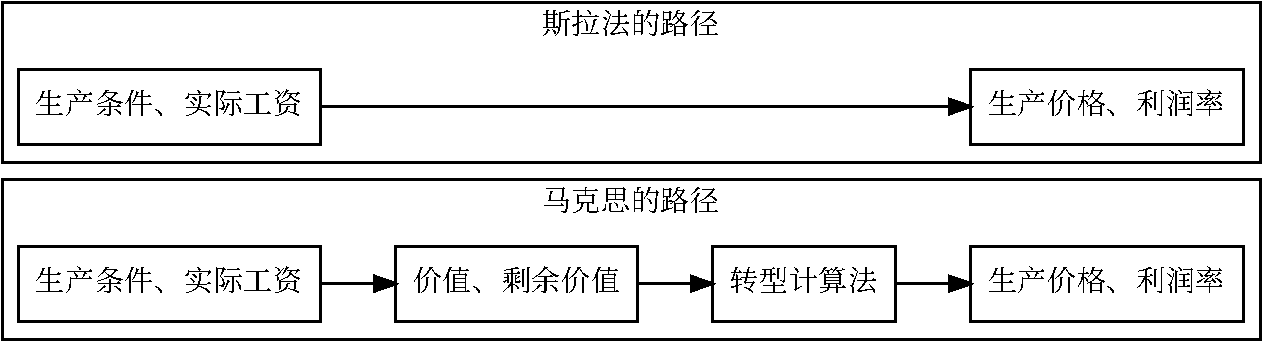
\includegraphics[width=0.8\linewidth]{data/marx1929-1990/sraffa1} 
\label{fig:sraffa1}
\end{figure}

斯拉法对转型问题的“解答”,\textbf{回避了转型问题,倾向于用生产条件和收入分配的
  数据得出商品价格和利润率这一更为基本的问题来完成。}就数量价值论而言,马克思的方
法\textbf{既过分详细,又掩饰了因果关系的真正实质。}因此,米尔福特、德米特里夫、博
特凯维兹、柴田敬和萨缪尔逊,在对马克思的价值具有逻辑上的优先权的主张提出质疑时,
都在《用商品生产商品》中获得支持他们观点的强有力的根据。

斯拉法的分析同时也强化了一些早期评论家的论据,这些早期评论家曾发现马克思劳动价值
和生产价格的关系方面的其他主张也是有争议的。因此,在\textbf{奢侈品的生产与利润率
  的决定毫不相关}方面,博特凯维兹对李嘉图的捍卫和对马克思的批判是正确的。斯拉法同
时也证实了博特凯维兹的论据,即\textbf{一般而言,利润率不能由马克思的公
  式$\sfrac{s}{c+v}$来表示;证实了肯尼思·梅提出的把价值总计为$c,v和s$是不合适的
  观点;证实了杜冈—巴拉诺夫斯基对马克思利润率下降规律的批判;}还证实了勒尔如下的
谴责,即一旦允许有\textbf{两种生产过程}存在的话,从逻辑上看,是\textbf{劳动价值依
  赖于价格},而不是相反。尽管所有这些批判都很有力量,但斯拉法的分析远远超过了其他
评论家的著作所作出的严格确证。他自己的分析框架,可以用来揭示马克思价值理论中更为
基本的缺陷。\textbf{转型不仅仅是一个“复杂的迂回”,绕远路实际上被证明是不可能
  的。}而且,\textbf{即使}当马克思的扩展的路径是可行的,马克思所认为的能够由此揭
示出的\textbf{重要剥削关系并非总是能够建立起来}。也就是说,“复杂的迂回”被证明是
一个死结。这两个问题构成以下两节的主题,第4节论证了《用商品生产商品》是如何提出使
损失达到最小化的建议的。

\section{“复杂的迂回”不存在}

马克思以及后来的马克思主义经济学的评论家和捍卫者,总是把生产出来的商品的劳动价值
看作是正值。后来,\textbf{伊恩·斯蒂德曼在1975年指出,斯拉法的分析揭示了相反情况的
  存在。}这一结果是很富有戏剧性的。首先,劳动价值可能无法确定或者可能等于零,从而
马克思的转型无法进行,他的通向生产价格的路径根本不存在,只有\textbf{斯拉法的“路
  径”是唯一可行的。}其次,\textbf{劳动价值可能为负,这一点与劳动价值可能是零一起,
  反过来破坏了马克思的基本原理,}即正的利润意味着、并且被决定于正的剩余价值。然而,
实际上,一个正的利润率可以与一个负的或零剥削率联系在一起,同时,正的利润可以与负
的或零剩余价值同时并存。


\begin{table}[H]
\centering
\caption{表\ref{t:Sraffa1}中所表明的体系类型的一个数字例证}
\label{t:Sraffa4}
\begin{tabular}{@{}ccccccc@{}}
\toprule
    & \multicolumn{3}{c}{投入} &   & \multicolumn{2}{c}{产出} \\ \cmidrule(lr){2-4} \cmidrule(l){6-7} 
    & 商品1    & 商品2    & 劳动   &   & 商品1        & 商品2       \\ \midrule
过程1 & 4      & 0      & 1    & \rightarrow & 5          & 1         \\
过程2 & 0      & 6      & 1    & \rightarrow & 2          & 8         \\ \bottomrule
\end{tabular}
\end{table}

\begin{table}[H]
\centering
\caption{用价格表示的表\ref{t:Sraffa4}体系}
\label{t:Sraffa5}
\begin{tabular}{@{}l@{}}
 $\displaystyle 4p_1(1 + r) + w = 5p_1 + p_2 $\\
 $\displaystyle 6p_2(1 + r) + w = 2p_1 + 8p_2 $
\end{tabular}
\end{table}


\begin{table}[H]
\centering
\caption{用价值表示的表\ref{t:Sraffa4}体系}
\label{t:Sraffa6}
\begin{tabular}{@{}l@{}}
 $\displaystyle 4 \lambda_ 1+1=5 \lambda _1+ \lambda _2 $\\
 $\displaystyle 6 \lambda _1+1=2 \lambda _1+8 \lambda _2$
\end{tabular}
\end{table}

这些结论与直觉是相悖的。\textbf{如果所有的生产过程都使用直接劳动的话,那么产出怎
  么能不具有经过很好确定的劳动价值,而这些价值又怎么能不是正数而是其他的情况?}这
一节探讨第一个问题,下一节探讨第二个问题。我们通过提供两个分别产生不确定的劳动价
值和零劳动价值的数字例证来开始我们的分析。表\ref{t:Sraffa4}描绘了
表\ref{t:Sraffa1}所表明的斯拉法体系中的一种特殊情况。相应的价格方程列在
表\ref{t:Sraffa5}中,其中存在着一个有经济意义的均衡。假设把商品1作为价格衡量单
位(由此$p_1=1$),\textbf{假设延期支付的实际工资是一单位的商品2},那么,如
果$p_1=1,p_2=4,w=4和r=0.25$,就使均衡得以形成。然而,运用马克思的向劳动价值“迂
回”的方法,我们是无法得到这一结论的。表\ref{t:Sraffa6}是用价值表示上述体系,它导
致了不一致的方程的形成:
\begin{align*}
 \lambda _1 + \lambda _2 &=1 \\
  2\lambda _1+ 2 \lambda _2 &=1
\end{align*}

因此,劳动价值无法被计算,结果也就没有明确的价值量可以转化为生产价格。

如果某些劳动价值为零,也会得出类似的结论。这种可能性,在
表\ref{t:Sraffa7}—\ref{t:Sraffa9}中显示出来。如果再把商品1作为价格衡量的单位,假
设延期支付的实际工资是一个单位的商品2,如
果$p_1=1,p_2=\sfrac{2}{3},w=\sfrac{2}{3}和r=0.25$的话,一个有经济意义的均衡是存
在的。但是,与第一个例子一样,马克思的“复杂的迂回”是不可能的。
表\ref{t:Sraffa9}中的价值体系表明, $\lambda _1=0和 \lambda _2=1$,因此商品1的劳
动价值就消失了,同样也就没有什么可转化的了。

\begin{table}[htbp]
\centering
\caption{表\ref{t:Sraffa1}中所表明体系类型的第二个数字例证}
\label{t:Sraffa7}
\begin{tabular}{@{}ccccccc@{}}
  \toprule
  & \multicolumn{3}{c}{投入} &   & \multicolumn{2}{c}{产出} \\ \cmidrule(lr){2-4} \cmidrule(l){6-7} 
  & 商品1    & 商品2    & 劳动   &   & 商品1        & 商品2       \\ \midrule
  过程1 & 4      & 0      & 1    & \rightarrow & 5          & 1        \\
  过程2 & 0      & 12     & 1    & \rightarrow & 2          & 13        \\ \bottomrule
\end{tabular}
\end{table}

\begin{table}[htbp]
\centering
\caption{用价格表示的表\ref{t:Sraffa7}体系}
\label{t:Sraffa8}
\begin{tabular}{@{}l@{}}
 $\displaystyle 4p_1(1 + r) + w = 5p_1 + p_2 $\\
 $\displaystyle 12p_2(1 + r) + w = 2p_1 + 13p_2 $
\end{tabular}
\end{table}

\begin{table}[htbp]
\centering
\caption{用价值表示的表\ref{t:Sraffa7}体系}
\label{t:Sraffa9}
\begin{tabular}{@{}l@{}}
 $\displaystyle 4 \lambda_ 1+1=5 \lambda _1+ \lambda _2 $\\
 $\displaystyle 12 \lambda _1+1=2 \lambda _1+ 13 \lambda _2$
\end{tabular}
\end{table}

这些结论看起来非常奇怪,因为这里存在着一种\textbf{在单一产品生产过程的脉胳中考察
  劳动价值的倾向,而在这种生产过程中,不确定的劳动价值和零劳动价值是不会出现的,}这
两种情况只会出现于联合生产体系中。但是却不能将其斥为有限关联的复杂细节而不予考虑,
因为它们在任何实际的经济中都是很普通的:例如,对羊的宰杀可以产出羊毛皮、兽皮、血、
内脏和一块块的肉。为这些显然很反常的结论提供一个直观的解释同样也是可能的,如果生
产过程中使用的直接劳动量是正的,那么净产出的劳动价值必须等于这一直接劳动的总量。
表\ref{t:Sraffa4}体系中净产出是$(5-4)+(2-0)=3$个单位的商品1,再加上$(1-0)+
(8-6)=3$个单位的商品2。由于直接劳动投入是$2$,\textbf{这一净产出就必须有$2$个单位
  的总劳动价值。然而,由于每一生产过程是以相同的比例生产净产出,因此在剩余产品的
  组成部分之间分配这一劳动价值是不可能的。}

因此,\textbf{计算单个劳动价值的一个必要条件是,生产过程以不同的比例生产净产出。}在
表\ref{t:Sraffa7}中,可以看到这样的情况。在表\ref{t:Sraffa7}中,净产出
是$(5-4)+(2-0)=3$个单位的商品1和$(1-0)+(13-12)=2$个单位的商品2。但是在这种情况
下,\textbf{就商品1而言,过程2确实具有更高的生产力,而在商品2的生产上,过程1和过
  程2具有相同的生产力。}即使作为一个整体的净产出将会有等于2的劳动价值(等于该体系
中所使用的直接劳动量),\textbf{商品1的劳动价值也必须等于零}。如果我们要让总的劳动
投入不变,而把它的一部分从过程1转移到过程2,那么我们就会在商品2的生产保持不变的同
时增加商品1的生产。由于总净产出的劳动价值必须保持2不变,那么商品1的劳动价值必须是
零。

\section{马克思“迂回”的死胡同}

这一节阐述联合生产的另一个结果,该结果同样对马克思的价值理论造成了损害。即使劳动
价值是确定的和非零的,但有一些可能是\textbf{负数}。正如在
表\ref{t:Sraffa10}—\ref{t:Sraffa12}中提出的第三个数字例证所表明的那样,这一观点会
损害把剩余价值与利润联系起来的马克思的基本原理。和以前一样,假设$p_1=1$,延期支付
的实际工资等于一个单位的商品2,从表\ref{t:Sraffa11}中得出的价格均衡
是:$p_1=1,p_2=2,w=2和r=0.25$。然而,商品2的劳动价值是\textbf{负数},因为从
表\ref{t:Sraffa12}中得出$\lambda _1= 1\sfrac{1}{2}, \lambda _2=-\sfrac{1}{2}$。

\begin{table}[!htbp]
\centering
\caption{表\ref{t:Sraffa1}中所表明体系类型的第三个数字例证}
\label{t:Sraffa10}
\begin{tabular}{@{}ccccccc@{}}
  \toprule
  & \multicolumn{3}{c}{投入} &   & \multicolumn{2}{c}{产出} \\ \cmidrule(lr){2-4} \cmidrule(l){6-7} 
  & 商品1    & 商品2    & 劳动   &   & 商品1        & 商品2       \\ \midrule
  过程1 & 4      & 0      & 1    & \rightarrow & 5          & 1        \\
  过程2 & 0      & 16     & 1    & \rightarrow & 2          & 20        \\ \bottomrule
\end{tabular}
\end{table}


\begin{table}[!htbp]
\centering
\caption{用价格表示的表\ref{t:Sraffa10}体系}
\label{t:Sraffa11}
\begin{tabular}{@{}l@{}}
 $\displaystyle 4p_1(1 + r) + w = 5p_1 + p_2 $\\
 $\displaystyle 16p_2(1 + r) + w = 2p_1 + 20p_2 $
\end{tabular}
\end{table}


\begin{table}[!htbp]
\centering
\caption{用价值表示的表\ref{t:Sraffa10}体系}
\label{t:Sraffa12}
\begin{tabular}{@{}l@{}}
 $\displaystyle 4 \lambda_ 1+1=5 \lambda _1+ \lambda _2 $\\
 $\displaystyle 16 \lambda _1+1=2 \lambda _1+ 20 \lambda _2$
\end{tabular}
\end{table}

同样,这一结果看起来也很怪,但是却能容易地对之进行直观的解释。表\ref{t:Sraffa10}
体系中的净产出等于$(5-4)+(2-0) =3$个单位的商品1,加上$(1-0)+(20-16)=5$个单位的商
品2,同时\textbf{过程2对两种商品来说都确实具有更高的生产力。结果是劳动会从过程1转
  移到过程2,两种商品作为净产出就会被更多地生产出来。}然而这一更大的净产出所包含
的劳动必须同通过减少生产力较低的过程的操作而节省下来的劳动相等。而这一点只有在一
种商品的劳动价值是\textbf{负数时才是可能的}。

把前一节中的两个数字例证和刚刚讨论的这一例证综合起来,可以推导出一个\textbf{一般
  的结论:只有当净产出是由不同的生产过程按照不同的比例生产出来的时候,而且是当没
  有一个生产过程会在生产力方面起支配作用的时候,所有商品的劳动价值才是可以确定的
  和为正数。}正如我们已经看到的,\textbf{这些条件并不是价格均衡要求普遍存在
  的。}因此,生产过程以相同的比例生产净产出的模型,和一个生产过程比其他生产过程效
率更高的体系,都是完全可以接受的。特别是,一个生产过程在生产力方面占支配地位并不
意味着资本家运用的其他过程是无利可图的。\textbf{在均衡状态中,所有的过程都同样是
  有利可图的。}

就转型而言,\textbf{负的劳动价值}——不同于不确定的劳动价值和零劳动价值——\textbf{不
  需要提出特殊的困难。}用来衡量商品的单位是任意的。\textbf{因此,只要劳动价值是可
  以计算的而且是非零的,用劳动价值作为衡量单位就是可能的。}那么,价格就变成了“每
一单位劳动价值”的价格,或价格—价值比率。如果工资和一个指定的衡量价格—价值比率的
单位已知的话,那就存在一个价格和利润率的解。在劳动价值是负数的情况下,就会出现负
的投入和产出项。\textbf{然而,这仅仅表明,一个有经济意义的解答会包括非正的相应价
  格一价值比率,以致于购买和销售这些商品会包括正的支出。}

但是,现在转型还无法实现马克思所考虑的\textbf{本质问题,即要表明正的利润率源于正
  的剩余价值率。}通过计算不变资本、可变资本和剩余价值的大小,我们发现,在
表\ref{t:Sraffa10}体系中,$c_1= 6,c_2= -8,v_1= - \sfrac{1}{2},v_2= -
\sfrac{1}{2},s_1= 1 \sfrac{1}{2},s_2=1 \sfrac{1}{2}$,因此剥削率是负的,而利润
率是正的($r=0.25$)。对表\ref{t:Sraffa7}体系中的例子进行计算,可以得
出$c_1=0,c_2=12,v_1=1,v_2=1,s_1=0,s_2=0$,该体系中没有剩余价值,即使利润率同
样是正的($0.25$),剩余价值率却为零。


\begin{table}[htbp]
\centering
\caption{斯蒂德曼的例证}
\label{t:Sraffa13}
\begin{tabular}{@{}ccccccc@{}}
  \toprule
  & \multicolumn{3}{c}{投入} &   & \multicolumn{2}{c}{产出} \\ \cmidrule(lr){2-4} \cmidrule(l){6-7} 
  & 商品1    & 商品2    & 劳动   &   & 商品1        & 商品2       \\ \midrule
  过程1 & 25      & 0      & 5    & \rightarrow & 30          & 5        \\
  过程2 & 0      & 10     & 1    & \rightarrow & 3          & 12        \\ \bottomrule
\end{tabular}
\end{table}

我们也有可能会发现,拥有负的剩余价值和正的利润的生产体系(不是仅仅指一个负的剩余价
值率与一个正的利润率并存)。斯蒂德曼的最初的例子再现于表\ref{t:Sraffa13}中。假设工
资是价格衡量的单位(即$w=1$),延期支付的实际工资包括$12$个单位的商品1和$56$个单位
的商品2,那么均衡的条件是:$p_1=\sfrac{1}{3},p2=1,w=1,r=0.2$。利润总额
是$9\sfrac{1}{6}$,是正数,而剩余价值总额则等于$-1$,是负数。

因此,马克思的基本原理无法在一般意义上成立。\textbf{正的剩余价值率不是正的利润率
  的必要条件,同时正的剩余价值对正的利润来说不是必要的。}所以,一般而言,受剥削的
劳动并不是一个“\textbf{优先的具体的量}……而它有可能被看作是形成利润的最根本的源
泉。”这一点除了价值和剥削理论以外还有其他分支。劳动价值可以是不确定的、负的或为
零这一事实,使得马克思对“运动规律”的最初分析令人怀疑,因为这些规律是用总价值范
畴($c、v和s$)来表示的,而这些范畴则被假定为是已得到明确确定的正数。因此,即使不考
虑其他情况,有些总价值范畴不确定或有反常表示这种可能性,会使得人们对马克思的宏观
经济“运动规律”产生怀疑。

一个特殊的“运动规律”是认为\textbf{资本有机构成随着资本主义发展而不断提高}。针对
这一“规律”,欧内斯特·曼德尔指出:
\begin{quotation}
  资本主义生产方式内部的绝对的限制……在于这样的事实,即在机械化的最后阶段——自动
  化阶段,由于把活劳动从生产过程中排挤出去,结果剩余价值量本身必然减少。资本主义
  与完全自动化的生产是不相容的……因为它不再允许剩余价值的产生。
\end{quotation}

如果把上述观点理解为\textbf{正的剩余劳动是正的利润的必要条件的阐释的话,}那么它早
在1898年就遭到了德米特里夫的\textbf{批判},之后又遭到了斯拉法《用商品生产商品》
的\textbf{批判}。如果假设表\ref{t:Sraffa10}的数字例证中的生产过程是完全自动化的生
产过程的话,那么在每一种情况下直接劳动投入都是零,而不是一个单位。在
表\ref{t:Sraffa11}中,除了$w$项由于不再使用直接劳动而消失外,会和以前正好一样。然
而,一个正的利润率和正的均衡价格依然会存在;假设商品1是衡量单位,答案
是$p1=1,p2=0.7,和r=0.425$,\textbf{曼德尔的论据显然是错误的,它仅仅假设存在一个
  商品实物上的剩余——不管它是否是由直接劳动生产出来的——利润是正数。}

然而,该结论并没有破坏马克思关于资本主义社会所特有的剩余价值理论。根据定义,一个
完全自动化的经济是非资本主义经济,因为它不使用雇佣劳动。然而,\textbf{它确实表明
  了马克思的价值和剥削理论存在一个更加严重的问题。}即使是在不存在计算劳动价值和实
施转型的困难的非自动化经济中,马克思关于劳动力具有创造剩余价值的特性的观点也是成
问题的。例如,在这样的情况下,人们可以计算出石油系数来表明体现于每种商品中的石油
数量,而且也可以运用马克思主义经济学家传统上用于转化劳动价值的相同方法,把这些系
数“转化”为生产价格。而且“当且仅当生产出来的每一商品具有剥削的性质,利润才是正
数…… 生产中使用的每种过去生产的商品都必须能够让出这样一种剩余……以得到某
些……唾手可得的……利润。”\textbf{从这种观点来看,劳动力并没有什么特别之处},这
与马克思的观点相反。

\section{体现马克思精神实质的一个新的斯拉法迂回}

那么,从这一残骸中还能救出点什么吗?必须等到在第14章对转型问题的后斯拉法争论进行讨
论和在第15章对斯拉法本人的著作进行批判性评估之后,才能对这一问题做出全面的回答。
但在此可以概括一下《用商品生产商品》所提出的一种辩护。这一\textbf{辩护仅仅适用于
  剥削理论,而对于修补马克思主义价值理论所遭受的创伤并没有提供任何帮助。}它也没有
提到第4节结尾处明显地提出的问题。然而,由于马克思主义者可能认为价值理论是剩余价值
分析的一个主要工具,他们或许会接受第2节、第3节和第4节的批判,但仍旧认为此处所做的
分析最终会证明马克思政治经济学的核心是有根据的,因为价值理论本身是次重要的,全面
的自动化不会存在,剥削只有在与劳动力联系起来时才有意义(参见以下第14章)。而且,将
要讨论的斯拉法的观点显然是处于马克思主义的传统之中的;它涉及到了马克思的最初争论
中的一个论点,对它进行了严格详尽的研究,然后指出,如果不是从形式上来看,马克思的
这一最初阐述在内容上是正确的。

作为转型分析的一部分,马克思坚持认为:(i)一个生产过程,如果其资本有机构成与整体经
济的有机构成相等,那么该过程生产出来的商品的生产价格就将等于它的劳动价值;(ii)该
生产过程的自身条件足以确定利润率。如果把他的利润率概念和转型的方法看作是没有问题
的,那么这一命题就是正确的。通过把更通用的公式$\sfrac{s}{c+v}$的分子分母都除
以$v$就可以把马克思的利润率公式记作$\sfrac{e}{k+1}$,其中$e$表示剩余价值率,$k$表
示整个经济的资本有机构成。由于$e$在所有的部门中都是相同的,“一般”部门的资本有机
构成等于$k$,该部门的利润率(用它自己的劳动价值范畴,$c、v和s$来计算)必须等于整体
经济中普遍通行的利润率。这意味着,该部门获得的利润是它自己生产的全部剩余价值,而
且仅仅是它自己的剩余价值,因此在马克思的转型过程中,其生产价格等于它的劳动价值。

实际上,这种观点是错误的,这既是由于\textbf{马克思错误地相信利润率可以
  用$\sfrac{s}{c+v}=\sfrac{e}{k+1}$来表示,而且还由于他的转型仅仅适用于产出。然
  而,}斯拉法的分析表明,作为整体经济代用品的“一般部门”的观点,可以给出另外一种
解释,而马克思的观点也可以得到证实。在《用商品生产商品》中,斯拉法认
为,\textbf{通过对不同部门的扩张或缩减,他所考虑的任何一个生产体系的比例都可以被
  改变,而原有体系的特性保持不变。}在这一被斯拉法称之为\textbf{标准体系}的重新安
排的体系中,以下命题成立:
\begin{enumerate}
\item 每一商品的总产出,与该商品作为投入的总计使用量有着相同的比例。
\item 标准体系中的净产出与资本的比率,给出了\textbf{最大利润率},该最大化的利润率
  同样适用于该体系和拥有原有比例的体系。
\item 当把这一净产品(指的是斯拉法的标准商品)作为价格衡量单位时,标准体系中对应于
  任一工资的利润率等于原有体系中相同工资的利润率。
\item 标准商品的均衡价格将等于它的劳动价值,原有体系中的利润率,在标准体系中可以
  表示为剩余价值与资本的比率。借助于一个简单的数字例证就可以说明这些命题。
\end{enumerate}

\textbf{不进入到由联合生产引起的复杂情况中去}这么做是再容易不过了(下面第十五章将
要分析这一问题)。因此,不是使用已经提出过的例证中的一个例证,而是在
表\ref{t:Sraffa14}和\ref{t:Sraffa15}中提供一个新例子。在原有体系中,总的投入一产
出比例是不同的;商品1的比例是一个单位,它与商品2的比例是($\sfrac{45}{28.5})或者
是1.6$,与商品3的比例是($\sfrac{48}{41}$)或者是$1.2$。通过把过
程1扩大$\sfrac{4}{3}$,把过程2缩减到原有规模的$\sfrac{4}{5}$,让过程3维持原有状态
的方式,就可以把这些比例带入到标准比例中去。现在,总的投入—产出比例是相同的:$24
/ 20=36 /30=48 /40= 1.2$。

\begin{table}[htbp]
\centering
\caption{表\ref{t:Sraffa15}中的标准体系赖以建立的原有体系}
\label{t:Sraffa14}
\begin{tabular}{@{}ccccccccc@{}}
  \toprule
  & \multicolumn{4}{c}{投入} &   & \multicolumn{2}{c}{产出} \\ \cmidrule(lr){2-5} \cmidrule(l){7-9} 
  & 商品1    & 商品2  &商品3  & 劳动   &   & 商品1    & 商品2    &商品3   \\ \midrule
  过程1 & 9 & 12 & 6 & \sfrac{3}{16} & \rightarrow & 18   & 0 & 0      \\
  过程2 & 5 & 12.5 & 15 & \sfrac{5}{16} & \rightarrow & 0 & 45 & 0      \\
  过程3 & 4  & 4  & 20  & \sfrac{8}{16} & \rightarrow & 0 & 0   & 48 \\ 
  总\quad 计 & 18 & 28.5  & 41 & 1 & \rightarrow & 18 & 45   & 48 \\ \bottomrule
\end{tabular}
\end{table}


\begin{table}[htbp]
\centering
\caption{表\ref{t:Sraffa14}体系的标准体系}
\label{t:Sraffa15}
\begin{tabular}{@{}ccccccccc@{}}
  \toprule
  & \multicolumn{4}{c}{投入} &   & \multicolumn{2}{c}{产出} \\ \cmidrule(lr){2-5} \cmidrule(l){7-9} 
  & 商品1    & 商品2  &商品3  & 劳动   &   & 商品1    & 商品2    &商品3   \\ \midrule
  过程1 & 12 & 16 & 8 & \sfrac{4}{16} & \rightarrow & 24   & 0 & 0      \\
  过程2 & 4 & 10 & 12 & \sfrac{4}{16} & \rightarrow & 0 & 36 & 0      \\
  过程3 & 4  & 4  & 20  & \sfrac{8}{16} & \rightarrow & 0 & 0   & 48        \\ 
  总\quad 计 & 20 & 30  & 40 & 1 & \rightarrow & 24 & 36   & 48 \\ \bottomrule
\end{tabular}
\end{table}

斯拉法用符号($1+R$)表示的这个量,既为标准体系也为原有体系界定了最大化的利润率,就
标准体系而言,不管相对价格会发生什么变化,$R$不可能再提高了。就原有体系而言,如果
我们用表\ref{t:Sraffa2}中的价格术语来表示表\ref{t:Sraffa14}体系,并且让工资等于
零(这样,所有的净产出与利润一起增长),结果,利润率就等于$R(=0.2)$,这同样也是最大
化的利润率。更一般地来看,正如斯拉法所指出的那样,原有体系“包括着与标准体系相同
的基本方程,只是比例不同。”而且“特殊的比例无法改变……数学上的特性。”如果把标
准商品作为价格衡量单位,由此在我们的例证中$4p_1+6p_2+8p_3=1$,工资被设定在任一可
行的水平上的话,那么,由于这一特性,利润率在标准体系和原有体系中将会是相同的,用
标准体系中的范畴术语可以得出一个更简单的表述:
\begin{equation}
r=\frac{净产品—工资}{用价格表示的生产资料总量}
\end{equation}

如果斯拉法假定整个体系中使用的总劳动等于一个单位,那么
\begin{equation}
r=R(1-w)
\end{equation}
其中$w$是工资(用标准商品单位来衡量)。因此,就我们的数字例证而言,在原有体系和标准
体系两种体系中,如果$w =0.5,那么r=0.1$。

反过来,这也承认了马克思主义对利润率的描绘,任一生产体系的净产品的劳动价值必须等
于该体系中使用的直接劳动总量(参见以上第3节)。因此,在标准体系的情况下,直接劳动总
量必须等于一个单位,标准商品的价格等于其劳动价值。而且,标准体系中的利润率总是可
以表示为该体系的剩余价值与生产资料总量的劳动价值的比率。标准体系中净产品的劳动价
值可以分解为$v_s和s_s$,其中$v_s$是工资的劳动价值,$s_s$是余下的剩余价值,下
标$s$表示标准体系。标准体系中生产资料的劳动价值同样可以表示为$c_s$。因此,最大利
润率($R$)等于$\sfrac{v_s+s_s}{c_s}$。我们已知$r=R(1-w),而(1-w)$仅仅是标准体系中
净产品的比例,它趋向于利润,由此:
\begin{equation}
  r=R(1-w)=\frac{v_s+s_s}{c_s} \frac{1-v_s}{v_s+s_s} = \frac{s_s}{c_s}
\end{equation}
这是剩余劳动或者是剩余价值与雇用资本的劳动价值的比率。很显然,如果$c_s$是正数的话,
那么正的$s_s$是正的$r$的充分必要条件。把(13.3)的分子分母分别除以$v_s$得出:
\begin{equation}
r=\frac{s_s/v_s}{c_s/v_s}=\frac{e}{k}
\end{equation}
因此,马克思主义基本原理的这一观点凭借剩余价值率和利润率也得到了维护。\textbf{而
  且,由于对任一工资水平来说,标准体系中的利润率都必然等于原有体系中的利润率,那
  么原有体系中的利润率也可以表示为剩余价值与资本的比率。}

米克总结道:
\begin{quotation}
  斯拉法对其“标准”部门中利润率与生产条件之间的关系所做的精确假定,与马克思对
  其“平均资本有机构成”部门中利润率与生产条件关系所做的假定是相同的——从这一观点
  看,斯拉法的“标准部门”从本质上讲是试图用这样一种方式来界定“平均的生产条
  件”以得出与马克思一直在寻求的结论完全相同的结论。
\end{quotation}

\textbf{从这一角度看,标准体系使得资本主义体系成为透明体,使得“隐藏的东西能够显露出
来”}。当然,这也正是马克思在其所有关于价值和剥削的著作中试图达到的目的。

\section{结论}

从总体上看,斯拉法的《用商品生产商品》与马克思主义政治经济学有着\textbf{模楞两可}的
关系,在这本书中,价值理论被证明只有在\textbf{特殊情况下才是有效的},马克思自己对
其剥削理论的阐述也同样被证明不具有普遍意义。\textbf{联合生产会使这两个理论显得空
  洞,或者会得出反常的结论。}但是斯拉法没有提到质量价值论方面的问题。因此他的处理
方案是不全面的,而他自己设计的标准商品或许会拯救马克思剥削理论中的一种形式(但是,
见下面第十五章)。而且,正如我们将要在第十五章中所看到的,许多斯拉法主义者认为,由
于斯拉法的范例与马克思的范例同样处在经济学的“剩余传统”中,马克思主义经济学实际
上由于斯拉法的著作而得到了加强,因为马克思自己的特定形式的剩余经济学的缺陷被暴露
出来,并且被证明与剩余方法本身是无关的。同时,斯拉法的批判也指出了马克思经济学中
严重的局限性,而这样做就导致了整个剩余传统受到质疑,包括由马克思所发展了的特殊看
法。然而,在我们将要在第十五章讨论这些更宽泛的问题之前,我们必须讨论“斯拉法革
命”对转型问题的处理所造成的影响。



\chapter{斯拉法之后马克思的价值理论}

\section{引言}

正如前一章所指出的,斯拉法《用商品生产商品》的影响并不是直接的,最初的影响是对新
古典主义理论产生冲击,导致了20世纪60年代中期的“\textbf{剑桥之争}”。尽管这与马克
思对“庸俗经济学”的分析息息相关,但是它并没有对马克思政治经济学自身逻辑上的一致
性产生影响。直到20世纪70年代,它对马克思经济学的直接影响才开始被意识到。同时,由
弗朗西斯·塞顿和保罗·萨缪尔逊在20世纪50年代提出的问题也期待着答案(参见以上第12章)。
有待观察的是萨缪尔逊的结论能否推广为 $n$ 部门模型,以及\textbf{(如同恩格斯和其他
  人曾设想过的)价值向生产价格的转化能否被合理地看作是一个逻辑的和历史的过程}(参见
本书第一卷第3章第2节)。另外,没有解决的问题还有与评价马克思价值理论中数学模型的作
用有关的重要方法论问题,以及价值理论问题中质和量方面的相对重要性问题。

本章的大部分、但非全部,采用的是编年体的形式。下一节探讨的是(非常稀疏地)出现
于1958年和1971年间关于转型问题方面的文献,那时萨缪尔逊以其发表在《经济文献杂志》
上的一篇引起激烈争议的长文而再次加入这场争论之中。第3节概括评述了萨缪尔逊同马克思
主义批评家之间爆发的激烈论战,第4节讨论20世纪70年代中期森岛通夫和斯蒂德曼在价值分
析上的贡献的重要意义,这在以上第13章已经作过概述。森岛通夫也卷入了重新展开“历史
上的转型问题”的讨论,对此将在第4节进行评价。

从20世纪70年代末开始,出现了几种解决转型的逻辑问题的新的尝试,加上20世纪80年代间
出现的某些附加的难点,这些内容构成了第6节的主题。第7节不再按年代顺序,而是按主题
安排的,它简要地论及20世纪最后20年间涌现出来的对\textbf{劳动价值论}的一系列异议,
这些异议与转型问题并没有直接的联系。最后第8节包括20世纪90年代初支持马克思价值和剥
削理论的一些结论。然而,要注意的是,从某种程度上讲,第15章可以被理解为是这一章的
扩展性的结论。这里所探讨的一些实质的和方法论上的问题,将在第17章对“理性选择的马
克思主义”评价时再次出现。

\section{早期的贡献}

20世纪60年代,对转型文献的最重要的贡献是罗纳德·米克对斯拉法的评论,该评论在以上
第13章第5节已作了概述。除此之外,在这10年间,发表的有意义的文章甚少。迟至1973年,
莫里斯·多布还抱怨这一讨论“还留有……某种程度的限制,甚至是很深奥的;这一讨论的大
部分内容并没有在马克思的追随者和解释者中引起多大的兴趣(或者是注意),这些人已转而
集中研究危机和帝国主义问题了。

1961年,森岛通夫和塞顿都声称,转型过程可以按照\textbf{相反的方向}进行,也就是
说,\textbf{通过运用与生产条件和净产品分配有关的资料,生产价格可以决定劳动价值。}他
们从这一点得出结论,认为实证主义者对劳动价值论的异议是没有事实根据的。正如琼·罗宾
逊(和其他人)曾经提出的,价值不是一个形而上学的概念。“不管马克思的价值概念作
为‘现实’描述或者行动向导上的有用性或不相关性如何,至少从操作上讲它是有意义的。

两年以后,挪威人\textbf{利夫·约翰森}又回到世纪之交曾引起好几个著述者兴趣的一个主
题,即\textbf{把劳动价值论和边际效用分析调和起来的可能性问题}(参见本书第一卷10.5
价值分配理论)。约翰森设计了两个价格决定模型。\textbf{在第一个模型中,工人}拥有维
持生存所必需的条件,它决定了传统的马克思模型中的\textbf{均衡实际工资},\textbf{而
  资本家则使得预算约束条件下的新古典主义效用函数最大化。这时,边际效用决定的是资
  本家消费的商品的数量,而不是其价格。在第二个模型中,工人和资本家都有效用函数,
  如果没有一个单独的收入分配理论或者——约翰森提出的变形的——反映工人最低效用水平的
  详细说明的话,利润率就无法确定。现在价格间接地受到边际效用的影响,}因为工人效用
函数中的任何变化都会影响到利润率,从而改变生产价格。

塞顿1957年的那篇文章发表之后,一个在价值和剥削问题的分析中更加热衷于运用数学技术
的时代开始了。然而,起初几乎没有人对这两篇文章作出反应,同样地,置盐信雄在1963年
的一篇文章中对转型问题所做的相当关键的评论,也没有引起任何反应,人们仅仅记住了它
对马克思利润率下降原理的攻击(参见第7章第3节)。在由萨缪尔逊挑起的争论开始之前,另
一本重要的著作是安德拉斯·布罗迪的《平衡、价格和计划》,该书先用匈牙利文出
版,1970年又以英文再版。正如我们将在以下第5节和第6节所看到的,布罗迪预测到了后来
争论的若干方面的问题。但是他的著作在西方没有造成多少直接的影响,恐怕在东方造成的
影响会更小,因为在东方,有创造性的知识分子的努力仍旧碰到到巨大的障碍。

在这些年里,米克对斯拉法的解释大部分被忽视了,只有一个有意义的例外:斯拉法在剑桥
的同事\textbf{莫里斯·多布},开始同他本人的许多共产主义同事分离开来,这是由于他坚
持认为,\textbf{《用商品生产商品》对马克思作了证明},这个证明不亚于该书对新古典主
义经济学诅咒似的控告。在1970年发表于荷兰《经济学家》杂志上的一篇非常有影响的文章
中,多布把斯拉法置于\textbf{古典的传统}之中,他认为这一古典的传统包括卡尔·马克思
以及博特凯维兹和德米特里夫(参见本书第一卷第3章第4节和第5节)。这一切都表
明,\textbf{利润率依赖于投入生产部门的生产条件(不管是工资品还是不变资本的组成要
  素),并且只能依赖于这些生产条件。}多布强调,在与马克思不一致的关于分配理论的少
数几篇评论中,斯拉法没有提供什么东西。\textbf{在斯拉法的模型中,资本家对生产资料
  的垄断是固有的,甚至他把工资当作是剩余产品的组成部分的作法,也可以看作是对现代
  资本主义状况的符合实际的反映。。}

多布在其最后一本书中,对这些观点做了进一步阐述,他重点介绍了斯拉法、古典经济学家
和马克思之间在方法论上的相似性。\textbf{所有这些人都认为,从逻辑上
  看,\CJKunderdot{分配独立于交换},在任何情况下,价格都是取决于收入分配(再加上生
  产条件),而不是相反。}这一“前杰文斯决定规则或模式”使他们的观点同新古典主义理
论家的观点非常明显地区别开来。。以下第15章将对这一在经济思想史上非常有影响力的解
释进行评价。

\section{萨缪尔逊争论}

1969年或者是1970年,萨缪尔逊从美国国家科学基金获得津贴,资助他对马克思价值理论的
研究。第二年他发表了他的这一研究成果的初步概要。他的一篇较长的论文于1971年发表在
《经济文献杂志》上。。萨缪尔逊的结论主要还是他在1957年就已得出的那些结论(参见以上
第12章第2节)。劳动价值理论是一个复杂的迂回;生产价格和一般利润率可以直接地取决于
与生产条件和收入分配有关的信息;因此,马克思的剩余价值理论对于理解资本主义经济中
的利润来说是不必要的。

萨缪尔逊早期的文章虽然被马克思主义经济学家所忽视,但1971年发表的这篇文章却引起了
一场激烈的争论。这种批判性反应上的不同,可以举出好几个理由。对马克思主义的一般性
兴趣增强了,而且同以前相比,有更多的马克思主义经济学家以学术研究为专职。《经济文
献杂志》与更加令人生畏的《美国经济评论》相比,其专门性不太强,但却有更多的读者。
到了1971年,萨缪尔逊已成为正统经济学的一个起统率作用的人物,与20世纪50年相比,他
有了一个更高大的公众形象。1970年,他获得了诺贝尔奖,各种介绍他的著作版本,在销售
量上已远远地超过其他以英文出版的经济学著作。全世界的一届届的大学生从萨缪尔逊的
《经济学》中学到了他们最基础的理论。最后,还有一个风格问题。1957年发表的文章在语
气是上有节制的,而且还带着学术的腔调,但是1971年发表的文章的大部分则相反,而且带
有(并且是蓄意的?)挑衅。
\begin{quotation}
  当你穿越代数学的迷宫,开始理解正在发生的事情时,你发现“转型的算法”可以精确地
  表述为下述形式:“\textbf{反复思考两种可以替换但却又不一致的体系,写下一个。现
    在通过用一个橡皮把它擦掉来进行转型,然后再填上另一个。如此你就完成了转型的算
    法。}”运用这一技术,可以进行从燃素到熵、从托勒密到哥白尼、从牛顿到爱因斯坦、
  从《创世纪》到达尔文的转型——然后是从熵到燃素的转型……这种无可争议的无聊真理,
  在目前已持续34个世纪的冗长文献中的任何地方都没有得到强调,这告诉我们需要对转型
  问题进行系统的考察研究。
\end{quotation}

正是这一“\textbf{橡皮原理}”而不是其他东西,激怒了马克思主义读者。当时的《经济文
献杂志》编辑,马克·珀尔曼,很快收到了大量批判性的短文和评论。他的反应相当迟钝。同
意出版的那些仅有的投稿,均来自于杰出的\textbf{学院式经济学家}。在两篇相当筒短的投
稿中,阿巴·勒纳异乎寻常地指责萨缪尔逊“对如此彻头彻尾地遭到破坏的劳动价值论作了无
根据的让步”;而\textbf{琼·罗宾逊则声称萨缪尔逊对古典马克思主义和新古典主义模型进
  行了折衷。威廉·鲍莫尔}则认为,萨缪尔逊误解了马克思的意图,马克思
\begin{quotation}
  主要关注的是\textbf{利润和剩余价值}之间的关系,仅仅偶尔(作为达到前者的工
  具)关注\textbf{价格和价值的关系}……似乎显示出土地是地租的源泉,资本是利润和利
  息的源泉的竞争过程,仅仅是一个\textbf{分配现象},它掩盖了劳动才是产出的唯一有社
  会关联的源泉的事实。这正是马克思的劳动价值论和转型问题分析的重要意义。
\end{quotation}

萨缪尔逊否认这一点,相反强调他的“擦除和取代原理”同样适用于剩余价值向利润的转化。
鲍莫尔反击说他的文章是致力于研究马克思的目标的本质,而不是研究他是成功还是失败这
一不同的问题。最后,森岛通夫对他于1973年正值辩论高峰期出版的著作《马克思的经济学》
进行了捍卫。他相信他对马克思的批评比萨缪尔逊的批评更严厉,然而还是提供了马克思的
基本观点能够得以保留的论据。

这些投稿没有一篇是特别深刻的,但是以后投往《经济文献杂志》的一系列评论却没有发表。
珀尔曼反而任命马丁·布朗芬布伦纳去“对那些未正式介入新近一轮‘马克思主义——现代主
义’论争的经济学家进行概述”。他的概要是否包括六篇被拒绝发表的文章的摘要并不很清
楚,但这正是他所提供的。他指出,他们的腔调从“学术式的到漫骂式的。”从布朗芬布伦
纳的描述来看,似乎只有一篇文章明确采取的是新古典主义观点,有四篇是试图对马克思的
价值理论进行捍卫。很显然,珀尔曼对发表文章的选择并不是不偏不倚的,而且萨缪尔逊在
一部分标题为“引证的著述者的反应”栏目中发现,该栏目“对那些没有被同意发表的夭折
文章所进行的评论有些零散。”

有两篇曾遭到拒绝的文章后来在别处发表了。资深议会共产主义者\textbf{保罗·马蒂克},
提出了三个实质性的观点。第一,\textbf{他(正确地)强调马克思的价值理论与资产阶级均
  衡分析共同具有成为一个“理论装置”或“思想结构”的特性,因此,马克思的价值理论
  不能被直接观察到。}第二,他认为马克思主要关心的问题是“\textbf{为什么社会劳动关
  系是以价值关系表现出来?”马克思曾经提出“价值概念怎样才能全部呈现出来”(首
  先?)。}他发现答案就在资本主义生产方式的特殊阶级关系中。这里暗含着价值理论质的方
面和量的方面之间的一个区别,这一区别既构成萨缪尔逊其他方面批判的主要特色,又被用
来反对马克思的斯拉法主义批判家(参见以下第15章)。第三,马蒂克认为,\textbf{劳动价
  值论只有在整体经济的水平上才能得以证实:“价值规律不是在每天的价格关系中得到证
  明,而是在生产价格的总体升降过程中找到经验证明的……该体系作为一个整体对价值分
  析是敏感的。}”森岛通夫在后来得出了一个更加严格的相关结论(参见以下第4节)。马蒂
克坚持认为,萨缪尔逊对此一无所知,他是一个庸俗经济学家;他的代数学是“夸大的垃
圾”,他“浪费了自己的时间和国家社会基金会的金钱。”

如果马蒂克是把学术腔调和漫骂口气结合在一起的话,那么\textbf{戴维·利伯曼}对萨缪尔
逊的攻击则采取一种严谨的模式。利伯曼首先提出了他自已解决\textbf{转型问题的几何学
  方案},该方案\textbf{取消了传统的不变条件},包括价格总额与价值总额相等和(或)剩
余价值总额与利润总额相等,\textbf{要求剥削率不管是用价值表示还是用价格表示都要相
  同}。利伯曼为这一修正提供的正当理由是:工人与资本家是围绕着剥削率而不是利润率而
展开阶级斗争的。跟马蒂克一样,利伯曼也抱怨萨缪尔逊仅仅探讨了该问题的\textbf{量的
  方面},而忽视了更有意义的\textbf{质的方面}。萨缪尔逊完全无法理解“\textbf{价值
  问题是一个社会范畴}”,因此“在马克思主义意义上说”,他自我暴露为“\textbf{一个
  可怕的政治的经济学家}”。利伯曼总结道:“为了推进争论中他这一方的发展,(萨缪尔
逊)必须跨越‘哲学—社会学’和‘经济分析’之间的随意界限,以面对作为社会关系范畴的
价值的定义”。

\textbf{价值质的问题和量的问题}之间的这一关键性区别首先起源于马克思的分析,斯威齐
在其著作《资本主义发展论》中对此作了强调。\textbf{1975年霍华德和金提出},应该把这
一区别有效地应用于收入分配的分析中,而这一点实际上包含在了鲍莫尔对萨缪尔逊的批判
中。在对利伯曼当时未发表的文章所做的(必要的)简短评论中,萨缪尔逊把整个观点看作是
包括“一个几乎是滑稽可笑的拜物教和双关语”的错误概念而不予考虑。这是完全不正确的。
萨缪尔逊的错误可能在于:\textbf{通过把洗澡水(量的方面)和孩子(质的方面)一起倒掉而
  弱化了他自己分析的影响力。}实际上,对价值的这两方面\textbf{在逻辑上是分离的}问
题可以作出强有力的证明。如果真是这样的话,那么在取消——按照萨缪尔逊的理由——马克思
数量价值理论的同时接受其对质量问题分析的本质是可能的。利伯曼拒绝这一结论,斯威齐
最终对此也是畏缩不前,但是它却吸引了一些不太教条的捍卫者,他们认为质量价值理论与
斯拉法主义者和马克思主义者之间和平共处的明显承诺之间,存在着持续的关联性(参见以下
第15章)。

马蒂克并不是把萨缪尔逊当作是庸俗经济学家的唯一的评论家,他自己坚决否认这一指
责:“在这一讨论中我的优势之处不是新古典的,而是\textbf{斯拉法}的!……我所说的是
非新古典主义者\textbf{琼·罗宾逊}一直在说的”。萨缪尔逊也不否定传统的分配理论,只
是拒绝与之站在一起。他所希望做的就是打破把马克思看作是一个预言家的神话,他揭露
了“藏在事物表面之下的无法服从于传统政治经济学的秘密。”正如我们已经看到的,在这
一方面,他只是部分地成功了,因为他没有认识到价值理论质的方面的重要性。然而,在这
场论战的最后,\textbf{萨缪尔逊}确实从他1971年的攻击中\textbf{退却了一点},减弱了
他对“橡皮原理”的固执,把马克思描述成为“\textbf{一个政治经济学最初的有创造力的
  缔造者}”。

\section{森岛通夫和斯蒂德曼加入论战}

与此同时,在大西洋彼岸也进行着一场激烈的争论。这场争论首先集中在莫里斯·多布对古典
马克思主义综合的认同上(参见以上第2节)。多布是英国马克思主义经济学家的老前辈,是英
国共产党最重要的理论家(尽管偶尔也持异议),也是斯拉法在剑桥的密友,鉴于斯拉法对由
他的著作引起的争论持绝对沉默态度,多布对其观点的解释迅速成为典范的形式,多布本人
也成为正统马克思主义捍卫者攻击的主要对象。

攻击的最初阶段是在新成立的杂志\textbf{《经济与社会》}上展开的,其中首先是杰夫·皮
林接着是苏珊娜·德·布隆豪夫,对李嘉图的价值理论和马克思的价值理论之间的主要区别进
行了鉴别。他们认为,李嘉图的方法与马克思的方法截然不同,这表现在辩证法、矛盾、历
史特殊性,以及形式和内容之间、本质和现象之间、质和量之间的区别等各个方
面。\textbf{马克思的概念是独一无二的;}在古典政治经济学中找不到他对使用价值和交换
价值、抽象劳动和具体劳动的分析的对等物。首要的是,正如马克思已经认识到
的,\textbf{李嘉图由于混淆了价格和价值而受到批判。}因此,多布对价值理论中“古典马
克思主义”传统的发明是相当错误的。

多布的同事\textbf{鲍勃·罗松}在对他称之为\textbf{剑桥学派、英国—意大利学派或“新李
  嘉图”学派}的一个广为人知的\textbf{批判}中,(从一个稍微不同的角度)得出了类似的
结论。(现在更一般的提法是\textbf{“斯拉法”}学派。)罗松特别不赞成把马克思理解
为“仿佛他是一个英国古典经济学家”。\textbf{实际上,马克思早已对李嘉图把剩余价值
  仅仅看作是一个单纯的分配现象的观点进行了攻击,正是这一观点导致李嘉图忽视了生产
  过程。}同时,马克思也批判李嘉图混淆了劳动力和劳动,批判他无法区分\textbf{不变资
  本和可变资本}。罗松强调,由于受到李嘉图分析的影响,新李嘉图主义者无法理解马克思
的生产方式概念,因此夸大了生产的技术方面,而牺牲了它的\textbf{社会方面},把生产看
成是“一个非社会的或自然的过程”。由于新李嘉图主义的代数学与几种不同的生产方式都
一致,因此就无法验证马克思主义\textbf{关键的历史性特征}。真正的危险在于,马克思主
义者会陷入一场\textbf{争论的束缚}中,这场争论所参照的条件一方面由诸如庞巴维克这样
的庸俗经济学家,另一方面由诸如博特凯维兹这样的新李嘉图主义者来规定。。

\textbf{罗纳德·米克}在其著作《劳动价值论研究》第二版(1973年)的长篇的导言中,已对
这些观点所存在的弱点进行了证实,他展示了怎样使斯拉法的高度抽象的再生产模型变得具
有\textbf{历史和社会的具体性}。米克运用马克思的“逻辑—历史的方法”,对一系列斯拉
法模型作了系统阐述,从简单商品生产开始,从不同部门具有不同利润率的早期资本主义阶
段成功地过渡到《资本论》第三卷所描绘的单一利润率普遍通行的成熟资本主义阶段。米克
总结道,\textbf{斯拉法不情愿以这种方式提出他自己观点的做法,并没有使他成为一个庸
  俗经济学家,也没有使分析价值和剥削理论的统一的古典马思主义方法变得无效。}

在这一点上,森岛通夫将其杰出的才华倾注在马克思主义经济学的研究上。除了布罗迪的文
章以外,\textbf{森岛通夫出版于1973年的《马克思的经济学》,是第一部用数学语言分析
  这一主题的长篇著作},接着就是在《计量经济学》上发表的一篇有着同样难度的文章,再
后来是与乔治·凯特福斯合著的关于这些观点的更为流行的一篇文章。森岛通夫似乎成了系统
探索由联合生产、固定资本和存在可替换生产过程所提出的劳动价值论问题涵义的第一人。
正如马克思所理解的,\textbf{在某些情况下劳动价值可能是负的或不确定的}(参见第13章
第4节),更多地受诺伊曼的而不是受斯拉法的影响,森岛通夫认为,\textbf{通过把一个商
  品的价值重新界定为生产它所需要的最小劳动量,这些困难能够被克服,而且也才能被克
  服。}当按照这些\textbf{“真实”或“最优价值”}来计算必要劳动和剩余劳动的时
候——而且\textbf{只有在这个时候}——森岛通夫所说的“马克思主义基本原理”\textbf{才能
  够普遍地成立:一个正的剥削率必须有一个正的利润率,反过来也是这样。}

从马克思主义角度出发,对这一点所持的\textbf{异议是双重的}。很显然,\textbf{这并不
  是马克思用来界定价值的方式}(它也不可能是马克思用来界定价值的方式,因为在马克思
生活的年代,相关的数学方法还没有发明出来。)而且更重要的是,\textbf{森岛通夫的“真
  实价值”是非加总的,这意味着不再有可能把商品界定为体现于商品中的不变资本、可变
  资本和剩余价值之和。}但是,马克思的许多最著名的观点,都是建立在价值确实是加总的
这一假定之上的,而且他还认为这一加总的特点太明显而无需加以证明。例如,一旦加总的
价值被取消的话,《资本论》第二卷的再生产模型就必须重新表述。因此,森岛通夫用冯·诺
伊曼的方式对马克思主义经济学的重新铸造具有远远超过价值和剥削理论的许多分枝。而且,
尽管森岛通夫已经表明在联合生产的条件下,马克思主义基本原理还是有可能得到保留,但
是他没有这样做的欲望,更不用说这样做的必要性了。换句话说,森岛通夫的价值分析自身
也可能仍旧被看作是一个“\textbf{复杂的迂回}”。

\textbf{伊恩·斯蒂德曼}不久就颇具说服力地把这些问题提了出来。斯蒂德曼在1975年发表
在《经济学杂志》上的一篇论文(参见以上第13章)中承认,如果运用森岛通夫
的“\textbf{真实价值}”的话,负的剩余价值与正的利润之间的矛盾就可以避免了。但
是,\textbf{却没有使人非相信不可的理由去这样做。}斯蒂德曼在他的《斯拉法之后的马克
思》一书中认为,“凡是可以用价值量来表示的任一事物,\textbf{不用价值量也可以表示
  出来,因为价值量仅仅是更基本的物质生产条件和实际工资的派生物。}”斯蒂德曼(挑衅
性地)总结道:“可以毫不过分地强调,只有在对后者的信奉是前者发展首要束缚的否定意义
上,为资本主义社会提供一个唯物主义描述的方案才会依赖于马克思的价值分析。”尽管这
一结论来自于一个马克思主义者,他曾在《社会主义经济学家会议公报》和《新左派评论》
上论证过他的观点,但正如几个评论家所提到的,这一结论实际上与萨缪尔逊
的“\textbf{橡皮原理}”是一致的。

那么,\textbf{“斯拉法之后”的马克思还剩下些什么呢?对森岛通夫和凯特福斯来说,}剩
下的就是用森岛通夫的“真实价值”表述的马克思主义基本原理,\textbf{即用剩余劳动解
  释利润。}斯蒂德曼的学生\textbf{杰夫·霍奇森}声称,即使是这一点也是\textbf{多余
  的},因为\textbf{具体劳动概念本身“仅仅是一个隐喻,在任一社会现实和与此相对应的
  现象形式中都缺乏物质基础。”}对\textbf{霍奇森}来说,\textbf{利润的真正基础
  是“用其价格计算”的剩余产品。}在《斯拉法之后的马克思》中,斯蒂德曼认为,斯拉法
的贡献在于为森岛通夫用“真实价值”表述马克思主义基本原理提供了一个基
础。\textbf{但是两年以后,斯蒂德曼追随霍奇森,而不是森岛通夫,否认剩余价值或剩余
  劳动能够解释利润的存在。}它们是“测量剩余[产品]的两种方法…… \textbf{(狭义
  的)剥削的存在和利润的存在仅仅是同一枚硬币的两面,它们仅仅是存在着物质剩余这样一
  个事实的‘劳动’和‘货币’表述。}”

\section{回到“历史上的转型问题”}

几年前,\textbf{安德拉斯·布罗迪}曾针对斯威齐关于“为什么不从价格开始?”的提问,作
出了一个黑格尔式的回答。\textbf{对黑格尔来说,“一种事物的历史就是该事物自身”,
  因此,“我们的观点和范畴是真实过程的反映,按照它们在历史上出现的顺序来展开它们
  是有好处的”。}用马克思的话说,\textbf{由于价值“不仅在理论上而且在历史上优先于
  生产价格”,}因此,如果要切合实际地谈论价格和利润的话,从价值和剩余价值分析开始
是必然的。以后的一些著述者声称,森岛通夫和萨缪尔逊对“历史上的转型问题”的忽视,
反映了他们各自观点中的主要缺陷。

马克思去世后,恩格斯对转型问题的历史方面进行了详细的分析,之后鲁道夫·希法亭又对之
进行了捍卫(参见本书第一卷第3章第2—3节)。在现代的著述者中,\textbf{罗纳德·米克}对
这一问题强调的最多,因为他把这一解答看作是对马克思的\textbf{逻辑—历史方法}的最重
要的证明。米克强调,\textbf{劳动价值论的地位在马克思所概括的每一个不同历史阶段是
  不相同的。}在没有商品生产的社会里,根本不存在交换,因此价值问题就没有被提出来;
或者会发生零星的物物交换,其中的交换比率也是相当偶然的。在这一阶段,价值理论是不
相干的。第二阶段是\textbf{简单商品生产阶段。}在这一阶段,\textbf{劳动价值论无限制
  地适用。在早期资本主义阶段,由于竞争力太弱,无法在所有部门间形成均衡的利润率,
  在这一阶段劳动价值论也是无限制地适用。}然而,到了\textbf{成熟的资本主义阶段,自
  由竞争形成了统一的利润率,正是在这第四阶段,系统地区别于劳动价值的生产价格出现
  了。}最后,\textbf{在后资本主义(社会主义或共产主义)社会,商品生产将被取消,对任
  一价值理论的需求也将随之取消。}按照以上定义,“价值”和“生产价
格”都是\textbf{具体的历史范畴,}而且作为一个历史过程,从前者向后者的转型,产生于
从早期资本主义向成熟资本主义过渡期间。

如以上所证实的,\textbf{森岛通夫和凯特福斯}1975年发表在《经济学杂志》的文章中,对
上述观点提出了\textbf{第一个决定性的挑战}。(70年代中期在这一杂志上允许发表的有关
价值和剥削论文的数量,比在此之前和在此之后发表的数量都多。)森岛通夫和凯特福斯提出
这样一个问题:“什么时代是价值时代?”他们认为,\textbf{简单商品生产不可能是价值时
  代,这既有历史的原因也有逻辑的原因。}从历史上看,即使是在西欧封建社会瓦解的时期,
也从来没有存在过这样一种生产方式。在这一时期,还残存着某些封建经济关系,而当时自
给自足生产的持续重要性和劳动的明显不流动性表明,\textbf{商品生产的发展是不完善
  的。}而且,简单商品生产从逻辑上讲也是不可能的,因为\textbf{抽象劳动这一重要概念
  预先假定要压制对任一劳动的偏好,而没有抽象劳动,价值理论是不适用的。这只有在资
  本主义条件下才会发生。}

那么,“价值时代”是不是对应于米克所说的早期资本主义呢?森岛通夫和凯特福斯也否认
了这一点。他们认为,\textbf{米克的分析忽略了代表着封建主义和工业资本主义之间这一
  阶段的商业资本。商人的利润来自于不等价交换而不是等价交换。很显然,劳动价值论无
  法适用于此。}工业资本的产生包含商人对其活功的扩展,首先是在生产(或家庭)体系中做
承包商,以后是建立工厂。很显然,在这一历史过程中,商品根本不是按照反映其劳动价值
的价格来进行交换。森岛通夫和凯特福斯总结说,\textbf{马克思曾打算把简单商品生产作
  为一个理想的模式或“逻辑表象”,用来说明利润的出现。}这对前资本主义经济中的价格
决定来说没什么意义。\textbf{实际上,商品从来都没有按照它们的劳动价值来出售,转型
  问题应该被看作是一个纯粹的逻辑问题,它的解答从本质上讲成了“一个静止的、永恒的
  分析手段”。}

尽管米克对自己的观点作了捍卫,但是没有什么用处。之后对转型问题的历史地位进行证明
的尝试很少而且是不成功的。\textbf{从转型问题争论方面可以得出三个一般性的结论。第
  一,将“逻辑的—历史的”方法运用于价值理论并不像米克所讲的那么容易;第二,还存在
  这样一种情况,即“我们对在交换和成本与收益的计算还不普遍的社会中的分配和定价了
  解很少”;第三,也是最重要的,借助于价值对价格的历史优先性,是无法挽救(数量)劳
  动价值论的。}

\section{再次提及转型的逻辑}

转型问题具有多面的性质现在是很明显的了。到20世纪70年代末,它已成为各种历史和逻辑
背景下关于价值与价格数量关系的一整套问题。数量理论也充满了对质的思考,在这方面存
在着种种看法和相互的误解。而且,尽管在历史的转型方面,在联合生产、固定资本和可选
择的生产过程的内涵方面,在造成“复杂迂回”的功过(或必然性)方面,还存在着各种各样
的争论;尽管存在着上述所有的情况,讨论的最后结论,还必须提到马克思最初在《资本论》
第三卷介绍的简单的、一种商品、一种生产过程模型中提出的问题。

试图维护马克思的第一个(也是最不成功的)尝试来自于安瓦·赛克,他认为,正如普遍被相信
的,马克思自己的转型过程并没有错,但最好是把它看作是一个重复过程的第一阶段,从这
个过程中最终会产生正确的(博特凯维兹的)生产价格。也就是说,《资本论》第三卷中得出
的价格应该仅仅被看作是一个最初的近似值,应该用相同的算法首先对它们进行计算,然后
再计算“第二阶段”的价格,等等,这样就可以逐渐地达到博特凯维兹的解答。尽管塞克的
观点在当时引起了巨大的轰动,并且至少得到保罗·斯威齐这样的人物的认可,但是他的观点
既不新颖,也不令人信服。在乔治·冯·查洛索夫1914年前的文章中就发现类似观点的萌芽(参
见以上第12章第2节),而当时布罗迪和森岛通夫都曾预先将马尔可夫矩阵应用于转型问题。
正如\textbf{森岛通夫}所提到的,困难在于\textbf{最初的起点是随意的}。霍奇森相当尖
刻地指出,即使不是开始于劳动价值,而是开始于“商品名字在被翻译成塞尔维亚—克罗地亚
语时包含的字母数量”,塞克的复杂过程最终也能够得出一个确切的生产价格的近似值。萨
缪尔逊在瓦西里·里昂惕夫的激励下,也早已设计了一个类似的毫无意义的“莫名其妙”的价
格模型。

更有趣的是亨特和格利克在《新帕尔格雷夫辞典》关于转型问题条目上称作的“\textbf{新
  的解答}”。这一解答首先由法国的G·迪梅尼尔在1980年公开提出,而美国经济学
家\textbf{邓肯·弗利}一直在沿着相同的思路工作,而且他们的观点自此一直得到其他人的
支持。弗利在其《理解资本》一书中作出了最易于理解的描述。假设一个两部门经济,运用
钢和人类劳动生产钢和小麦,在下述条件下:
\begin{align*}
\sfrac{1}{2}钢+ 1劳动 &\rightarrow 1钢 \\
\sfrac{1}{4}钢+ 1劳动 &\rightarrow 1小麦
\end{align*}
钢和小麦的劳动价值( $\lambda _s$)和( $\lambda _w$)可以用与以前例证中所使用的方式
相同的方式计算出来:
\begin{align*}
\sfrac{1}{2}\lambda _s+1 &= \lambda _s \label{e:after1} \\
\sfrac{1}{4}\lambda _s+1 &= \lambda _w
\end{align*}
得出 $\lambda _s=2和 \lambda _w=1.5$。弗利\textbf{假设货币的价值(在该体系之外产
  生)是一个单位,货币工资是$0.5$。}如果工人仅仅消费小麦,这样他们能够购
买$0.5 \times 1.5=0.33$个单位的小麦。

价值体系现在可以表述如下:
\begin{equation*}
  \begin{array}{*{7}{c}}
  \toprule
  & c & v & s & c+ v+s & e=s/v (\%) & r= s/(c+v) (\%) \\
  \midrule
  钢  & 1 & \sfrac{1}{2} & \sfrac{1}{2} & 2 & 100 & 33\sfrac{1}{3} \\
  小麦  & \sfrac{1}{2} & \sfrac{1}{2} & \sfrac{1}{2} & 1\sfrac{1}{2} & 100 & 50 \\
  总计/平均  & 1\sfrac{1}{2} & 1 & 1 & 3\sfrac{1}{2} & 100 & 40 \\
  \bottomrule
\end{array}
\end{equation*}

(注意,该经济\textbf{不是处于简单再生产的状态下,因为钢的产出量已超过了这两个部门
  所使用的钢的投入量。})要把这些量转化为\textbf{生产价格},弗利提出了\textbf{两个
  重要的假定},这两个假定构成了“新的解答”的\textbf{不变条件}。第一个假定是
让\textbf{价值总额等于价格总额,但这仅仅是针对净产品而言的}(而马克思和博特凯维兹
则坚持这一条件适用于总产品)。第二个假定是\textbf{要求可变资本转型过程中要保持不
  变。}实际上,弗利对劳动力价值进行了\textbf{重新界定}:它\textbf{不再是包含在工
  人所消费的一系列工资品中的劳动,而是货币工资与货币价值\footnote{弗利所说的货币
    价值是在商品生产中耗费的总劳动时间与总增加价值的比率。}的乘积。}那
么,\textbf{价格关系}可以表达如下:
\begin{equation}
  \label{e:after2}
  \begin{aligned}
    (\sfrac{1}{2}p_s + \sfrac{1}{2})(1+r)=p_s \\
    (\sfrac{1}{4}p_s+\sfrac{1}{2})(1+r)=p_w \\
    (p_s-\sfrac{1}{2}p_s) + (p_w- \sfrac{1}{4}p_s)=2
  \end{aligned}
\end{equation}
其中第三个方程使得用价格表示的净产品(左边)和用价值表示的净产品(右边)相
等。\eqref{e:after2}的答案是$p_s=2.208,p_w =1.448和r=37.65\%$,给出如下的价格体
系:
\begin{equation*}
  \begin{array}{*{6}{c}}
  \toprule
  & 不变资本 & 可变资本 & 利润 & 生产价格 & 利润率 (\%)  \\
  \midrule
  钢  & 1.104 & 0.5 & 0.604 & 2.208 & 37.65  \\
  小麦 & 0.552 & 0.5 & 0.396 & 1.448 & 37.65 \\
  总计/平均  & 1.656 & 1 & 1 & 3.656 & 37.65 \\
  \bottomrule
\end{array}
\end{equation*}

“\textbf{新的解答}”的特征是很容易确认的,\textbf{用价值和用价格表示的净产品是一
  样的}($=2$);\textbf{可变资本也是不变的}($=1$)。由此可以得出\textbf{马克思的一
  个不变条件得到满足,因为剩余价值总额等于利润总额}($=1$);整个体系中的剥削率也不
变($=100\%$)。但是钢产品的价值($3.5$)\textbf{低于}其价格($3.656$);用价值表示的不
变资本($=2$)\textbf{低于}用价格表示的不变资本($=2.208$);价值体系中的利润
率($=33.3\%$)低于价格体系中的利润率($=37. 65\%$)。这最后的差异当然曾令马克思非常
焦虑。\textbf{而且转型过程还包含了实际工资的增加},因为工人现在可以购买$0.5
\times 1.448=0.345$个单位的小麦,而不是$0.33$个单位的小麦。\textbf{这意味着价值在
  逻辑上优先于价格的假定已不存在:“分配的假定要求事后的知识,实际的价格体系必须
  在工资率确定之前就是已知的,人们不能一步步地从价值进入到价格。这两个领域必须单
  独加以考虑,而新解答则仅仅提供了从一个领域到另一个领域的详细过程。”}最后,人们
还必须记住,\textbf{这是一个单一产品、单一过程的模型,在这一模型中,还没有遇到由
  联合生产、固定资本和可替换生产方法提出的问题。}总之,“新的解答”在处理转型问题
上与更传统的方法相比是否有了真正的发展还是令人疑虑的;而且两者都没有克服萨缪尔森
提出的运用价值范畴是一个\textbf{复杂的迂回}的指责。

\textbf{所有这一切纯粹是静止的,}也就是说,它所关注的是一个“均衡”利润率和“均
衡”生产价格的特性,\textbf{而不是这些均衡量在竞争资本主义经济中得以建立的过程。马
克思似乎再一次把资本为了寻求更高的利润而在部门间自由转移直到形成一个普遍的一般利
润率看作是不证自明的,尽管他意识到这可能包含着相当多的干扰。}然而,到了20世纪80年
代,事情显然地变得比这更复杂了。

\textbf{伊曼纽尔·法尔约恩和摩舍·马克沃夫}同时提出了这一问题,而H·尼卡多则以非常不
同的方式提出了这一问题。法尔约恩和马克沃夫列举了一系列令人印象深刻的论据支持他们
自己的观点:即\textbf{利润率实际上是极不相等的,即使在部门内部也是如此,而且“等
  价规律”从经验上讲也是错误的。}他们认为,这是\textbf{资本主义竞争过程本身的必然
  结果}:“在对竞争概念某些合理推理的条件下,\textbf{试图推动利润率远离均衡的力量,
  至少与那些推动利润率趋向均衡的力量一样真实、有力。}”这些力量包括技术的不平衡发
展,以及使用掠夺性的低定价战略使竞争者破产的方式,保证长期高额利润。
\begin{quotation}
  要抓住如下的\textbf{基本要点:竞争就其最根本的意义来讲,是一个无序的过程——而且
    竞争越自由,则无序越强烈。因此,竞争更倾向于破坏利润率的一致性而不是保持这一
    一致性,如果这种一致性曾被强加于这一体系的话。}期望通过竞争保持利润率的最初平
  衡,就如希望所有参与比赛的马仅仅由于它们一同起跑而要求它们必须一起到达一样不合
  理。
\end{quotation}

法尔约恩和马克沃夫就此得出结论:必须把\textbf{价格的形成}看成是一个\textbf{随机的
  过程}。唯一有效的价值理论是具有\textbf{或然说性质}的理论,因此马克思《资本论》
第三卷中的具有\textbf{决定论性质}的分析是一个错误。\textbf{不能用均衡价格来衡量经
  济变量},因为这一概念对任何一种实际的资本主义经济来说都是不适用的。\textbf{需要
  有一个非价格的衡量体系,而且——假定劳动的唯一地位是经济活动的“本质”——这只能是
  人类劳动。}马克思在《资本论》第一卷中对于保持劳动价值论的真实性方面应该做得相当
好些。

这是一个引起人们兴趣的观点,\textbf{在马克思把竞争看作是一个动态过程而不是一个静
  止结果的理论论述中,可以为这一观点找到某种基础。}界于个体经济单位的决策和整体体
系的行为之间的\textbf{具有或然说性质的“架桥理论”}的观点是吸引人的。法尔约恩和马
克沃夫\textbf{非常正确地坚持,《资本论》第三卷中平均利润率和相应的生产价格,是在
  资本主义现实中无法直接观测到的理论实体。但是这并不会使这些概念毫无意义,}正如抽
象劳动概念是破坏劳动价值论一致性的一种抽象一样不会毫无意义的。因此,法尔约恩和马
克沃夫的分析是建立在\textbf{超经验主义}的基础之上的,它与任何维护马克思经济方法论
的观点不相一致。

由尼卡多发起的这场争论的参与者,运用与老练的新古典主义理论家处理均衡分析时相类似
的方式提出这一问题。在非常简单的条件下检验各种\textbf{非均衡调节机制},看看该体系
的动力机制能否带来包含平均利润率的生产价格。结果并不令人放心。它们“从对完全不稳
定的论证……到对生产价格至少局部稳定的论证……价格、产出和利润在界限内的波动或摆
动……也可以得到论证。”而且大部分分析“涉及的仅仅是一个流动资本的模型…… 而且这
些已论证的结果依赖于形式化的类型,反映系数和附加的[假定]。”因此,\textbf{收敛问
  题依旧未解决,生产价格和平均利润的理论意义和经验意义也由此成为未解决的问题(}参
见以下第15章和第17章)。

\section{价值理论的其他问题}

关于价值理论的争论并未局限在转型问题上,这一节我们将涉及\textbf{与生产价格起源于
  劳动价值并不直接相关的一些问题。}第一个是集中于\textbf{“劳动力”商品特殊地
  位}的复杂问题。由马克思最初提出的一个难题是\textbf{熟练劳动向非熟练劳动(或复杂
  劳动向简单劳动)“折合”的问题}。一小时的高度熟练劳动要多于一小时的非熟练劳动者
劳动吗?如果是这样的话,那么,如何来计算分配给技能程度不同的劳动者的\textbf{权
  数}呢?马克思本人的答案受到了严厉的批评,既有对其形式上的弱点的批评,也有对其相
对工资论的缺陷的批评。日本马克思主义经济学\textbf{宇野学派}信徒们提出的
是\textbf{另一个激进的平均主义方案,}认为不管从事这一工作的工人的技能或培训的程度
如何,\textbf{一小时劳动就产生一个相同数量的价值。}然而,它没有提供及相对工资理论
或生产价格理论。

另一个单独的问题是关于\textbf{劳动力市场分割问题},它与第一个问题紧密相连而且经常
被混淆在一起。具有同等技能的工人在报酬上的差异是巨大的。这些差异看起来也
是\textbf{系统地而不是随意地依赖于雇主的特性}(例如大公司比小公司付更多的工
资)和\textbf{工人的特性}(少数民族和女工比白人男工获得的报酬少)。对分割的劳动力市
场的早期分析,是由新制度学派经济学家进行的。但是,\textbf{马克思主义者}也普遍地对
这些观点作了证明,他们把这些现象解释为资本在处理其他难以对付的劳动大军中采取
的“\textbf{分割与征服}”的战略。马克思主义者对与之相联系的工资歧视的解释,比其新
古典学派对手的解释更具有说服力,这确实是马克思主义经济学明显地优于传统理论的一个
领域。然而,劳动市场分割必然包括\textbf{无产阶级不同部分之间存在着不同的剥削
  率}。\textbf{这些变化在分析上(和政治上)的充分含义还有待于全面探索。}

近年来,为了排除所有这些困难而被日益频繁地提出的观点是,马克思对劳动力的分析基本
上是\textbf{错误}的。这一观点分为两部分:第一,从定义上看,商品是为了到市场上销售
而生产的,但劳动力却不属于这种情况,因此劳动力不可能是商品。第二,\textbf{表示生
  产条件的系数是由社会因素也是由技术因素决定的};它们是在工作场所就\textbf{劳动强
  度和任务分配}而进行的无休止冲突的结果。这就对劳动力使用价值分析造成了现实的难
题。“对其他任何商品的使用价值的享有是不成问题的:面包无法拒绝被吃掉。
但\textbf{劳动力却不是这样,它的‘使用价值’不是被转移,不是被出售,不是被消费,
  它必须是被榨取”,并且面临着工人在生产过程中有意识的抵抗。马克思的劳动力商品概
  念废除了这一决定性的特性,并(自相矛盾地)威胁到要把阶级斗争从他的政治经济学核心
  中消除。}

这些缺陷与另外一个缺陷紧密相连。女权主义者极其有理地抱怨,马克思的价值理论由于
把\textbf{女性的家庭劳动界定为“有用但非生产性的”劳动而贬低了女性的家庭劳动。}这
一劳动之所以有用,是因为它对于(占优势地)男性劳动力的再生产,从而对资本主义生产方
式自身的再生产来说是至关重要的;这一劳动之所以是非生产性的,是因为它既不生产商品,
也不生产价值,也不生产剩余价值。这并不是马克思试图区分生产性劳动和非生产性劳动所
引起的争论的唯一线索,\textbf{流通费用的增长,国家的大量经济活动(直到最近还呈增长
  趋势)也引起了激烈的争论,}在20世纪70年代这一争论最为激烈。

还必须进一步提及三个难题。\textbf{马克思的地租理论}惯常被他的朋友同样也被他的对手
所忽略,实际上马克思的地租理论在1959年就受到\textbf{萨缪尔逊}的批判,其理由
是\textbf{非生产性使用的投入本身就足以使相对价格同相对劳动价值相背离。}20年后,出
现了一系列的文章\textbf{试图恢复}马克思对绝对地租的分析,该分析与使用自然资源部门
中的价值向生产价格的转型有着密切的关系,马克思的级差地租概念就由此与李嘉图的级差
地租概念区分开来。这个问题的重要意义远远地超出了最初提出的城市土地价格问题,因
为\textbf{只要劳动的使用在一块土地上比在另一块土地上“更具生产性的”意义,就应该
  支付地租。因此,在选择所使用的生产过程时,地租分析和劳动价值定义之间就存在着密
  切的联系。}在把劳动价值论应用到国际贸易方面,特别是用于分析经济发展阶段不同的民
族国家之间或者地域之间的不平等交换时,存在着更进一步的分歧。

最后还有一个\textbf{垄断问题},它在关于转型的文献中几乎是被忽略的。\textbf{假如存
  在着自由竞争和形成一般利润率的强烈趋势,生产价格就是竞争价格}。对垄断问题
的\textbf{一个办法是否认它的存在,}其理由或者是认为\textbf{竞争价格}总是具有强大
的力量,或者认为全球范围内竞争价格由于\textbf{跨国资本}的出现而得到了极大的增
强。\textbf{巴兰和斯威齐采取另一种方法,他们用新古典的均衡垄断价格理论取代马克思
  的生产价格,}这一方法斯威齐已——非常容易引起争论的——把它作为“\textbf{第二种转
  型}”而加以证实。\textbf{第三种分析类型}出人意料地不受马克思主义经济学家欢迎,
它采用的是\textbf{米哈尔·卡莱茨基的寡头定价的“后凯恩斯主义”模型,利润率的等级是
  不同经济部门的资本家享有不同程度的垄断力的表现。}

\section{结论}

战后出现的关于劳动价值论的质的问题的讨论,\textbf{在本质上没有遭受损害。}不管斯拉
法著作的标题怎样,\textbf{生产在本质上仍然是人类活动的过程。交换现象中可以发现社
  会分工。由于生产者通过商品交换媒介而相互联系,他们也由此而相互异化,他们对社会
  现实的直觉被最后出现的商品拜物教所歪曲。}这就是劳动为什么在政治经济学中占据一
个“优越”的位置,以及为什么以上第13章第5节中讨论的“能力”、“谷物”、“花生”价
值理论完全忽略马克思劳动价值论的质的意义的原因。

\textbf{价值论的量的情况则完全不同。}在《资本论》第三卷中,马克思提出了两个大胆的
断言。首先,他认为转型问题是能够被解决的;价格总额\textbf{等于}价值总额,利润总
额\textbf{等于}剩余价值总额,以及在生产价格王国通行的一般利润率是由剩余价值与不变
资本价值加可变资本价值之和的比率事先确定的。\textbf{其次,}他强调价格和利润只能起
源于劳动价值,因此\textbf{劳动价值拥有逻辑上的优先权。}

一般而言,马克思的第一个观点是不正确的。即使是在单一产品、单一生产过程的模型中,
这一观点也只有在非常特殊的假定条件下才有效。\textbf{一旦联合生产、固定资本和可选
  择的生产过程存在的话,这一观点几乎都是错误的。}马克思观点中较不充分的各种看法可
以被证明是\textbf{有根据}的。\textbf{利润率可以表示为生产条件和资本家与工人之间收
  入分配的函数。运用森岛通夫的“真实价值”或冯·诺伊曼的价值理论,利润率可以表示为
  价值量的函数,马克思主义基本原理——正的利润率需要正的剥削率,反过来也是这样——也
  能得到坚持。}只有在这种有所减弱的看法中,马克思的第一个观点才被证明是合理的。

然而,他的第二个观点是错误的,马克思“复杂的迂回”确实是不必要的;正如\textbf{琼·罗
  宾逊}在半个世纪前指出的,\textbf{“马克思用价值概念表示的所有重要的观点,如果不
  用价值概念来表示的话,或许会更好。”特别是劳动价值论对剥削理论来说是不必要的,
  即使是从质的方面考虑也是如此。}正如马克思自己解释的,利润之所以产生,是因为资产
阶级在一个能够产生剩余的经济中垄断了生产资料。阶级垄断是资本家拒绝其他人占有他们
所拥有的生产资料的能力。由于没有生产资料大多数人就无法生存,因此资本家对生产出来
的东西就拥有有效的索取权。按照上面段落中提到的条件,\textbf{利润就可以用剩余劳动
  量来表示。但这仅仅是衡量利润的一种可能的尺度,而且对剥削理论来说它也不是最根本
  的。}

尽管对这些结论仍然存在争论,但是对劳动价值论的量的信奉继续呈下降趋势。那么用什么
理论来取代它呢?许多马克思主义经济学家简单地\textbf{退回到了对价值的质的分析上。
  但随之出现的困难是:}马克思对商品交换、资本积累和危机的分析是运用\textbf{价值术
  语}进行的,这就需要用一个更加容易被接受的方式对之进行重新阐述。许多著述者简单地
采用了\textbf{非马克思主义}的价格理论,\textbf{象巴兰和斯威齐在其著作《垄断资本》
  中所采用的理论(参见以上第6章),霍华德·谢尔曼阐述的准凯恩斯主义的周期增长模型,
  或者是同基斯·考林和马尔科姆·索耶联系在一起的卡莱茨基的垄断资本主义分析。}下一章
我们将评价另一种反应,它更公开地敌视新古典分析,它得自于斯拉法的均衡价格理论,并
试图在此基础上建立一个重新展示马克思对价值的质的分析的根本要素的政治经济学体系,
但没有再使用马克思的价值范畴。

%%% Local Variables:
%%% mode: latex
%%% TeX-master: "../../main"
%%% End:
